\documentclass[12pt, a4paper]{article}

% ==========================================
% 1. KHAI BÁO GÓI THƯ VIỆN (PACKAGES)
% ==========================================
% Bảng mã & Font chữ
\usepackage[utf8]{inputenc}
\usepackage[T5]{fontenc}

% Toán học
\usepackage{amsmath, amssymb}

% Căn lề & Bố cục trang
\usepackage[top=2.2cm, bottom=1.5cm, left=1cm, right=1cm, headheight=15pt]{geometry}
\usepackage{fancyhdr}
\usepackage{needspace}
\usepackage{tkz-tab}

% Đồ họa & Màu sắc
\usepackage{xcolor}
\usepackage{graphicx} 
\usepackage{tikz}
\usetikzlibrary{calc, shapes.geometric, positioning}


% Bảng biểu & Danh sách
\usepackage{colortbl}
\usepackage{array}
\usepackage{makecell}
\usepackage{multirow}
\usepackage{tasks}

% Biểu tượng
\usepackage{fontawesome5}

% ==========================================
% 2. THIẾT LẬP MÀU SẮC CHỦ ĐẠO
% ==========================================
\definecolor{goldyellow}{RGB}{255, 179, 0}
\definecolor{amberorange}{RGB}{230, 115, 0}
\definecolor{lightamber}{RGB}{255, 248, 225}
\definecolor{deepblue}{RGB}{25, 42, 86}
\definecolor{accentred}{RGB}{232, 65, 24}
\definecolor{softgray}{RGB}{220, 220, 222} 
\definecolor{fbblue}{RGB}{15, 80, 200}


% ==========================================
% 3. CẤU HÌNH HEADER & FOOTER
% ==========================================
\pagestyle{fancy}
\fancyhf{}
\renewcommand{\headrulewidth}{0pt}

% Khai báo biến lưu trữ nội dung góc phải của Header
\newcommand{\HeaderRightText}{}

% --- Header ---
\fancyhead[C]{
    \begin{tikzpicture}[remember picture, overlay]
        
        % Dải màu trang trí góc trên
        \path[fill=deepblue] (current page.north west) -- (current page.north east) 
            -- ($(current page.north east) + (0, -1.6cm)$) 
            .. controls ($(current page.north) + (3, -2.0cm)$) and ($(current page.north) + (-3, -0.4cm)$) .. 
            ($(current page.north west) + (0, -1.0cm)$) -- cycle;
            
        \path[fill=goldyellow] (current page.north west) -- (current page.north east) 
            -- ($(current page.north east) + (0, -1.0cm)$) 
            .. controls ($(current page.north) + (4, -1.0cm)$) and ($(current page.north) + (-2, -2.2cm)$) .. 
            ($(current page.north west) + (0, -1.6cm)$) -- cycle;
            
        \path[fill=amberorange] (current page.north west) -- ($(current page.north west) + (6.5cm, 0)$) 
            .. controls ($(current page.north west) + (4.5cm, -1.2cm)$) and ($(current page.north west) + (2cm, -2.0cm)$) .. 
            ($(current page.north west) + (0, -2.0cm)$) -- cycle;
            
        % Logo góc trái Header
        \node[anchor=west, inner sep=0pt] 
            at ($(current page.north west) + (0cm, -0.8cm)$) {
\includegraphics[height=2.0cm]{../../../image/logo-header.png}};
            
        % Text góc phải Header (Tự động lấy từ đối số thứ 3 của \titlebox)
        \node[anchor=east, text=white, font=\small\bfseries\sffamily] 
            at ($(current page.north east) + (-0.8cm, -0.5cm)$) {\HeaderRightText};
    \end{tikzpicture}
}

% --- Footer ---
\fancyfoot[C]{
    \begin{tikzpicture}[remember picture, overlay]
        % Đường kẻ ngang
        \draw[amberorange, line width=1.5pt] 
            ($(current page.south west) + (0cm, 0.4cm)$) -- ($(current page.south east) + (0cm, 0.4cm)$);

        % Dải cong góc phải
        \path[fill=goldyellow] (current page.south east) -- ($(current page.south east) + (-5cm, 0)$) 
            .. controls ($(current page.south east) + (-3cm, 0.8cm)$) and ($(current page.south east) + (-1.5cm, 1.2cm)$) .. 
            ($(current page.south east) + (0, 1.2cm)$) -- cycle;

        % Mạng xã hội
        \node[anchor=west, inner sep=0pt] at ($(current page.south west) + (1cm, 0.8cm)$) {
            \small\sffamily
            \textcolor{fbblue}{\faFacebook\hskip 4pt Toán Anh Huy MATH-STER}
            \hskip 18pt
            \textcolor{black}{\faTiktok\hskip 4pt huymathster}
        };

        % Số trang (Thiết kế hình tròn cũ thu nhỏ)
        \node[circle, fill=white, draw=amberorange, line width=1.5pt, text=deepblue, font=\large\bfseries, inner sep=0pt, minimum size=0.7cm] 
            at ($(current page.south east) + (-1.0cm, 0.65cm)$) {\thepage};
    \end{tikzpicture}
}

% ==========================================
% 4. ĐỊNH NGHĨA MACRO: KHUNG TIÊU ĐỀ
% ==========================================
\newcommand{\titlebox}[3]{
    % Gán nội dung đối số #3 vào biến HeaderRightText
    \gdef\HeaderRightText{#3}
    
    \begin{center}
    \vspace*{-0.5cm}
    \begin{tikzpicture}
        % Khung vô hình (Phantom Box) định chuẩn kích thước
        \node[text width=16cm, inner xsep=0pt, inner ysep=16pt, opacity=0] (MainBox) {
            \begin{minipage}[c]{4.2cm}
                \centering\vspace{0.1cm}
                \rule{2.2cm}{2.2cm} 
                \vspace{0.1cm}
            \end{minipage}%
            \begin{minipage}[c]{11.5cm}
                \centering\vspace{0.15cm}
                {\huge\bfseries\sffamily #2 \par}
                \vspace{0.15cm} 
            \end{minipage}
        };
        
        % Đổ bóng & Nền
        \fill[goldyellow, rounded corners=8pt] ([xshift=5pt, yshift=-5pt]MainBox.south west) rectangle ([xshift=5pt, yshift=-5pt]MainBox.north east);
        \fill[white, rounded corners=8pt] (MainBox.south west) rectangle (MainBox.north east);
        
        % Lưới ô ly & Nền Logo
        \begin{scope}
            \clip[rounded corners=8pt] (MainBox.south west) rectangle (MainBox.north east);
            \draw[step=0.4cm, softgray!50, line width=0.6pt] (MainBox.south west) grid (MainBox.north east);
            \fill[lightamber!60] (MainBox.south west) rectangle ([xshift=4.2cm]MainBox.north west);
        \end{scope}

        % Viền ngoài
        \draw[deepblue, line width=1.5pt, rounded corners=8pt] (MainBox.south west) rectangle (MainBox.north east);

        % Nội dung Text (Lớp trên cùng)
        \node[text width=16cm, inner xsep=0pt, inner ysep=16pt] at (MainBox.center) {
            \begin{minipage}[c]{4.2cm}
                \centering
                % --- ĐIỀU CHỈNH TỌA ĐỘ LOGO Ở ĐÂY ---
                \hspace*{-0.5cm}\raisebox{-0.2cm}{
\includegraphics[width=5.5cm]{../../../image/logo.png}}
            \end{minipage}%
            \begin{minipage}[c]{11.5cm}
                \centering\vspace{0.15cm}
                {\huge\bfseries\sffamily\color{deepblue} #2 \par}
                \vspace{0.15cm} 
            \end{minipage}
        };
        
        % Trang trí phụ kiện
        \draw[deepblue, line width=1.5pt, dashed] ([xshift=4.2cm]MainBox.north west) -- ([xshift=4.2cm]MainBox.south west);
        \node[regular polygon, regular polygon sides=4, rotate=45, fill=white, draw=accentred, line width=1.2pt, inner sep=2.5pt] at ([xshift=4.2cm]MainBox.west) {};
        \node[anchor=west, fill=amberorange, text=white, font=\large\bfseries\sffamily, rounded corners=4pt, draw=deepblue, line width=1.5pt, inner xsep=12pt, inner ysep=6pt] at ([xshift=1.5cm]MainBox.north west) {#1};
        \fill[accentred] ([xshift=-1.8cm, yshift=-0.4cm]MainBox.north east) circle (3pt);
        \fill[amberorange] ([xshift=-1.4cm, yshift=-0.4cm]MainBox.north east) circle (3pt);
        \fill[goldyellow] ([xshift=-1.0cm, yshift=-0.4cm]MainBox.north east) circle (3pt);
    \end{tikzpicture}
    \vspace*{0cm}
    \end{center}
}

% ==========================================
% 5. ĐỊNH NGHĨA MACRO: CẤU TRÚC CÂU HỎI (ÉP SÁT NHAU)
% ==========================================
\newcommand{\questioncore}[2]{
    % Xóa khoảng cách phía trên, ép sát câu trước
    \noindent \textbf{\textcolor{deepblue}{Câu #1.} \textcolor{accentred}{[STER]}} #2
    \par\nopagebreak
}

% Cấu hình hiển thị đáp án trắc nghiệm
\settasks{
    label=\textbf{\textcolor{amberorange}{\Alph*.}}, 
    label-width=15pt,     
    item-indent=25pt,     
    label-offset=6pt,    
    column-sep=20pt,     
    after-item-skip=2pt  % Đã giảm tối đa khoảng cách giữa các dòng đáp án A B C D
}

% Hàm vẽ dòng kẻ nháp
\newcommand{\drawdashlines}[1]{
    \ifnum#1>0
        \nopagebreak\vspace{0.1cm}\noindent 
        \begin{tikzpicture}
            \foreach \i in {1,...,#1} {
                [softgray!70!black, line width=0.2pt] (0,-{\i}) -- (\textwidth-4pt,-{\i});
            }
        \end{tikzpicture}
        \par
    \fi
    % Đã xóa hoàn toàn khoảng cách thừa ở nhánh else
}

% --- Dạng 1: Trắc nghiệm 4 đáp án ---
\newcommand{\questionLinesManual}[4]{
    \pgfmathsetmacro{\calculatedSpace}{1.5 + #1 * 0.65}
    \needspace{\calculatedSpace cm} 
    \questioncore{#2}{#3}
    #4
    \par\nopagebreak
    \drawdashlines{#1}
}

\usepackage{cellspace}
\setlength\cellspacetoplimit{4pt}    % Khoảng đệm tự động phía trên ô
\setlength\cellspacebottomlimit{4pt} % Khoảng đệm tự động phía dưới ô




\newcommand{\questionTrueFalse}[4]{
    \pgfmathsetmacro{\calculatedSpace}{3.0 + #1 * 0.65} 
    \needspace{\calculatedSpace cm}
    \questioncore{#2}{#3}
    
    \nopagebreak
    \begin{center}
    \begin{tabular}{|>{\centering\arraybackslash}S{m{0.8cm}}|S{m{12cm}}|>{\centering\arraybackslash}S{m{1.5cm}}|>{\centering\arraybackslash}S{m{1.5cm}}|}
        \hline
        \rowcolor{amberorange!20}
        \multicolumn{1}{|c|}{} & \multicolumn{1}{>{\centering\arraybackslash}m{12cm}|}{\textbf{\textcolor{deepblue}{Mệnh đề}}} & 
        \textbf{\textcolor{deepblue}{Đúng}} & 
        \textbf{\textcolor{deepblue}{Sai}} \\
        \hline
        #4
        \hline
    \end{tabular}
    \end{center}
    
    \par\nopagebreak
    \drawdashlines{#1}
}

% ----- Dạng 3: Tự luận ngắn -----
\newcommand{\questionShortAnswer}[3]{
    \pgfmathsetmacro{\calculatedSpace}{1.5 + #1 * 0.8}
    \needspace{\calculatedSpace cm}
    
    {\linespread{1.1}\selectfont % Bóp nhỏ giãn dòng của câu tự luận
    \questioncore{#2}{#3}\par}
    
    \nopagebreak
    \begin{flushright}
        \begin{tikzpicture}
            \node[anchor=east, font=\small\bfseries\sffamily, text=deepblue] 
                at (-0.2, 0.4) {Đáp án:};
            \fill[goldyellow, rounded corners=3pt] (0.08, -0.08) rectangle (3.08, 0.72);
            \draw[draw=deepblue, fill=white, line width=1.2pt, rounded corners=3pt] 
                (0,0) rectangle (3.0, 0.8);
            \foreach \x in {0.75, 1.5, 2.25} {
                \draw[draw=deepblue, line width=0.6pt] (\x, 0) -- (\x, 0.8);
            }
        \end{tikzpicture}
    \end{flushright}
    
    \par\nopagebreak
    \drawdashlines{#1}
}


\settasks{
    after-item-skip = 1em % Tương đương row-skip cũ
}

% ==========================================
% BẮT ĐẦU NỘI DUNG TÀI LIỆU
% ==========================================
\begin{document}

% Truyền 3 tham số: {Nhãn cam} {Chữ to chính giữa} {Chữ ở góc phải Header}
\titlebox{Chủ đề: Hàm số}{Tổng hợp câu hỏi hàm số}{Hàm số}

% --- CÂU 1 ---
\questionLinesManual{0}{1}{Tiệm cận ngang của đồ thị hàm số \( y = \dfrac{2x - 3}{x + 1} \) là đường thẳng có phương trình:}{
    \begin{tasks}(4)
        \task \( y = -1 \)
        \task \( x = -1 \)
        \task \( y = 2 \)
        \task \( x = 2 \)
    \end{tasks}
}

% --- CÂU 2 ---
\questionLinesManual{0}{2}{Cho hàm số \( f(x) = x^3 - 3x + 2 \). Giá trị cực đại của hàm số đã cho bằng}{
    \begin{tasks}(4)
        \task $-1$
        \task $0$
        \task $1$
        \task $4$
    \end{tasks}
}

% --- CÂU 3 ---
\questionLinesManual{0}{3}{Cho hàm số \( f(x) \) có \( f(1) = 3 \) và \( f'(1) = 2 \). Giá trị của \( \displaystyle \lim_{x \to 1} \dfrac{f^2(x) - 9}{x - 1} \) bằng}{
    \begin{tasks}(4)
        \task $12$
        \task $6$
        \task $2$
        \task $18$
    \end{tasks}
}

% --- CÂU 4 ---
\questionLinesManual{0}{4}{Tiệm cận xiên của đồ thị hàm số \( y = \dfrac{2x^2 + x}{x + 1} \).}{
    \begin{tasks}(4)
        \task \( y = 2x + 1 \)
        \task \( y = 2x - 3 \)
        \task \( y = 2x \)
        \task \( y = 2x - 1 \)
    \end{tasks}
}

% --- CÂU 5 ---
\questionLinesManual{0}{5}{Cho hàm số \( y = \dfrac{x + 2026}{x - 2025} \) có đồ thị \( (C) \). Đồ thị \( (C) \) có đường tiệm cận đứng là}{
    \begin{tasks}(4)
        \task \( x = 2025 \)
        \task \( x = -2024 \)
        \task \( x = 1 \)
        \task \( x = 6 \)
    \end{tasks}
}

% --- CÂU 6 ---
\questionLinesManual{0}{6}{Giá trị lớn nhất của hàm số \( y = x^3 - 3x + 1 \) trên đoạn \([-2; 2]\) là}{
    \begin{tasks}(4)
        \task $2$
        \task $-1$
        \task $3$
        \task $-2$
    \end{tasks}
}

% --- CÂU 7 ---
\questionLinesManual{0}{7}{Cho hàm số \( y = f(x) \) có bảng biến thiên như sau:

\begin{center}
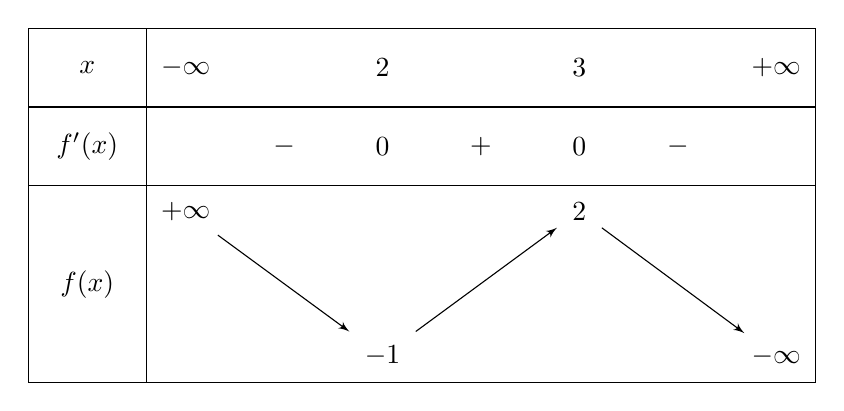
\begin{tikzpicture}
    \tkzTabInit[lgt=1.5, espcl=2.5]
    {$x$ /1, $f'(x)$ /1, $f(x)$ /2.5}
    {$-\infty$, $2$, $3$, $+\infty$}
    \tkzTabLine{, -, 0, +, 0, -, }
    \tkzTabVar{+/ $+\infty$ / , -/ $-1$ / , +/ $2$ / , -/ $-\infty$ /}
\end{tikzpicture}
\end{center}

Điểm cực đại của hàm số \( y = f(x) \) là}{
    \begin{tasks}(4)
        \task \( y = 2 \)
        \task \( x = 2 \)
        \task \( x = 3 \)
        \task \( y = -1 \)
    \end{tasks}
}

% --- CÂU 8 ---
\questionLinesManual{0}{8}{Hàm số nào sau đây có đồ thị là đường cong như hình vẽ?

\begin{center}
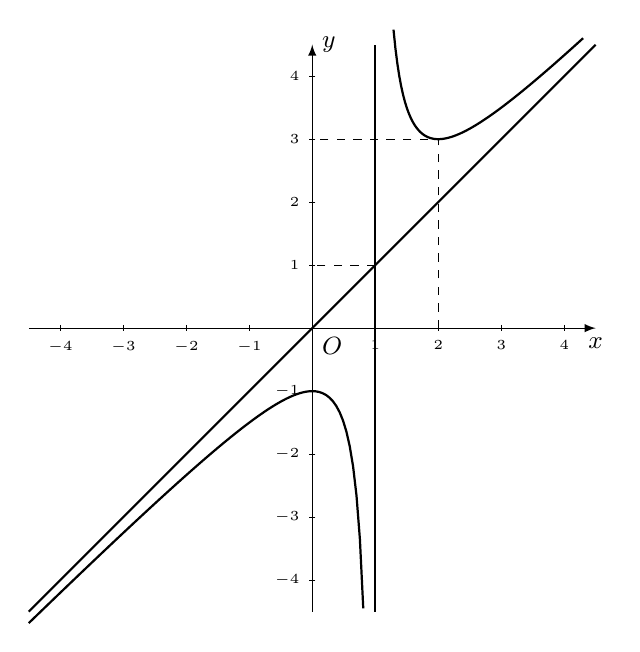
\begin{tikzpicture}[>=latex, scale=0.8]
    % 1. Hệ trục tọa độ
    \draw[->] (-4.5,0) -- (4.5,0) node[below] {\small $x$};
    \draw[->] (0,-4.5) -- (0,4.5) node[right] {\small $y$};
    \node[below right] at (0,0) {\small $O$};
    
    % 2. Đánh dấu các mốc
    \foreach \x in {-4,-3,-2,-1,1,2,3,4} {
        \draw (\x,0.05) -- (\x,-0.05) node[below] {\tiny $\x$};
    }
    \foreach \val in {-4,-3,-2,-1,1,2,3,4} {
        \draw (0.05,\val) -- (-0.05,\val) node[left] {\tiny $\val$};
    }
    
    % 3. Vẽ đồ thị hàm số y = (x^2 + x - 1)/(x - 1)
    \draw[thick, samples=100, domain=-4.5:0.81] 
        plot (\x, {(\x*\x - \x + 1)/(\x - 1)});
    \draw[thick, samples=100, domain=1.29:4.3] 
        plot (\x, {(\x*\x - \x +1)/(\x - 1)});
    \draw[thick, samples=100, domain=-4.5:4.5] 
        plot (\x, {(\x});
    % 4. Đường tiệm cận
    \draw[thick] (1,-4.5) -- (1,4.5) ;
    \draw[dashed] (1,1) -- (0,1);
    \draw[dashed] (2,0) -- ( 2,3) -- (0,3);
    
\end{tikzpicture}
\end{center}

}{
    \begin{tasks}(4)
        \task \( y = x - \dfrac{1}{x-1} \)
        \task \( y = -x + \dfrac{1}{x-1} \)
        \task \( y = -x - \dfrac{1}{x-1} \)
        \task \( y = x + \dfrac{1}{x-1} \)
    \end{tasks}
}

% --- CÂU 9 ---
\questionLinesManual{0}{9}{Đồ thị của hàm số nào dưới đây có dạng như đường cong trong hình vẽ?

\begin{center}
\begin{tikzpicture}[>=latex, scale=0.8]
                % 1. Hệ trục tọa độ
                \draw[->] (-3.5,0) -- (4.5,0) node[below] {\small $x$};
                \draw[->] (0,-3.5) -- (0,4.5) node[right] {\small $y$};
                \node[below left] at (0,0) {\small $O$};
                
                % 2. Đánh dấu các mốc
                \foreach \x in {-1,1,2} {
                    \draw (\x,0.05) -- (\x,-0.05) node[below] {\small $\x$};
                }
                \foreach \val in {-1,1,3} {
                    \draw (0.05,\val) -- (-0.05,\val) node[left] {\small $\val$};
                }
                
                % 3. Vẽ đồ thị hàm số y = (x+1)/(-x+1) = -(x+1)/(x-1)
                \draw[thick, samples=100, domain=-3.5:0.56] 
                    plot (\x, {(\x + 1)/(\x - 1)});
                \draw[thick, samples=100, domain=1.57:4.5] 
                    plot (\x, {(\x + 1)/(\x - 1)});
                
                % 4. Đường tiệm cận
                \draw[dashed] (1,-3.5) -- (1,4.5) ;
                \draw[dashed] (-3.5,1) -- (4.5,1);
                \draw[dashed] ( 2,0) -- ( 2,3) -- ( 0,3);
            \end{tikzpicture}
\end{center}

}{
    \begin{tasks}(4)
        \task \( y = \dfrac{2x - 1}{2x + 1} \)
        \task \( y = \dfrac{x + 1}{x - 1} \)
        \task \( y = \dfrac{2x + 1}{2x - 1} \)
        \task \( y = \dfrac{2x + 1}{x - 1} \)
    \end{tasks}
}

% --- CÂU 10 ---
\questionLinesManual{0}{10}{Cho hàm số \( y = f(x) \) liên tục trên \( \mathbb{R} \) và có đồ thị là đường cong trong hình dưới đây. Hàm số đã cho đồng biến trên khoảng nào dưới đây?

\begin{center}
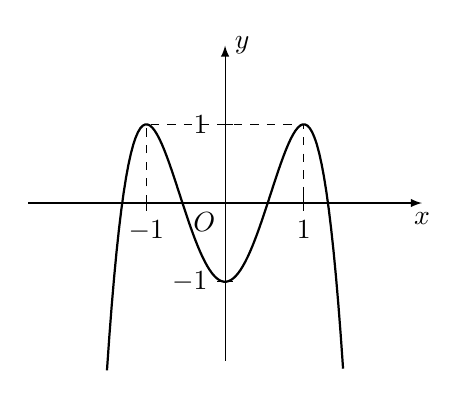
\begin{tikzpicture}[>=latex, scale=01]
    % Vẽ hệ trục
    \draw[->] (-2.5,0) -- (2.5,0) node[below] {$x$};
    \draw[->] (0,-2) -- (0,2) node[right] {$y$};
    \node[below left] at (0,0) {$O$};
    
    % Đánh dấu các mốc
    \draw (-1,0.1) -- (-1,-0.1) node[below] {$-1$};
    \draw (1,0.1) -- (1,-0.1) node[below] {$1$};
    \draw (0.1,1) -- (-0.1,1) node[left] {$1$};
    \draw (0.1,-1) -- (-0.1,-1) node[left] {$-1$};
    % Vẽ đồ thị hàm bậc 3
    \draw[thick, samples=100, domain=-1.5:1.5] 
        plot (\x, {-2*\x*\x*\x*\x + 4*\x*\x - 1});
    \draw[dashed] (-1,0) -- (-1,1) -- (1,1) -- (1,0);
\end{tikzpicture}
\end{center}

}{
    \begin{tasks}(4)
        \task $(0;1)$
        \task $(-1;1)$
        \task $(-\infty;1)$
        \task $(0;+\infty)$
    \end{tasks}
}

% --- CÂU 11 ---
\questionLinesManual{0}{11}{Số điểm cực tiểu của đồ thị hàm số \( y = \dfrac{1}{5}x^5 - \dfrac{3}{4}x^4 + \dfrac{2}{3}x^3 + \dfrac{1}{2} \) là}{
    \begin{tasks}(4)
        \task $0$
        \task $3$
        \task $2$
        \task $1$
    \end{tasks}
}

% --- CÂU 12 ---
\questionLinesManual{0}{12}{Cho hàm số \( f(x) \) xác định trên \( \mathbb{R} \) thỏa mãn đồng thời hai điều kiện: \( f(x) \) là hàm số lẻ và \( f(x) = x^2 \) với mọi \( x \leq 0 \). Giá trị của \( f(2) \) bằng}{
    \begin{tasks}(4)
        \task $-4$
        \task $-2$
        \task $0$
        \task $4$
    \end{tasks}
}

% --- CÂU 13 ---
\questionLinesManual{0}{13}{Giá trị cực tiểu của hàm số \( y = 4x^3 - 6x^2 + 11 \) bằng}{
    \begin{tasks}(4)
        \task $0$
        \task $1$
        \task $9$
        \task $11$
    \end{tasks}
}

% --- CÂU 14 ---
\questionLinesManual{0}{14}{Hàm số \( y = -2x^3 + 9x^2 + 24x - 114 \) đồng biến trên khoảng nào dưới đây?}{
    \begin{tasks}(4)
        \task $(-1; 4)$
        \task $(-4; -1)$
        \task $(-\infty; -1)$
        \task $(4; +\infty)$
    \end{tasks}
}

% --- CÂU 15 ---
\questionLinesManual{0}{15}{Cho hàm số \( f(x) \) liên tục trên \([-1; 5]\) và có đồ thị như hình vẽ bên (các điểm cực trị của đồ thị thể hiện rõ trên hình). Gọi \( M \) và \( m \) lần lượt là giá trị lớn nhất và nhỏ nhất của hàm số đã cho trên \([-1; 5]\). Giá trị của \( M - m \) bằng

\begin{center}
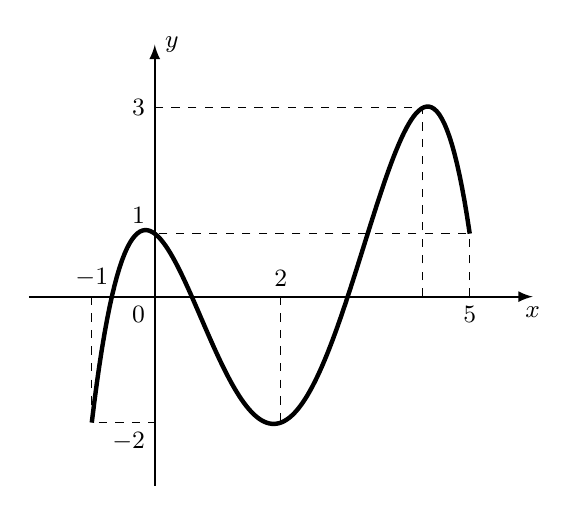
\begin{tikzpicture}[>=latex, scale=0.8]
    % 1. Hệ trục tọa độ Ox, Oy màu đen
    \draw[->, black, thick] (-2,0) -- (6,0) node[below] {\small $x$};
    \draw[->, black, thick] (0,-3) -- (0,4) node[right] {\small $y$};
    \node[below left] at (0,0) {\small $0$};
    
    % 2. Đồ thị hàm số màu đen
    \draw[black, ultra thick, samples=150, domain=-1:5] 
plot (\x, {-0.1588135590717*\x*\x*\x*\x + 1.2862146877635*\x*\x*\x - 2.3097740105484*\x*\x - 0.7548022573836*\x + 1});
    % 3. Các đường nét đứt và nhãn tọa độ màu đen
    % Tại x = -1, y = -2
    \draw[dashed, black] (-1,0) -- (-1,-2) -- (0,-2);
    \node[above] at (-1,0) {\small $-1$};
    \node[below left] at (0,-2) {\small $-2$};
    
    % Tại x = 0, y = 1
    \node[above left] at (0,1) {\small $1$};
    
    % Tại x = 2, y = -2
    \draw[dashed, black] (2,0) -- (2,-2);
    \node[above] at (2,0) {\small $2$};
    
    % Tại đỉnh cực đại thứ hai (x ≈ 4.25, y = 3)
    \draw[dashed, black] (4.25,0) -- (4.25,3) -- (0,3);
    \node[left] at (0,3) {\small $3$};
    
    % Tại điểm cuối cùng x = 5, y = 1
    \draw[dashed, black] (5,0) -- (5,1) -- (0,1);
    \node[below] at (5,0) {\small $5$};

\end{tikzpicture}
\end{center}

}{
    \begin{tasks}(4)
        \task $1$
        \task $4$
        \task $5$
        \task $6$
    \end{tasks}
}

% --- CÂU 16 ---
\questionLinesManual{0}{16}{Tiệm cận ngang của đồ thị hàm số \( y = \dfrac{2x - 4}{x + 2} \) là đường thẳng có phương trình}{
    \begin{tasks}(4)
        \task \( y = 2 \)
        \task \( y = -2 \)
        \task \( x = 2 \)
        \task \( x = -2 \)
    \end{tasks}
}

% --- CÂU 17 ---
\questionLinesManual{0}{17}{Đường tiệm cận ngang của đồ thị hàm số \( y = \dfrac{3x - 1}{1 - x} \) có phương trình là}{
    \begin{tasks}(4)
        \task \( x = -3 \)
        \task \( y = -3 \)
        \task \( x = 3 \)
        \task \( y = 3 \)
    \end{tasks}
}

% --- CÂU 18 ---
\questionLinesManual{0}{18}{Cho hàm số \( y = f(x) \) liên tục và có đồ thị trên đoạn \([-4;3]\) như hình vẽ. Giá trị nhỏ nhất của hàm số \( y = f(x) \) trên đoạn \([0;3]\) là

\begin{center}
\begin{tikzpicture}[>=latex, scale=0.8]
    % Vẽ hệ trục
    \draw[->] (-4.5,0) -- (4.5,0) node[below] {$x$};
    \draw[->] (0,-3.5) -- (0,3) node[right] {$y$};
    \node[below left] at (0,0) {$O$};
    
    % Đánh dấu các mốc
    \foreach \x in {-4,1,3} {
        \draw (\x,0.1) -- (\x,-0.1) node[below] {$\x$};
    }
    \foreach \y in {-3,-2,-1,2} {
        \draw (0.1,\y) -- (-0.1,\y) node[left] {$\y$};
    }
    
    % Vẽ đồ thị hàm số
    \draw[thick, samples=100, domain=0:3] 
       plot (\x, {\x*\x - 2*\x -1});
    \draw[thick] (-4,-3) -- (0,-1);
    \draw[dashed] (-4,0) -- (-4,-3) -- (0,-3);
    \draw[dashed] (1,0) -- (1,-2) -- (0,-2);
    \draw[dashed] (3,0) -- (3,2)-- (0,2);
    
\end{tikzpicture}
\end{center}

}{
    \begin{tasks}(4)
        \task $-4$
        \task $-3$
        \task $1$
        \task $-2$
    \end{tasks}
}

% --- CÂU 19 ---
\questionLinesManual{0}{19}{Cho hàm số \( y = f(x) \) liên tục trên \( \mathbb{R} \) và có bảng xét dấu đạo hàm như hình vẽ sau

\begin{center}
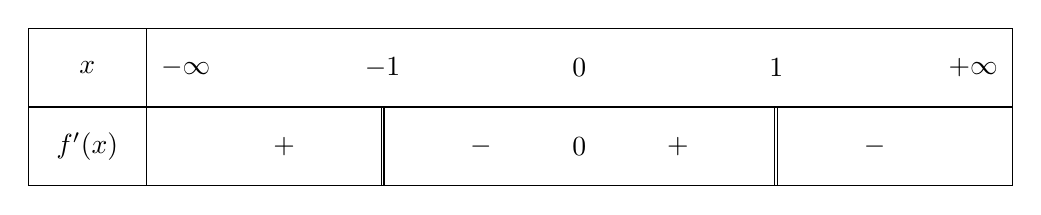
\begin{tikzpicture}
    \tkzTabInit[lgt=1.5, espcl=2.5]
    {$x$ /1, $f'(x)$ /1}
    {$-\infty$, $-1$ ,$0$, $1$, $+\infty$}
    \tkzTabLine{, +,d,-, 0, +, d, -, }
   
\end{tikzpicture}
\end{center}

Số điểm cực tiểu của đồ thị hàm số \( y = f(x) \) là}{
    \begin{tasks}(4)
        \task $2$
        \task $0$
        \task $1$
        \task $3$
    \end{tasks}
}

% --- CÂU 20 ---
\questionLinesManual{0}{20}{Cho hàm số bậc ba \( y = ax^3 + bx^2 + cx + d \) (\( a \neq 0 \)) có đồ thị như hình vẽ. Hàm số nghịch biến trên khoảng nào trong các khoảng dưới đây?

\begin{center}
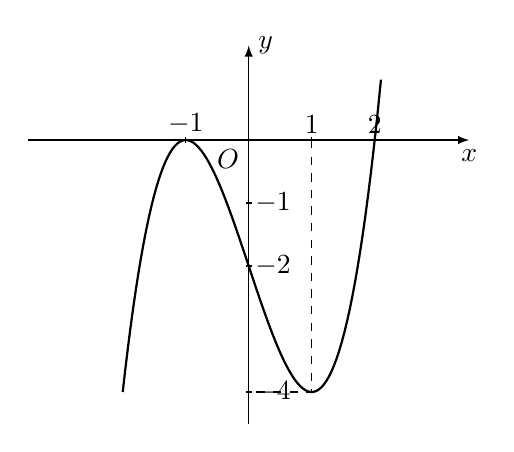
\begin{tikzpicture}[>=latex, scale=0.8]
    % Vẽ hệ trục
    \draw[->] (-3.5,0) -- (3.5,0) node[below] {$x$};
    \draw[->] (0,-4.5) -- (0,1.5) node[right] {$y$};
    \node[below left] at (0,0) {$O$};
    
    % Đánh dấu các mốc
    \foreach \x in {-1,1,2} {
        \draw (\x,0.05) -- (\x,-0.05) node[above] {$\x$};
    }
    \foreach \y in {-4,-2,-1} {
        \draw (0.05,\y) -- (-0.05,\y) node[right] {$\y$};
    }
    
    % Vẽ đồ thị hàm bậc 3
    \draw[thick, samples=100, domain=-2:2.1] 
        plot (\x, {\x^3 - 3*\x-2});
    \draw[dashed] (1,0) -- (1,-4) -- (0,-4);
    
\end{tikzpicture}
\end{center}

}{
    \begin{tasks}(4)
        \task $(-\infty; -1)$
        \task $(-1; 1)$
        \task $(1; +\infty)$
        \task $(-4; 0)$
    \end{tasks}
}

% --- CÂU 21 ---
\questionLinesManual{0}{21}{Điểm cực tiểu của hàm số \( y = \dfrac{1}{3}x^3 - 2x^2 + 3x - 1 \) là}{
    \begin{tasks}(4)
        \task \( x = \dfrac{1}{3} \)
        \task \( x = 3 \)
        \task \( x = -1 \)
        \task \( x = 1 \)
    \end{tasks}
}

% --- CÂU 22 ---
\questionLinesManual{0}{22}{Đường thẳng nào dưới đây là đường tiệm cận xiên của đồ thị hàm số \( y = 2x - 5 + \dfrac{10}{x + 3} \)?}{
    \begin{tasks}(4)
        \task \( y = 2x - 5 \)
        \task \( y = x + 3 \)
        \task \( y = 2x \)
        \task \( y = 2x + 3 \)
    \end{tasks}
}

% --- CÂU 23 ---
\questionLinesManual{0}{23}{Cho hàm số \( y = \dfrac{3x + 7}{x + 1} \). Giá trị lớn nhất của hàm số đã cho trên đoạn \([0; 3]\) bằng}{
    \begin{tasks}(4)
        \task $3$
        \task $7$
        \task $4$
        \task $0$
    \end{tasks}
}

% --- CÂU 24 ---
\questionLinesManual{0}{24}{Đường cong trong hình vẽ bên là đồ thị hàm số nào trong các hàm số được cho bởi các phương án dưới đây?
\begin{center}
\begin{tikzpicture}[>=latex, scale=0.8]
                % 1. Hệ trục tọa độ
                \draw[->] (-3.5,0) -- (4.5,0) node[below] {\small $x$};
                \draw[->] (0,-3.5) -- (0,4.5) node[right] {\small $y$};
                \node[below left] at (0,0) {\small $O$};
                
                % 2. Đánh dấu các mốc
                \foreach \x in {-1,1} {
                    \draw (\x,0.05) -- (\x,-0.05) node[below] {\small $\x$};
                }
                \foreach \val in {-1,1} {
                    \draw (0.05,\val) -- (-0.05,\val) node[left] {\small $\val$};
                }
                
                % 3. Vẽ đồ thị hàm số y = (x+1)/(-x+1) = -(x+1)/(x-1)
                \draw[thick, samples=100, domain=-3.5:0.56] 
                    plot (\x, {(\x + 1)/(\x - 1)});
                \draw[thick, samples=100, domain=1.57:4.5] 
                    plot (\x, {(\x + 1)/(\x - 1)});
                
                % 4. Đường tiệm cận
                \draw[dashed] (1,-3.5) -- (1,4.5) ;
                \draw[dashed] (-3.5,1) -- (4.5,1);
               
            \end{tikzpicture}
\end{center}}
{
    \begin{tasks}(4)
        \task \( y = \dfrac{2x - 1}{x - 1} \)
        \task \( y = \dfrac{x + 1}{x - 1} \)
        \task \( y = \dfrac{2x - 2}{2x + 1} \)
        \task \( y = \dfrac{-x + 1}{x + 1} \)
    \end{tasks}
}

% --- CÂU 25 ---
\questionLinesManual{0}{25}{Cho hàm số \( y = f(x) \) xác định trên \( \mathbb{R} \), có bảng biến thiên như hình vẽ dưới đây. Hàm số \( y = f(x) \) nghịch biến trên khoảng nào trong các khoảng sau?

\begin{center}
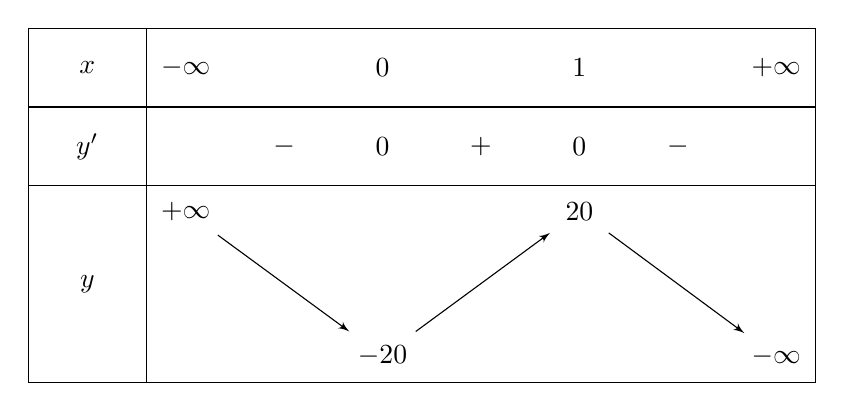
\begin{tikzpicture}
    \tkzTabInit[lgt=1.5, espcl=2.5]
    {$x$ /1, $y'$ /1, $y$ /2.5}
    {$-\infty$, $0$, $1$, $+\infty$}
    \tkzTabLine{, -, 0, +, 0, -, }
    \tkzTabVar{+/ $+\infty$ / , -/ $-20$ / , +/ $20$ / , -/ $-\infty$ /}
\end{tikzpicture}
\end{center}

}{
    \begin{tasks}(4)
        \task $(0;1)$
        \task $(-\infty;22)$
        \task $(0;+\infty)$
        \task $(2;+\infty)$
    \end{tasks}
}


% --- CÂU 26 ---
\questionLinesManual{0}{26}{Hàm số \( f(x) \) có đạo hàm \( f'(x) = x^2(x-1)(x-2)^3 \), \( \forall x \in \mathbb{R} \). Hàm số \( f(x) \) có bao nhiêu điểm cực đại?}{
    \begin{tasks}(4)
        \task $2$
        \task $0$
        \task $1$
        \task $3$
    \end{tasks}
}

% --- CÂU 27 ---
\questionLinesManual{0}{27}{Đồ thị có hình vẽ dưới đây là của hàm số nào?

\begin{center}
\begin{tikzpicture}[>=latex, scale=0.8]
                % 1. Hệ trục tọa độ
                \draw[->] (-4.5,0) -- (3.5,0) node[below] {\small $x$};
                \draw[->] (0,-4.5) -- (0,3.5) node[right] {\small $y$};
                \node[below left] at (0,0) {\small $O$};
                
                % 2. Đánh dấu các mốc
                \foreach \x in {-3,-1,1} {
                    \draw (\x,0.05) -- (\x,-0.05) node[below] {\small $\x$};
                }
                \foreach \val in {-2,-1,1} {
                    \draw (0.05,\val) -- (-0.05,\val) node[below left] {\small $\val$};
                }
                
                % 3. Vẽ đồ thị hàm số y = (x+1)/(-x+1) = -(x+1)/(x-1)
                \draw[thick, samples=100, domain=-4.5:-1.57] 
                    plot (\x, {(\x - 1)/(-\x - 1)});
                \draw[thick, samples=100, domain=-0.56:3.5] 
                    plot (\x, {(\x - 1)/(-\x - 1)});
                
                % 4. Đường tiệm cận
                \draw[dashed] (-1,-4.5) -- (-1,3.5);
                \draw[dashed] (-4.5,-1) -- (3.5,-1);
                \draw[dashed] ( -3,0) -- ( -3,-2) -- (0,-2);
            \end{tikzpicture}
\end{center}

}{
    \begin{tasks}(4)
        \task \( y = \dfrac{-x + 2}{x + 1} \)
        \task \( y = \dfrac{-x}{x + 1} \)
        \task \( y = \dfrac{-x + 1}{x + 1} \)
        \task \( y = \dfrac{-2x + 1}{2x + 1} \)
    \end{tasks}
}

% --- CÂU 28 ---
\questionLinesManual{0}{28}{Cho hàm số \( y = f(x) \) có đồ thị như hình bên. Hàm số đã cho đạt giá trị nhỏ nhất trên đoạn \([-1; 1]\) tại

\begin{center}
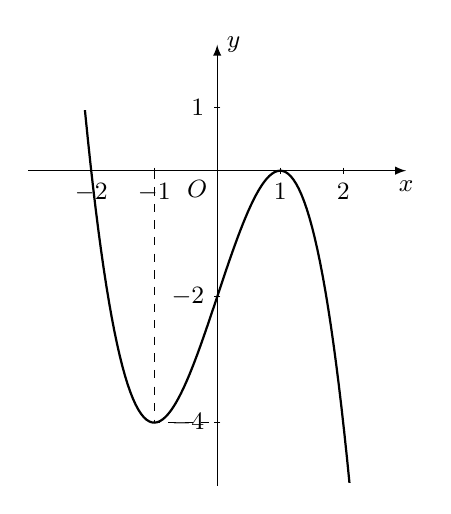
\begin{tikzpicture}[>=latex, scale=0.8]
    % Hệ trục tọa độ
    \draw[->] (-3,0) -- (3,0) node[below] {\small $x$};
    \draw[->] (0,-5) -- (0,2) node[right] {\small $y$};
    \node[below left] at (0,0) {\small $O$};
    
    % Đánh dấu các mốc
    \foreach \x in {-2,-1,1,2} {
         \draw (\x,0.05) -- (\x,-0.05)  node[below] {\small $\x$};
    }
    \foreach \y in {-4,-2,1} {
          \draw (0.05,\y) -- (-0.05,\y)   node[left] {\small $\y$};
    }
    
    % Đồ thị hàm bậc 3: y = x^3 - 3x + 1
    \draw[thick, samples=100, domain=-2.1:2.1] 
        plot (\x, {-\x*\x*\x + 3*\x-2});
    
    \draw[dashed] (-1,0) -- (-1,-4) -- (0,-4);
    
\end{tikzpicture}
\end{center}

}{
    \begin{tasks}(4)
        \task $x = -1$
        \task $x = 0$
        \task $x = -4$
        \task $x = 1$
    \end{tasks}
}

% --- CÂU 29 ---
\questionLinesManual{0}{29}{Cho hàm số \( y = f(x) \) có bảng biến thiên như hình bên dưới.

\begin{center}
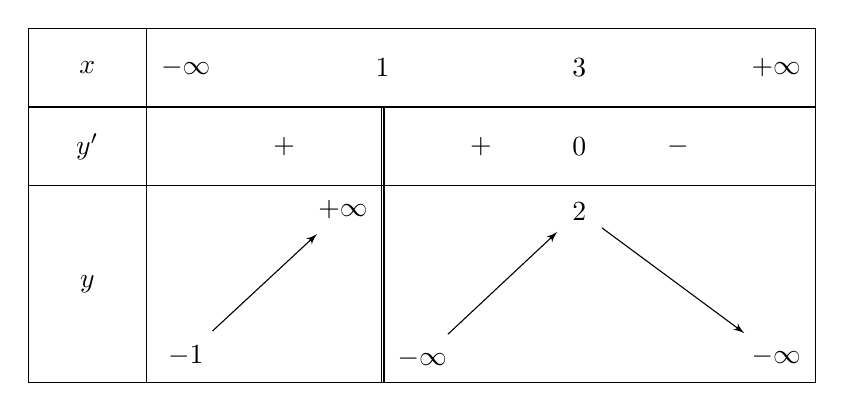
\begin{tikzpicture}
    \tkzTabInit[lgt=1.5, espcl=2.5]
    {$x$ /1, $y'$ /1, $y$ /2.5}
    {$-\infty$, $1$, $3$, $+\infty$}
    \tkzTabLine{, +, d, +, 0, -, }
    \tkzTabVar{-/ $-1$ / , +D- /$+\infty$ /$-\infty$, +/ $2$ / , -/ $-\infty$ /}
\end{tikzpicture}
\end{center}

Đồ thị hàm số \( y = f(x) \) có tổng số bao nhiêu đường tiệm cận đứng và ngang?}{
    \begin{tasks}(4)
        \task $2$
        \task $0$
        \task $1$
        \task $3$
    \end{tasks}
}

% --- CÂU 30 ---
\questionLinesManual{0}{30}{Cho hàm số \( y = f(x) \) có bảng biến thiên như sau:

\begin{center}
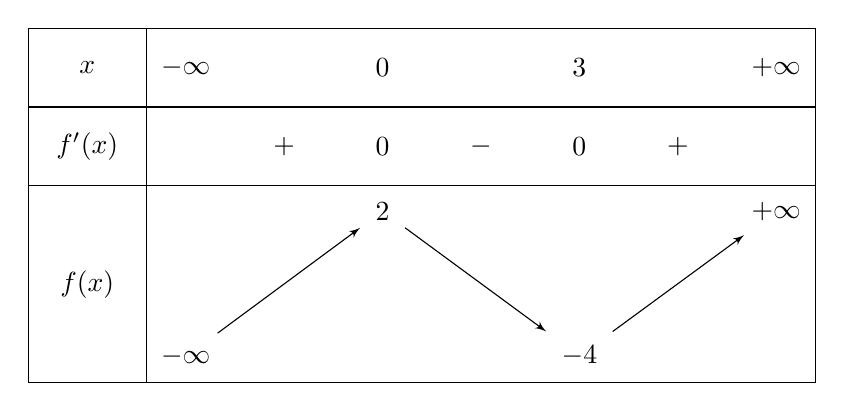
\begin{tikzpicture}
    \tkzTabInit[lgt=1.5, espcl=2.5]
    {$x$ /1, $f'(x)$ /1, $f(x)$ /2.5}
    {$-\infty$, $0$, $3$, $+\infty$}
    \tkzTabLine{, +, 0, -, 0, +, }
    \tkzTabVar{-/ $-\infty$ / , +/ $2$ / , -/ $-4$ / , +/ $+\infty$ /}
\end{tikzpicture}
\end{center}

Hàm số \( f(x) \) đạt cực tiểu tại điểm}{
    \begin{tasks}(4)
        \task \( y = 0 \)
        \task \( x = -4 \)
        \task \( y = -4 \)
        \task \( x = 3 \)
    \end{tasks}
}

% --- CÂU 31 ---
\questionLinesManual{0}{31}{Cho hàm số \( f(x) \) có bảng xét dấu của đạo hàm như sau:

\begin{center}
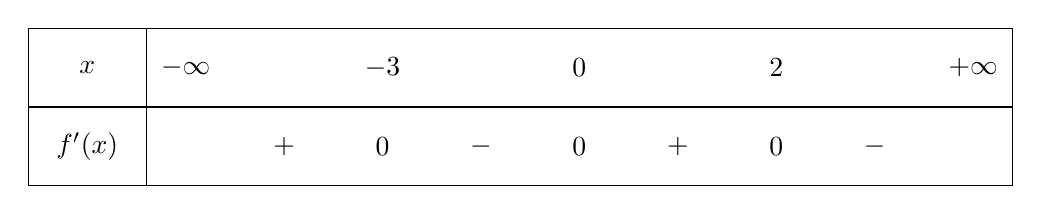
\begin{tikzpicture}
    \tkzTabInit[lgt=1.5, espcl=2.5]
    {$x$ /1, $f'(x)$ /1}
    {$-\infty$,$-3$, $0$, $2$, $+\infty$}
    \tkzTabLine{, +, 0, -, 0, +,0,- }
    
\end{tikzpicture}
\end{center}

Hàm số đã cho nghịch biến trên khoảng nào dưới đây?}{
    \begin{tasks}(4)
        \task $(-3; 0)$
        \task $(0; +\infty)$
        \task $(0; 2)$
        \task $(-\infty; -3)$
    \end{tasks}
}

% --- CÂU 32 ---
\questionLinesManual{0}{32}{Bảng biến thiên sau đây là của hàm số nào?

\begin{center}
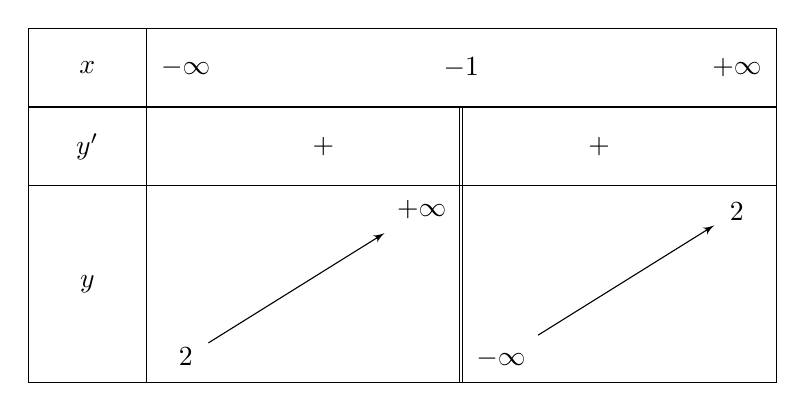
\begin{tikzpicture}
    \tkzTabInit[lgt=1.5, espcl=3.5]
    {$x$ /1, $y'$ /1, $y$ /2.5}
    {$-\infty$, $-1$, $+\infty$}
    \tkzTabLine{, +, d, +, }
    \tkzTabVar{-/ $2$ / , +D-/ $+\infty$ / $-\infty$, +/ $2$ /}
\end{tikzpicture}
\end{center}

}{
    \begin{tasks}(4)
        \task \( y = \dfrac{2x+3}{x+1} \)
        \task \( y = \dfrac{2x-1}{x-1} \)
        \task \( y = \dfrac{2x-1}{x+1} \)
        \task \( y = \dfrac{x+1}{2x-1} \)
    \end{tasks}
}

% --- CÂU 33 ---
\questionLinesManual{0}{33}{Đường cong trong hình sau là của hàm số nào dưới đây?

\begin{center}
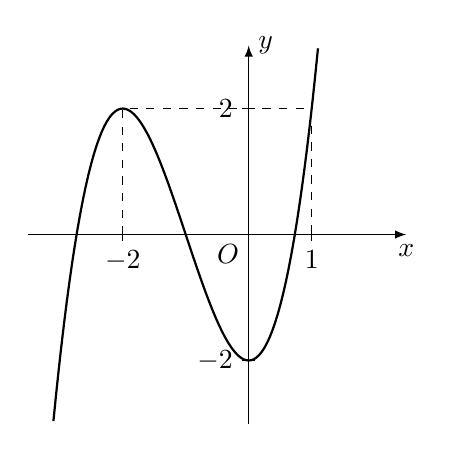
\begin{tikzpicture}[>=latex, scale=0.8]
    % Vẽ hệ trục
    \draw[->] (-3.5,0) -- (2.5,0) node[below] {$x$};
    \draw[->] (0,-3) -- (0,3) node[right] {$y$};
    \node[below left] at (0,0) {$O$};
    
    % Đánh dấu các mốc
    \foreach \x in {-2,1} {
        \draw (\x,0.1) -- (\x,-0.1) node[below] {$\x$};
    }
    \foreach \y in {-2,2} {
        \draw (0.1,\y) -- (-0.1,\y) node[left] {$\y$};
    }
    
    % Vẽ đồ thị hàm số y = x^3 + 3x^2 - 2
    \draw[thick, samples=100, domain=-3.1:1.1] 
       plot (\x, {\x*\x*\x + 3*\x*\x - 2});
    \draw[dashed] (-2,0) -- (-2,2) -- (1,2) --(1,0);
\end{tikzpicture}
\end{center}

}{
    \begin{tasks}(4)
        \task \( y = -x^3 - 3x^2 - 2 \)
        \task \( y = x^3 - 3x^2 - 2 \)
        \task \( y = 2x^3 + 6x^2 - 2 \)
        \task \( y = x^3 + 3x^2 - 2 \)
    \end{tasks}
}

% --- CÂU 34 ---
\questionLinesManual{0}{34}{Tìm giá trị lớn nhất của hàm số \( y = \dfrac{2x + 3}{x - 1} \) trên đoạn \([2; 4]\).}{
    \begin{tasks}(4)
        \task $8$
        \task $\dfrac{9}{2}$
        \task $7$
        \task $\dfrac{11}{3}$
    \end{tasks}
}

% --- CÂU 35 ---
\questionLinesManual{0}{35}{Giá trị lớn nhất của hàm số \( y = 3\sin 2x - 1 \) là}{
    \begin{tasks}(4)
        \task $2$
        \task $5$
        \task $4$
        \task $3$
    \end{tasks}
}

% --- CÂU 36 ---
\questionLinesManual{0}{36}{Cho hàm số \( f(x) = ax^3 + bx^2 + cx + d \) có đồ thị như hình sau đây.

\begin{center}
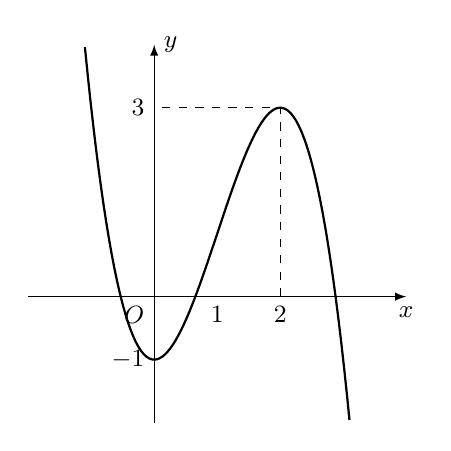
\begin{tikzpicture}[>=latex, scale=0.8]
    % Hệ trục tọa độ
    \draw[->] (-2,0) -- (4,0) node[below] {\small $x$};
    \draw[->] (0,-2) -- (0,4) node[right] {\small $y$};
    \node[below left] at (0,0) {\small $O$};
    
    
    % Đồ thị hàm bậc 3: y = x^3 - 3x
    \draw[thick, samples=100, domain=-1.1:3.1] 
        plot (\x, {-\x*\x*\x + 3*\x*\x - 1});
    
    % Đánh dấu điểm cực trị
    \draw[dashed] (2,0) -- (2,3) -- (0,3);
    \node[below] at (1,0) {\small $1$};
    \node[below] at (2,0) {\small $2$};
    \node[left] at (0,3) {\small $3$};
    \node[left] at (0,-1) {\small $-1$};
\end{tikzpicture}
\end{center}

Số nghiệm dương của phương trình \( 2f(x) - 3 = 0 \) là:}{
    \begin{tasks}(4)
        \task $1$
        \task $0$
        \task $3$
        \task $2$
    \end{tasks}
}

% --- CÂU 37 ---
\questionLinesManual{0}{37}{Cho hàm số \( y = f(x) \) có bảng biến thiên như sau

\begin{center}
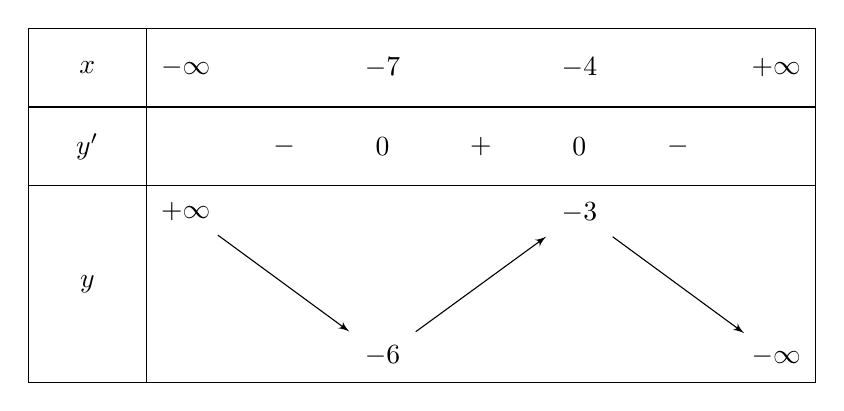
\begin{tikzpicture}
    \tkzTabInit[lgt=1.5, espcl=2.5]
    {$x$ /1, $y'$ /1, $y$ /2.5}
    {$-\infty$, $-7$, $-4$, $+\infty$}
    \tkzTabLine{, -, 0, +, 0, -, }
    \tkzTabVar{+/ $+\infty$ / , -/ $-6$ / , +/ $-3$ / , -/ $-\infty$ /}
\end{tikzpicture}
\end{center}

Giá trị cực đại của hàm số \( y = f(x) \) là}{
    \begin{tasks}(4)
        \task \( y = -3 \)
        \task \( y = -6 \)
        \task \( x = -7 \)
        \task \( x = -4 \)
    \end{tasks}
}

% --- CÂU 38 ---
\questionLinesManual{0}{38}{Đường tiệm cận xiên của đồ thị hàm số \( y = x + 4 + \dfrac{x - 1}{x - 2} \) là}{
    \begin{tasks}(4)
        \task \( y = x + 4 \)
        \task \( x = 2 \)
        \task \( y = x + 5 \)
        \task \( y = x + 3 \)
    \end{tasks}
}

% --- CÂU 39 ---
\questionLinesManual{0}{39}{Cho hàm số \( y = \dfrac{ax + 2}{x + c} \) có đồ thị như hình sau đây. Tính giá trị của biểu thức \( P = 2a - c \).

\begin{center}
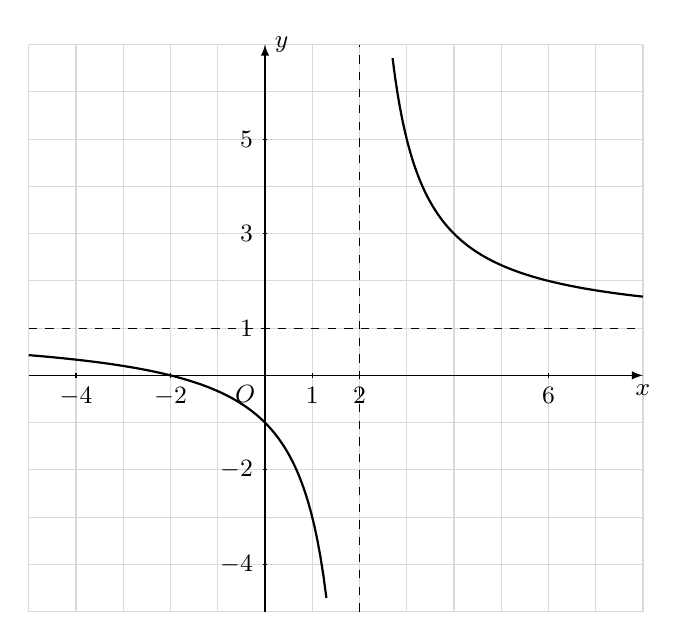
\begin{tikzpicture}[>=latex, scale=0.6]
    % 1. Vẽ lưới
    \draw[color=gray!30, thin, step=1] (-5,-5) grid (8,7);
    
    % 2. Vẽ hệ trục tọa độ
    \draw[->] (-5,0) -- (8,0) node[below] {\small $x$};
    \draw[->] (0,-5) -- (0,7) node[right] {\small $y$};
    \node[below left] at (0,0) {\small $O$};
    
    % 3. Đánh dấu các mốc
    \foreach \x in {-4,-2,1,2,6} {
        \draw (\x,0.05) -- (\x,-0.05) node[below] {\small $\x$};
    }
    \foreach \val in {-4,-2,1,3,5} {
        \draw (0.05,\val) -- (-0.05,\val) node[left] {\small $\val$};
    }
    
    % 4. Vẽ đồ thị hàm số y = (2x+1)/(x+1)
    \draw[thick, samples=100, domain=-5:1.3] 
        plot (\x, {(\x + 2)/(\x -2)});
    \draw[thick, samples=100, domain=2.7:8] 
        plot (\x, {(\x + 2)/(\x - 2)});
    
    % 5. Đường tiệm cận
    \draw[dashed] (2,-5) -- (2,7);
    \draw[dashed] (-5,1) -- (8,1);
\end{tikzpicture}
\end{center}

}{
    \begin{tasks}(4)
        \task $4$
        \task $-4$
        \task $-5$
        \task $5$
    \end{tasks}
}


% --- CÂU 40 ---
\questionLinesManual{0}{40}{Bạn Hải có một tấm bìa hình vuông cạnh 40 cm. Bạn muốn cắt bỏ ở bốn góc bốn hình vuông nhỏ bằng nhau để gấp và dán lại thành một hộp hình hộp chữ nhật không có nắp (tham khảo hình vẽ).
\begin{center}
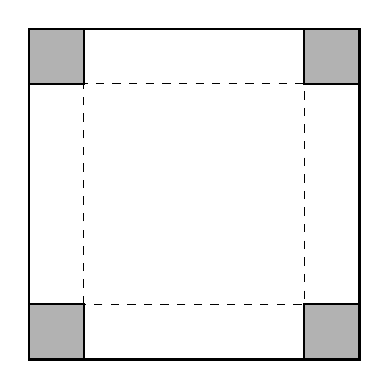
\begin{tikzpicture}[scale=0.35, >=stealth]
    % --- HÌNH 1: MẢNH CÁC TẤM BÌA PHẲNG ---
    % Khai báo kích thước tổng thể và cạnh cắt x
    \def\a{12}
    \def\x{2}
    
    % Tô màu xám cho 4 góc bị cắt
    \fill[gray!60] (0,0) rectangle (\x,\x);
    \fill[gray!60] (0,\a-\x) rectangle (\x,\a);
    \fill[gray!60] (\a-\x,0) rectangle (\a,\x);
    \fill[gray!60] (\a-\x,\a-\x) rectangle (\a,\a);
    \draw[thick] (0,0) rectangle (\x,\x);
    \draw[thick] (0,\a-\x) rectangle (\x,\a);
    \draw[thick] (\a-\x,0) rectangle (\a,\x);
    \draw[thick] (\a-\x,\a-\x) rectangle (\a,\a);
    % Vẽ biên ngoài hình vuông lớn
    \draw[thick] (0,0) rectangle (\a,\a);
    \draw[dashed] (\x,\x) rectangle (\a-\x,\a-\x);

    
    
\end{tikzpicture}
\quad \quad \quad
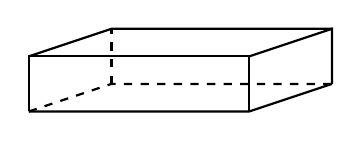
\begin{tikzpicture}[scale=0.35, >=stealth]
    % --- HÌNH 2: HÌNH HỘP CHỮ NHẬT 3D KHÔNG NẮP ---
    % Định nghĩa các điểm tọa độ mặt đáy
    \coordinate (A) at (0,0);
    \coordinate (B) at (8,0);
    \coordinate (C) at (11,1);
    \coordinate (D) at (3,1);
    
    % Chiều cao hộp h
    \def\h{2}
    
    % Các điểm mặt trên
    \coordinate (A1) at (0,\h);
    \coordinate (B1) at (8,\h);
    \coordinate (C1) at (11,3);
    \coordinate (D1) at (3,3);
    
    % Vẽ các nét khuất (nét đứt phía sau)
    \draw[dashed, thick] (A) -- (D) -- (C);
    \draw[dashed, thick] (D) -- (D1);
    
    % Vẽ các nét thấy phía trước và mặt trên mở
    \draw[thick] (A) -- (B) -- (C);
    \draw[thick] (A) -- (A1) -- (B1) -- (B);
    \draw[thick] (B1) -- (C1) -- (C);
    \draw[thick] (A1) -- (D1) -- (C1);
    
\end{tikzpicture}
\end{center}
Để hộp có thể tích lớn nhất thì độ dài cạnh của hình vuông nhỏ bị cắt là:}{
    \begin{tasks}(4)
        \task $6$ cm
        \task $5$ cm
        \task $\dfrac{20}{3}$ cm
        \task $\dfrac{10}{3}$ cm
    \end{tasks}
}

% --- CÂU 41 ---
\questionLinesManual{0}{41}{Hàm số nào sau đây nghịch biến trên \( \mathbb{R} \)?}{
    \begin{tasks}(4)
        \task \( y = \left( \dfrac{2026}{2025} \right)^x \)
        \task \( y = \log_1 x \)
        \task \( y = \dfrac{2x - 1}{x - 1} \)
        \task \( y = e^{-x} \)
    \end{tasks}
}

% --- CÂU 42 ---
\questionLinesManual{0}{42}{Cho hàm số \( f(x) = ax^3 + bx^2 + cx + d \) có đồ thị như hình sau đây.

\begin{center}
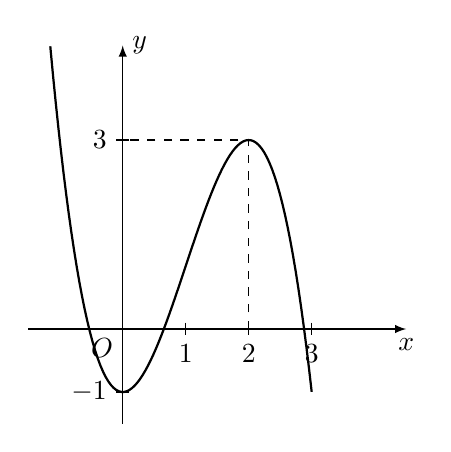
\begin{tikzpicture}[>=latex, scale=0.8]
    % Vẽ hệ trục
    \draw[->] (-1.5,0) -- (4.5,0) node[below] {$x$};
    \draw[->] (0,-1.5) -- (0,4.5) node[right] {$y$};
    \node[below left] at (0,0) {$O$};
    
    % Đánh dấu các mốc
    \foreach \x in {1,2,3} {
        \draw (\x,0.1) -- (\x,-0.1) node[below] {$\x$};
    }
    \foreach \y in {-1,3} {
        \draw (0.1,\y) -- (-0.1,\y) node[left] {$\y$};
    }
    
    % Vẽ đồ thị hàm bậc 3
    \draw[thick, samples=100, domain=-1.15:3] 
       plot (\x, {-\x*\x*\x + 3*\x*\x - 1});
    \draw[dashed] (2,0) -- (2,3) -- (0,3);
\end{tikzpicture}
\end{center}

Điểm cực đại của hàm số \( y = f(x) \) là}{
    \begin{tasks}(4)
        \task \( x = 0 \)
        \task \( x = 2 \)
        \task \( y = 3 \)
        \task \( M(2; 3) \)
    \end{tasks}
}

% --- CÂU 43 ---
\questionLinesManual{0}{43}{Đường tiệm cận đứng của đồ thị hàm số \( y = \dfrac{2x + 3}{x - 1} \) là}{
    \begin{tasks}(4)
        \task \( x = 2 \)
        \task \( y = 1 \)
        \task \( y = 2 \)
        \task \( x = 1 \)
    \end{tasks}
}

% --- CÂU 44 ---
\questionLinesManual{0}{44}{Cho hàm số \( y = f(x) \) có đạo hàm \( f'(x) = x^2(x+1)^2(2x-1) \). Số điểm cực trị của hàm số \( y = f(x) \) là}{
    \begin{tasks}(4)
        \task $3$
        \task $0$
        \task $2$
        \task $1$
    \end{tasks}
}

% --- CÂU 45 ---
\questionLinesManual{0}{45}{Giá trị nhỏ nhất của hàm số \( y = x^3 - 3x + 5 \) trên đoạn \([2; 4]\) là}{
    \begin{tasks}(4)
        \task \( \min_{[2;4]} y = 5 \)
        \task \( \min_{[2;4]} y = 0 \)
        \task \( \min_{[2;4]} y = 3 \)
        \task \( \min_{[2;4]} y = 7 \)
    \end{tasks}
}

% --- CÂU 46 ---
\questionLinesManual{0}{46}{Hàm số \( y = f(x) \) có đồ thị như hình dưới đây. Đồ thị hàm số đã cho có đường tiệm cận ngang là:

\begin{center}
\begin{tikzpicture}[>=latex, scale=0.6]
   
    
    % 2. Vẽ hệ trục tọa độ
    \draw[->] (-5,0) -- (8,0) node[below] {\small $x$};
    \draw[->] (0,-5) -- (0,7) node[right] {\small $y$};
    \node[below left] at (0,0) {\small $O$};
    
    % 3. Đánh dấu các mốc
    \foreach \x in {2} {
        \draw (\x,0.05) -- (\x,-0.05) node[below] {\small $\x$};
    }
    \foreach \val in {1} {
        \draw (0.05,\val) -- (-0.05,\val) node[left] {\small $\val$};
    }
    
    % 4. Vẽ đồ thị hàm số y = (2x+1)/(x+1)
    \draw[thick, samples=100, domain=-5:1.3] 
        plot (\x, {(\x + 2)/(\x -2)});
    \draw[thick, samples=100, domain=2.7:8] 
        plot (\x, {(\x + 2)/(\x - 2)});
    
    % 5. Đường tiệm cận
    \draw[dashed] (2,-5) -- (2,7);
    \draw[dashed] (-5,1) -- (8,1);
\end{tikzpicture}
\end{center}

}{
    \begin{tasks}(4)
        \task \( x = 2 \)
        \task \( x = 1 \)
        \task \( y = 1 \)
        \task \( y = 2 \)
    \end{tasks}
}

% --- CÂU 47 ---
\questionLinesManual{0}{47}{Hình vẽ sau đây là đồ thị của một trong bốn hàm số cho ở các đáp án. Hỏi đó là hàm số nào?

\begin{center}
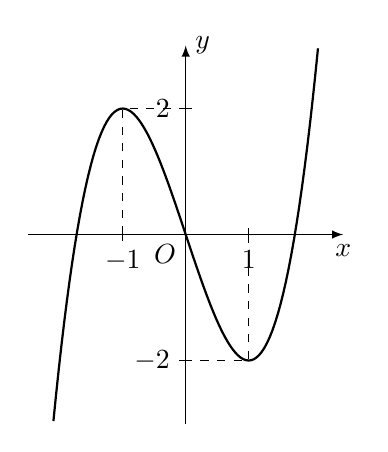
\begin{tikzpicture}[>=latex, scale=0.8]
    % Vẽ hệ trục
    \draw[->] (-2.5,0) -- (2.5,0) node[below] {$x$};
    \draw[->] (0,-3) -- (0,3) node[right] {$y$};
    \node[below left] at (0,0) {$O$};
    
    % Đánh dấu các mốc
    \foreach \x in {-1,1} {
        \draw (\x,0.1) -- (\x,-0.1) node[below] {$\x$};
    }
    \foreach \y in {-2,2} {
        \draw (0.1,\y) -- (-0.1,\y) node[left] {$\y$};
    }
    
    % Vẽ đồ thị hàm bậc 3
    \draw[thick, samples=100, domain=-2.1:2.1] 
        plot (\x, {\x^3 - 3*\x});
    \draw[dashed] (1,0) -- (1,-2) -- (0,-2);
    \draw[dashed] ( -1,0) -- (-1,2) -- (0,2);
\end{tikzpicture}
\end{center}

}{
    \begin{tasks}(4)
        \task \( y = x^3 + 2x + 1 \)
        \task \( y = x^3 - 3x \)
        \task \( y = -x^3 + 3x \)
        \task \( y = x^3 + 3x^2 \)
    \end{tasks}
}

% --- CÂU 48 ---
\questionLinesManual{0}{48}{Cho hàm số \( y = f(x) \) có đạo hàm \( f'(x) = (2x - 1)(x + 1) \). Hàm số \( y = f(x) \) có giá trị lớn nhất trên \([-2; 0]\) bằng}{
    \begin{tasks}(4)
        \task \( f\left(-\dfrac{1}{2}\right) \)
        \task \( f(-1) \)
        \task \( f(0) \)
        \task \( f(-2) \)
    \end{tasks}
}

% --- CÂU 49 ---
\questionLinesManual{0}{49}{Số đường tiệm cận của đồ thị hàm số \( y = 2x + 3 + \dfrac{1}{x - 1} \) là}{
    \begin{tasks}(4)
        \task $0$
        \task $3$
        \task $1$
        \task $2$
    \end{tasks}
}

% --- CÂU 50 ---
\questionLinesManual{0}{50}{Cho hàm số \( y = f(x) \) có đạo hàm trên \( \mathbb{R} \). Biết hàm số \( y = f'(x) \) có đồ thị như hình vẽ. Phát biểu nào sau đây là đúng?

\begin{center}
\begin{tikzpicture}[>=latex, scale=0.8]
    % Hệ trục tọa độ
    \draw[->] (-3.5,0) -- (3.5,0) node[below] {$x$};
    \draw[->] (0,-2) -- (0,3.5) node[right] {$y$};
    \node[above left] at (0,0) {$O$};
    
    % Đánh dấu các điểm
    \node[below] at (-2,0) {$-2$};
    \node[below] at (1,0) {$1$};
    \node[right] at (0,2) {$2$};
    
    % Vẽ đồ thị f'(x) là parabol hướng xuống có nghiệm tại x = -2 và x = 1
    \draw[thick, color=black!80, samples=150, domain=-2.3:1.3] 
        plot (\x, {-(\x+2)*(\x-1)});
    
    \node[right] at (1.5,2) {$y = f'(x)$};
\end{tikzpicture}
\end{center}}

{
    \begin{tasks}(1)
        \task Hàm số \( y = f(x) \) đạt cực đại tại \( x_1 = -2 \) và đạt cực tiểu tại \( x_2 = 1 \).
        \task Hàm số \( y = f(x) \) đạt cực tiểu tại hai điểm \( x_1 = -2 \) và \( x_2 = 1 \).
        \task Hàm số \( y = f(x) \) đạt cực đại tại hai điểm \( x_1 = -2 \) và \( x_2 = 1 \).
        \task Hàm số \( y = f(x) \) đạt cực tiểu tại \( x_1 = -2 \) và đạt cực đại tại \( x_2 = 1 \).
    \end{tasks}
}

% --- CÂU 51 ---
\questionLinesManual{0}{51}{Tiệm cận xiên của đồ thị hàm số \( y = \dfrac{x^2 + x + 2}{x + 2} \) là}{
    \begin{tasks}(4)
        \task \( y = x - 1 \)
        \task \( y = x + 1 \)
        \task \( y = x - 2 \)
        \task \( y = x + 2 \)
    \end{tasks}
}

% --- CÂU 52 ---
\questionLinesManual{0}{52}{Cho hàm số \( y = \dfrac{3x - 5}{x + 1} \). Tâm đối xứng của đồ thị hàm số là điểm nào?}{
    \begin{tasks}(4)
        \task \( M(-1;3) \)
        \task \( N(3;-1) \)
        \task \( P(-1;5) \)
        \task \( Q(-5;1) \)
    \end{tasks}
}

% --- CÂU 53 ---
\questionLinesManual{0}{53}{Bạn Long định gấp một cái hộp có dạng hình lăng trụ tứ giác đều với tổng diện tích tất cả các mặt là \( 96 \, cm^2 \). Thể tích cái hộp mà bạn Long định gấp lớn nhất bằng bao nhiêu?}{
    \begin{tasks}(4)
        \task \( 32 \, cm^3 \)
        \task \( 64 \, cm^3 \)
        \task \( 108 \, cm^3 \)
        \task \( 96 \, cm^3 \)
    \end{tasks}
}

% --- CÂU 54 ---
\questionLinesManual{0}{54}{Giá trị nhỏ nhất của hàm số \( y = x^4 - 2x^2 + 3 \) trên đoạn \([0;2]\) bằng}{
    \begin{tasks}(4)
        \task $2$
        \task $-2$
        \task $4$
        \task $3$
    \end{tasks}
}

% --- CÂU 55 ---
\questionLinesManual{0}{55}{Cho hàm số \( y = f(x) \) liên tục trên \( \mathbb{R} \) và có bảng biến thiên như sau:

\begin{center}
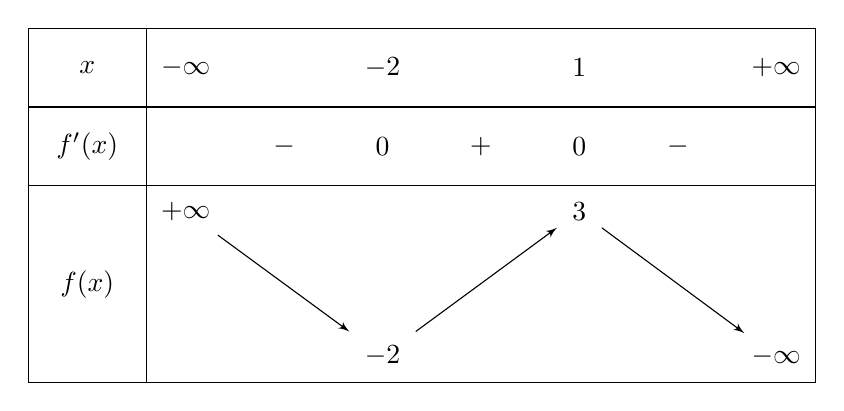
\begin{tikzpicture}
    \tkzTabInit[lgt=1.5, espcl=2.5]
    {$x$ /1, $f'(x)$ /1, $f(x)$ /2.5}
    {$-\infty$, $-2$, $1$, $+\infty$}
    \tkzTabLine{, -, 0, +, 0, - }
    \tkzTabVar{+/ $+\infty$ / , -/ $-2$ / , +/ $3$ / ,-/ $-\infty$ /}
\end{tikzpicture}
\end{center}

Hàm số \( y = f(x) \) đồng biến trên khoảng nào sau đây?}{
    \begin{tasks}(4)
        \task $(1; +\infty)$
        \task $(-2; 1)$
        \task $(-2; 3)$
        \task $(-\infty; -2)$
    \end{tasks}
}

% --- CÂU 56 ---
\questionLinesManual{0}{56}{Cho hàm số \( y = f(x) \) xác định trên \( \mathbb{R} \setminus \{-1\} \), liên tục trên mỗi khoảng xác định và có bảng biến thiên như hình:

\begin{center}
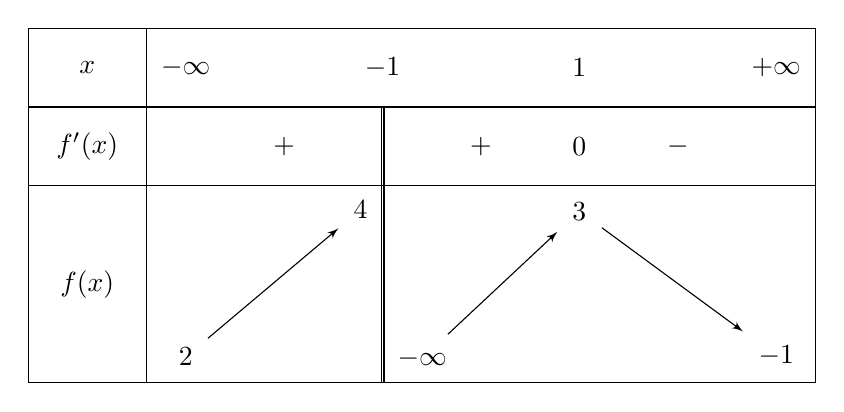
\begin{tikzpicture}
    \tkzTabInit[lgt=1.5, espcl=2.5]
    {$x$ /1, $f'(x)$ /1, $f(x)$ /2.5}
    {$-\infty$, $-1$, $1$, $+\infty$}
    \tkzTabLine{, +, d, +, 0, -, }
    \tkzTabVar{-/ $2$ / , +D-/ $4$ / $-\infty$, +/ $3$ / , -/ $-1$ /}
\end{tikzpicture}
\end{center}

Hỏi đồ thị hàm số có bao nhiêu đường tiệm cận ngang?}{
    \begin{tasks}(4)
        \task $1$
        \task $2$
        \task $0$
        \task $3$
    \end{tasks}
}

% --- CÂU 57 ---
\questionLinesManual{0}{57}{Hàm số nào dưới đây có đồ thị là đường cong như hình vẽ

\begin{center}
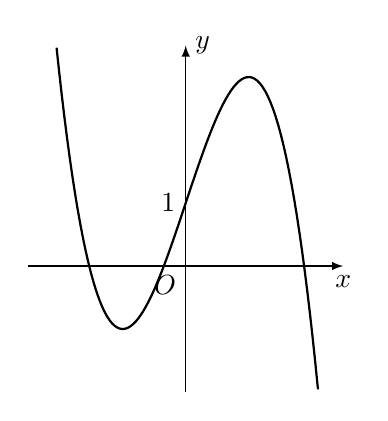
\begin{tikzpicture}[>=latex, scale=0.8]
    % Vẽ hệ trục
    \draw[->] (-2.5,0) -- (2.5,0) node[below] {$x$};
    \draw[->] (0,-2) -- (0,3.5) node[right] {$y$};
    \node[below left] at (0,0) {$O$};
    
    % Đánh dấu các mốc
    
    \foreach \y in {1} {
        \draw (0.01,\y) -- (-0.01,\y) node[left] {$\y$};
    }
    
    % Vẽ đồ thị hàm bậc 3
    \draw[thick, samples=100, domain=-2.05:2.1] 
        plot (\x, {-\x^3 + 3*\x + 1});
    
\end{tikzpicture}
\end{center}

}{
    \begin{tasks}(4)
        \task \( y = -x^4 + 3x + 1 \)
        \task \( y = x^3 - 3x + 1 \)
        \task \( y = -x^2 + 3x + 1 \)
        \task \( y = -x^3 + 3x + 1 \)
    \end{tasks}
}
% --- CÂU 58 ---
\questionLinesManual{0}{58}{Cho hàm số \( y = f(x) \) có bảng biến thiên sau:

\begin{center}
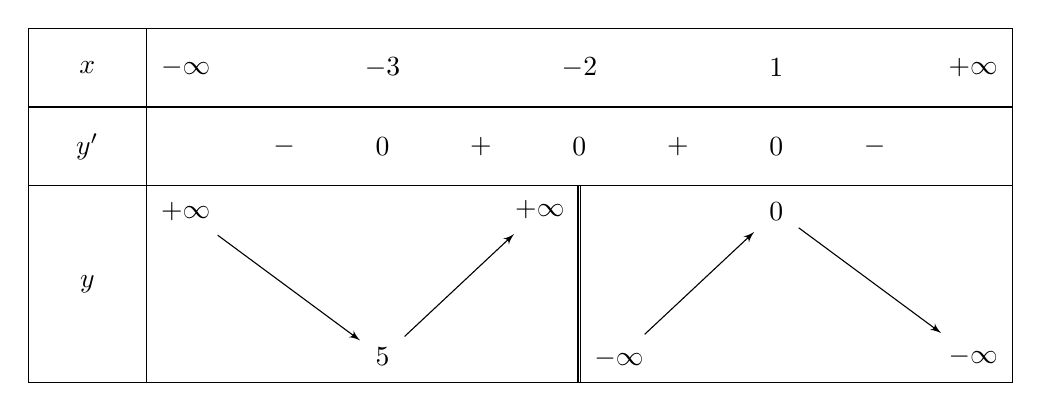
\begin{tikzpicture}
    \tkzTabInit[lgt=1.5, espcl=2.5]
    {$x$ /1, $y'$ /1, $y$ /2.5}
    {$-\infty$, $-3$, $-2$, $1$, $+\infty$}
    \tkzTabLine{, -, 0, +, 0, +, 0, -, }
    \tkzTabVar{+/ $+\infty$ / , -/ $5$ / , +D-/ $+\infty$ / $-\infty$, +/ $0$ / , -/ $-\infty$ /}
\end{tikzpicture}
\end{center}

Giá trị cực đại của hàm số \( y = f(x) \) là:}{
    \begin{tasks}(4)
        \task $1$
        \task $5$
        \task $0$
        \task $-3$
    \end{tasks}
}

% --- CÂU 59 ---
\questionLinesManual{0}{59}{Cho hàm số \( y = \dfrac{2x - 2}{x + 2} \) có tập xác định là \( D \). Hàm số đã cho có đạo hàm trên \( D \) là}{
    \begin{tasks}(4)
        \task \( y' = -\dfrac{2}{(x+2)^2} \)
        \task \( y' = \dfrac{6}{(x+2)^2} \)
        \task \( y' = \dfrac{2}{(x+2)^2} \)
        \task \( y' = -\dfrac{6}{(x+2)^2} \)
    \end{tasks}
}


% --- CÂU 60 ---
\questionLinesManual{0}{60}{Cho hàm số \( y = f(x) \) có đồ thị như hình vẽ

\begin{center}
\begin{tikzpicture}[>=latex, scale=0.8]
    % Vẽ hệ trục
    \draw[->] (-5.5,0) -- (3.5,0) node[below] {$x$};
    \draw[->] (0,-2.5) -- (0,6.5) node[right] {$y$};
    \node[below left] at (0,0) {$O$};
    \foreach \x in {-1} {
        \draw (\x,0.01) -- (\x,-0.01) node[below] {$\x$};
    }
    \foreach \y in {2} {
        \draw (0.01,\y) -- (-0.01,\y) node[left] {$\y$};
    }
    % Vẽ đồ thị hàm số
    \draw[thick, samples=100, domain=-5.5:-1.7] 
        plot (\x, {(2*\x - 1)/(\x + 1)});
    \draw[thick, samples=100, domain=-0.35:3.5] 
        plot (\x, {(2*\x - 1)/(\x + 1)});
    
    % Đường tiệm cận
    \draw[dashed] (-1,-2.5) -- (-1,6.5);
    \draw[dashed] (-5.5,2) -- (3.5,2);
    \
\end{tikzpicture}
\end{center}

Đồ thị hàm số đã cho có đường tiệm cận ngang là}{
    \begin{tasks}(4)
        \task \( x = 1 \)
        \task \( y = 2 \)
        \task \( y = 1 \)
        \task \( y = 3 \)
    \end{tasks}
}

% --- CÂU 61 ---
\questionLinesManual{0}{61}{Cho hàm số \( y = f(x) \) có đồ thị như hình vẽ

\begin{center}
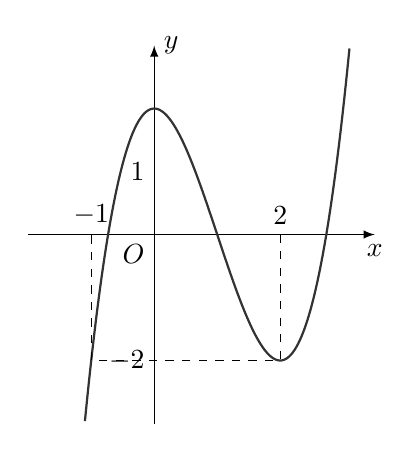
\begin{tikzpicture}[>=latex, scale=0.8]
    % Hệ trục tọa độ
    \draw[->] (-2,0) -- (3.5,0) node[below] {$x$};
    \draw[->] (0,-3) -- (0,3) node[right] {$y$};
    \node[below left] at (0,0) {$O$};
    
    % Đánh dấu các điểm
    \node[above] at (-1,0) {$-1$};
    \node[above] at (2,0) {$2$};
    \node[left] at (0,-2) {$-2$};
    \node[left] at (0,1) {$1$};
    
    % Vẽ đồ thị hàm bậc 3 y = x^3 - 3x^2 + 1
    \draw[thick, color=black!80, samples=150, domain=-1.1:3.1] 
        plot (\x, {\x*\x*\x - 3*\x*\x + 2});
    
    % Đường nét đứt
    \draw[dashed] (2,0) -- (2,-2) -- (-1,-2) -- (-1,0);
\end{tikzpicture}
\end{center}

Điểm cực đại của hàm số đã cho}{
    \begin{tasks}(4)
        \task \( x = 1 \)
        \task \( x = 2 \)
        \task \( x = 0 \)
        \task \( x = -2 \)
    \end{tasks}
}

% --- CÂU 62 ---
\questionLinesManual{0}{62}{Trong các hàm số cho dưới đây, hàm số nào đồng biến trên \((-\infty; +\infty)\)?}{
    \begin{tasks}(4)
        \task \( y = -x^3 + 3x + 1 \)
        \task \( y = 2x^3 + x - 5 \)
        \task \( y = \sqrt{x} \)
        \task \( y = \dfrac{2x - 1}{x + 1} \)
    \end{tasks}
}

% --- CÂU 63 ---
\questionLinesManual{0}{63}{Cho hàm số \( y = f(x) \) liên tục trên đoạn \([1; 5]\) và có đồ thị như hình vẽ sau.

\begin{center}
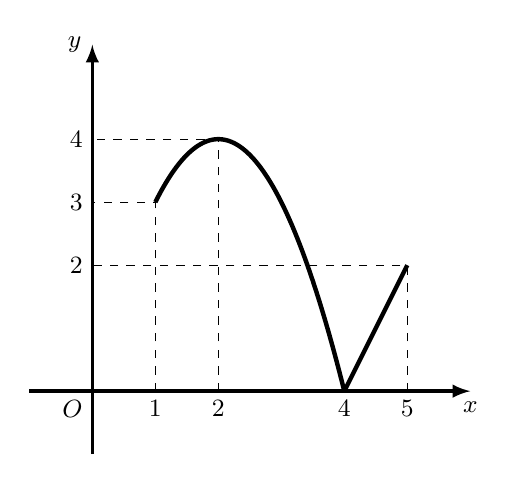
\begin{tikzpicture}[>=latex, scale=0.8]
    % 1. Hệ trục tọa độ Ox, Oy dày và rõ nét
    \draw[->, line width=1.2pt] (-1,0) -- (6,0) node[below] {\small $x$};
    \draw[->, line width=1.2pt] (0,-1) -- (0,5.5) node[left] {\small $y$};
    \node[below left] at (0,0) {\small $O$};
    
    % 2. Đồ thị hàm số từng nhánh
    % Nhánh 1: Parabol từ x = 1 (y = 3) đạt cực đại tại đỉnh x = 2 (y = 4) xuôi xuống x = 4 (y = 0)
    % Hàm phù hợp: y = -(x-2)^2 + 4
    \draw[ultra thick, samples=150, domain=1:4] plot (\x, {-(\x-2)*(\x-2) + 4});
    % Nhánh 2: Đoạn thẳng từ (4, 0) lên (5, 2)
    \draw[ultra thick] (4,0) -- (5,2);

    % 3. Đường nét đứt và điền số trục tọa độ
    % Tại x = 1, y = 3
    \draw[dashed] (1,0) -- (1,3) -- (0,3);
    \node[below] at (1,0) {\small $1$};
    \node[left] at (0,3) {\small $3$};
    
    % Tại x = 2, y = 4 (Đỉnh)
    \draw[dashed] (2,0) -- (2,4) -- (0,4);
    \node[below] at (2,0) {\small $2$};
    \node[left] at (0,4) {\small $4$};
    
    % Tại x = 4, y = 0
    \node[below] at (4,0) {\small $4$};
    
    % Tại x = 5, y = 2
    \draw[dashed] (5,0) -- (5,2) -- (0,2);
    \node[below] at (5,0) {\small $5$};
    \node[left] at (0,2) {\small $2$};

\end{tikzpicture}
\end{center}

Trên đoạn \([1; 5]\), hàm số đã cho đạt giá trị lớn nhất tại điểm.}{
    \begin{tasks}(4)
        \task \( x = 1 \)
        \task \( x = 4 \)
        \task \( x = 5 \)
        \task \( x = 2 \)
    \end{tasks}
}

% --- CÂU 64 ---
\questionLinesManual{0}{64}{Cho hàm số bậc ba \( y = f(x) \) có đồ thị đạo hàm \( y = f'(x) \) như hình sau

\begin{center}
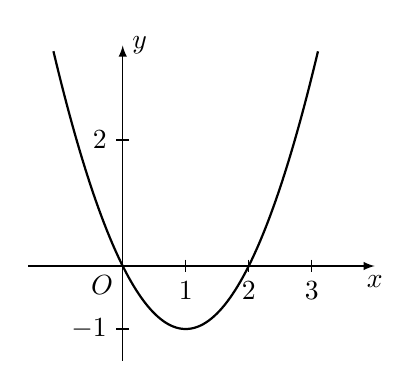
\begin{tikzpicture}[>=latex, scale=0.8]
    % Vẽ hệ trục
    \draw[->] (-1.5,0) -- (4,0) node[below] {$x$};
    \draw[->] (0,-1.5) -- (0,3.5) node[right] {$y$};
    \node[below left] at (0,0) {$O$};
    
    % Đánh dấu các mốc
    \foreach \x in {1,2,3} {
        \draw (\x,0.1) -- (\x,-0.1) node[below] {$\x$};
    }
    \foreach \y in {-1,2} {
        \draw (0.1,\y) -- (-0.1,\y) node[left] {$\y$};
    }
    
    % Vẽ đồ thị f'(x)
    \draw[thick, samples=100, domain=-1.1:3.1] 
        plot (\x, {(\x)*(\x-2)});
    
    
\end{tikzpicture}
\end{center}

Hàm số đã cho nghịch biến trên khoảng}{
    \begin{tasks}(4)
        \task $(-1; 0)$
        \task $(2; 3)$
        \task $(1; 2)$
        \task $(3; 4)$
    \end{tasks}
}

% --- CÂU 65 ---
\questionLinesManual{0}{65}{Giá trị lớn nhất của hàm số \( y = x^3 - 3x \) trên đoạn \([0; 3]\) bằng}{
    \begin{tasks}(4)
        \task $0$
        \task $2$
        \task $18$
        \task $-2$
    \end{tasks}
}

% --- CÂU 66 ---
\questionLinesManual{0}{66}{Trong hệ trục tọa độ \( Oxy \), tiệm cận ngang của đồ thị hàm số \( y = \dfrac{2}{x-2} \) có phương trình là:}{
    \begin{tasks}(4)
        \task \( y = 2 \)
        \task \( y = -1 \)
        \task \( y = 0 \)
        \task \( x = 2 \)
    \end{tasks}
}

% --- CÂU 67 ---
\questionLinesManual{0}{67}{Cho hàm số \( y = f(x) \) có một phần đồ thị như hình bên.

\begin{center}
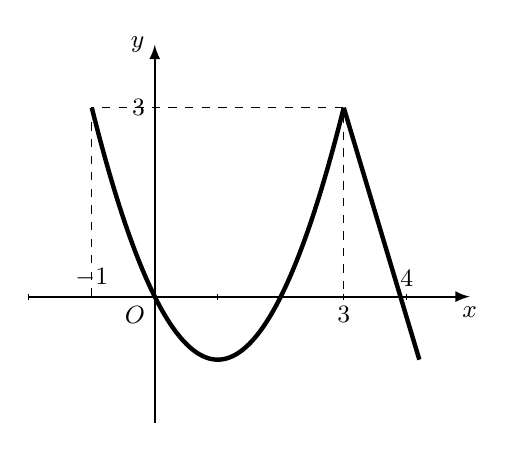
\begin{tikzpicture}[>=latex, scale=0.8]
    % 1. Hệ trục tọa độ Ox, Oy màu đen
    \draw[->, black, thick] (-2,0) -- (5,0) node[below] {\small $x$};
    \draw[->, black, thick] (0,-2) -- (0,4) node[left] {\small $y$};
    \node[below left] at (0,0) {\small $O$};

    % Các vạch nhỏ chia tọa độ trên trục Ox và Oy
    \foreach \x in {-2, 1, 3, 4} \draw[black] (\x, 0.05) -- (\x, -0.05);
    \draw[black, ultra thick, samples=150, domain=-1:3] plot (\x, {(\x)*(\x-2)});
    
    % Nhánh 2: Đoạn thẳng dốc xuống từ cực đại nhọn (3, 2) đến điểm mút (4, -4)
    \draw[black, ultra thick] (3,3) -- (4.2,-1);

    \draw[dashed, black] (-1,0) -- (-1,3) -- (3,3) -- (3,0);
     \node[above] at (-1,0) {\small $-1$};
    \node[below] at (3,0) {\small $3$};
    \node[left] at (0,3) {\small $3$};
 
    \node[above] at (4,0) {\small $4$};
 

\end{tikzpicture}
\end{center}
Khoảng đồng biến của hàm số \( y = f(x) \) là:}{
    \begin{tasks}(4)
        \task $(2; 4)$
        \task $(0; 3)$
        \task $(-1; 0)$
        \task $(1; 3)$
    \end{tasks}
}

% --- CÂU 68 ---
\questionLinesManual{0}{68}{Đường cong ở hình bên là đồ thị của hàm số nào sau đây?

\begin{center}
\begin{tikzpicture}[>=latex, scale=0.8]
    % 1. Hệ trục tọa độ
    \draw[->] (-4.5,0) -- (4.5,0) node[below] {\small $x$};
    \draw[->] (0,-4.5) -- (0,4.5) node[right] {\small $y$};
    \node[below left] at (0,0) {\small $O$};
    
    % 2. Đánh dấu các mốc
    \foreach \x in {-1} {
        \draw (\x,0.05) -- (\x,-0.05) node[below] {\tiny $\x$};
    }
    \foreach \val in {-2,-1} {
        \draw (0.05,\val) -- (-0.05,\val) node[left] {\tiny $\val$};
    }
    
    % 3. Vẽ đồ thị hàm số y = (x^2 + 2x + 2)/(x + 1)
    \draw[thick, samples=100, domain=-5:-1.23] 
        plot (\x, {-(\x*\x + 2*\x + 2)/(\x + 1)});
    \draw[thick, samples=100, domain=-0.77:3] 
        plot (\x, {-(\x*\x + 2*\x + 2)/(\x + 1)});
    \draw[thick, samples=100, domain=-5:3] 
        plot (\x, {-\x-1});
    
    % 4. Đường tiệm cận
    \draw[thick] (-1,-4.5) -- (-1,4.5);
\end{tikzpicture}
\end{center}

}{
    \begin{tasks}(4)
        \task \( y = \dfrac{-x^2 - 2x - 2}{x + 1} \)
        \task \( y = \dfrac{x^2 + 2x + 2}{x - 1} \)
        \task \( y = \dfrac{-x^2 - 2x}{x + 1} \)
        \task \( y = \dfrac{x^2 - 2x + 2}{x + 1} \)
    \end{tasks}
}

% --- CÂU 69 ---
\questionLinesManual{0}{69}{Đồ thị hàm số \( y = \dfrac{2x - 3}{x - 1} \) có đường tiệm cận ngang là}{
    \begin{tasks}(4)
        \task \( x = -1 \)
        \task \( y = -2 \)
        \task \( x = 1 \)
        \task \( y = 2 \)
    \end{tasks}
}

% --- CÂU 70 ---
\questionLinesManual{0}{70}{Cho hàm số \( y = f(x) = ax^4 + bx^3 + cx^2 + dx + e \) có đạo hàm \( f'(x) \) và đồ thị hàm số \( y = f'(x) \) cắt trục hoành tại các điểm có hoành độ \(-1; 0; 2\) như hình bên. Hỏi hàm số \( y = f(x) \) đồng biến trên khoảng nào sau đây?

\begin{center}
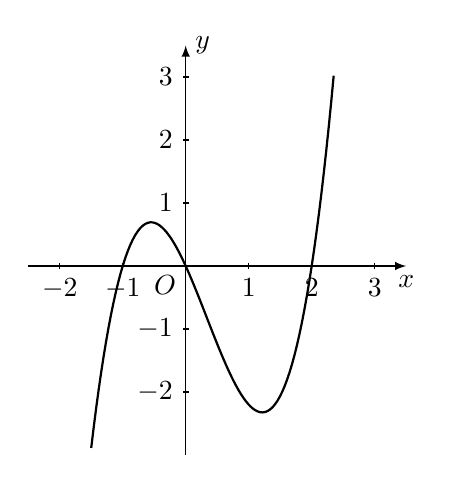
\begin{tikzpicture}[>=latex, scale=0.8]
    % Vẽ hệ trục
    \draw[->] (-2.5,0) -- (3.5,0) node[below] {$x$};
    \draw[->] (0,-3) -- (0,3.5) node[right] {$y$};
    \node[below left] at (0,0) {$O$};
    
    % Đánh dấu các mốc
    \foreach \x in {-2,-1,1,2,3} {
        \draw (\x,0.05) -- (\x,-0.05) node[below] {$\x$};
    }
    \foreach \y in {-2,-1,1,2,3} {
        \draw (0.05,\y) -- (-0.05,\y) node[left] {$\y$};
    }
    
    % Vẽ đồ thị f'(x)
    \draw[thick, samples=100, domain=-1.5:2.35] 
        plot (\x, {1.1*(\x+1)*\x*(\x-2)});
\end{tikzpicture}
\end{center}

}{
    \begin{tasks}(4)
        \task $(-\infty; -1)$
        \task $(1; +\infty)$
        \task $(0; 2)$
        \task $(-1; 0)$
    \end{tasks}
}

% --- CÂU 71 ---
\questionLinesManual{0}{71}{Tính đạo hàm của hàm số \( y = e^x + \log x \).}{
    \begin{tasks}(4)
        \task \( y' = e^x - \dfrac{1}{x\ln 10} \)
        \task \( y' = e^x + \dfrac{1}{x} \)
        \task \( y' = e^x + \dfrac{1}{x\ln 10} \)
        \task \( y' = e^x - \dfrac{1}{x} \)
    \end{tasks}
}

% --- CÂU 72 ---
\questionLinesManual{0}{72}{Cho hàm số \( f(x) \) xác định và có đạo hàm trên \( \mathbb{R} \) và có bảng biến thiên như sau:

\begin{center}
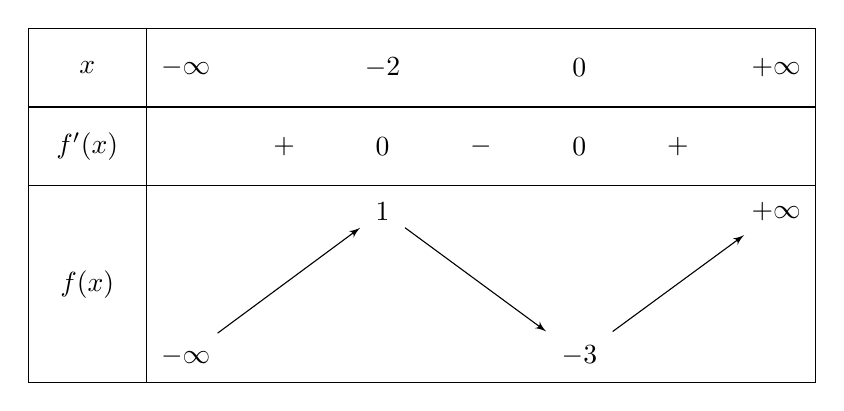
\begin{tikzpicture}
    \tkzTabInit[lgt=1.5, espcl=2.5]
    {$x$ /1, $f'(x)$ /1, $f(x)$ /2.5}
    {$-\infty$, $-2$, $0$, $+\infty$}
    \tkzTabLine{, +, 0, -,0,+ }
    \tkzTabVar{-/ $-\infty$ / , +/ $1$ / , -/ $-3$ / , +/ $+\infty$ /}
\end{tikzpicture}
\end{center}

Giá trị cực đại của hàm số bằng}{
    \begin{tasks}(4)
        \task $-2$
        \task $0$
        \task $-3$
        \task $1$
    \end{tasks}
}

% --- CÂU 73 ---
\questionLinesManual{0}{73}{Cho hàm số \( y = f(x) \) có bảng biến thiên như hình vẽ dưới đây. Hàm số đã cho nghịch biến trên khoảng

\begin{center}
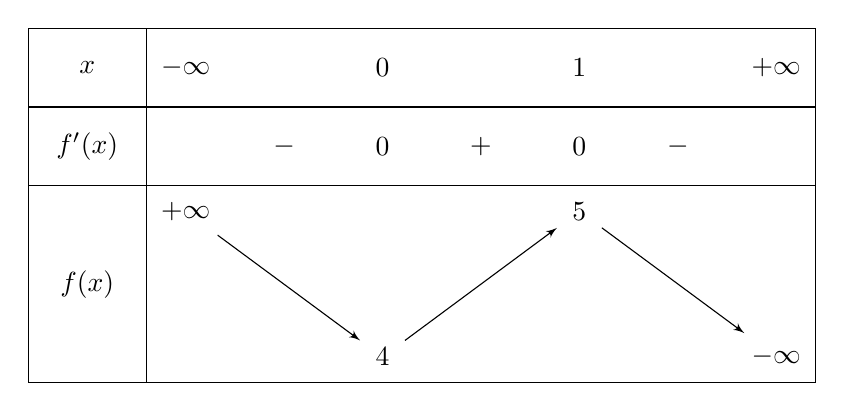
\begin{tikzpicture}
    \tkzTabInit[lgt=1.5, espcl=2.5]
    {$x$ /1, $f'(x)$ /1, $f(x)$ /2.5}
    {$-\infty$, $0$, $1$, $+\infty$}
    \tkzTabLine{, -, 0, +, 0, -, }
    \tkzTabVar{+/ $+\infty$ / , -/ $4$ / , +/ $5$ / , -/ $-\infty$ /}
\end{tikzpicture}
\end{center}

}{
    \begin{tasks}(4)
        \task $(0; +\infty)$
        \task $(-\infty; 0)$
        \task $(0; 1)$
        \task $(-\infty; 5)$
    \end{tasks}
}

% --- CÂU 74 ---
\questionLinesManual{0}{74}{Cho hàm số bậc ba \( y = f(x) \) có bảng biến thiên như sau. Điểm cực tiểu của đồ thị hàm số là:

\begin{center}
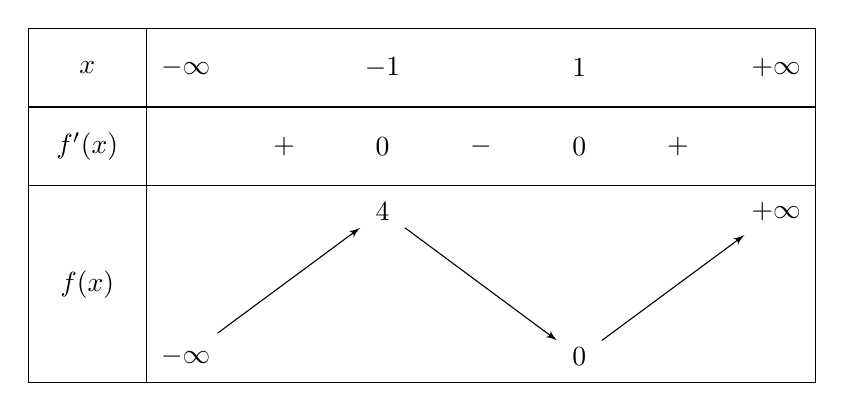
\begin{tikzpicture}
    \tkzTabInit[lgt=1.5, espcl=2.5]
    {$x$ /1, $f'(x)$ /1, $f(x)$ /2.5}
    {$-\infty$, $-1$, $1$, $+\infty$}
    \tkzTabLine{, +, 0, -, 0, +, }
    \tkzTabVar{-/ $-\infty$ / , +/ $4$ / , -/ $0$ / , +/ $+\infty$ /}
\end{tikzpicture}
\end{center}

}{
    \begin{tasks}(4)
        \task $(-1; 0)$
        \task $(1; 0)$
        \task $(-1; 4)$
        \task $(1; 4)$
    \end{tasks}
}

% --- CÂU 75 ---
\questionLinesManual{0}{75}{Cho hàm số \( y = f(x) \) liên tục trên đoạn \([-1; 3]\) và có đồ thị như hình vẽ. Giá trị lớn nhất của hàm số đã cho trên đoạn \([-1; 3]\) bằng

\begin{center}
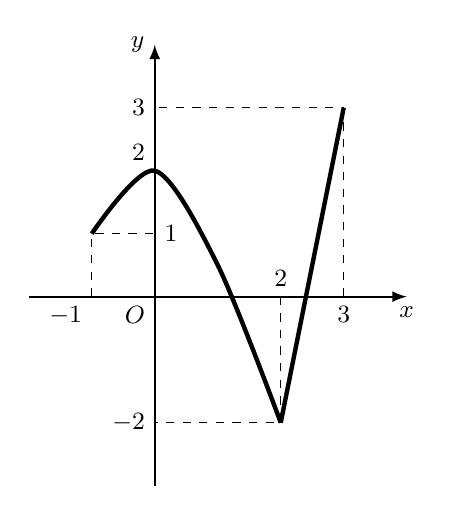
\begin{tikzpicture}[>=latex, scale=0.8]
    % 1. Hệ trục tọa độ Ox, Oy màu đen
    \draw[->, black, thick] (-2,0) -- (4,0) node[below] {\small $x$};
    \draw[->, black, thick] (0,-3) -- (0,4) node[left] {\small $y$};
    \node[below left] at (0,0) {\small $O$};
    \draw[black, ultra thick, samples=100] plot[smooth, domain=-1:2] coordinates {(-1,1) (0,2) (1,0.5) (2,-2)};
    
    % Nhánh phải: đoạn thẳng từ cực tiểu (2, -2) lên điểm mút (3, 3)
    \draw[black, ultra thick] (2,-2) -- (3,3);

    % 3. Các đường nét đứt và nhãn tọa độ màu đen
    % Tại điểm đầu mút x = -1, y = 1
    \draw[dashed, black] (-1,0) -- (-1,1) -- (0,1);
    \node[below left] at (-1,0) {\small $-1$};
    \node[right] at (0,1) {\small $1$};
    
    % Tại điểm cực đại y = 2 trên trục Oy
    \node[above left] at (0,2) {\small $2$};
    
    % Tại cực tiểu x = 2, y = -2
    \draw[dashed, black] (2,0) -- (2,-2) -- (0,-2);
    \node[above] at (2,0) {\small $2$};
    \node[left] at (0,-2) {\small $-2$};
    
    % Tại điểm đầu mút x = 3, y = 3
    \draw[dashed, black] (3,0) -- (3,3) -- (0,3);
    \node[below] at (3,0) {\small $3$};
    \node[left] at (0,3) {\small $3$};

\end{tikzpicture}
\end{center}

}{
    \begin{tasks}(4)
        \task $2$
        \task $0$
        \task $1$
        \task $3$
    \end{tasks}
}

% --- CÂU 76 ---
\questionLinesManual{0}{76}{Hàm số \( y = \dfrac{ax + b}{cx + d} \) (\( c \neq 0, ad - bc \neq 0 \)) có đồ thị dưới đây. Đường tiệm cận đứng của đồ thị hàm số là:

\begin{center}
\begin{tikzpicture}[>=latex, scale=0.8]
    % 2. Vẽ hệ trục tọa độ
    \draw[->] (-3.5,0) -- (5,0) node[below] {\small$x$};
    \draw[->] (0,-3.5) -- (0,5) node[right] {\small $y$};
    \node[below left] at (0,0) {\small $O$};
    % 4. Vẽ đồ thị hàm số y = (2x-1)/(x-1)
    \draw[thick, samples=100, domain=-3.5:0.55] 
        plot (\x, {(\x + 1)/(\x - 1)});
    \draw[thick, samples=100, domain=1.5:5] 
        plot (\x, {(\x + 1)/(\x - 1)});
    
    % 5. Đường tiệm cận
    \draw[thick] (1,-3.5) -- (1,5) ;
    \draw[thick] (-3.5,1) -- (5,1) ;
    \node [below right] at (1,0) {\small$1$};
    \node [below left] at (0,1) {\small $1$};
    
\end{tikzpicture}
\end{center}

}{
    \begin{tasks}(4)
        \task \( x = -1 \)
        \task \( x = 1 \)
        \task \( x = 2 \)
        \task \( y = 1 \)
    \end{tasks}
}

% --- CÂU 77 ---
\questionLinesManual{0}{77}{Đồ thị nào dưới đây có dạng đường cong như hình bên?

\begin{center}
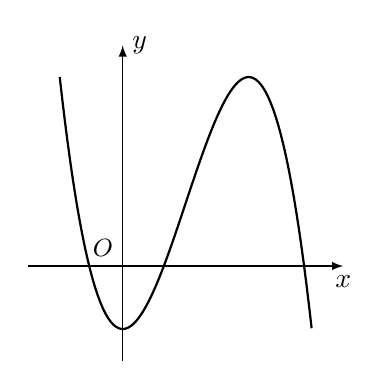
\begin{tikzpicture}[>=latex, scale=0.8]
    % Vẽ hệ trục
    \draw[->] (-1.5,0) -- (3.5,0) node[below] {$x$};
    \draw[->] (0,-1.5) -- (0,3.5) node[right] {$y$};
    \node[above left] at (0,0) {\small$O$};
    
    
    % Vẽ đồ thị hàm số
    \draw[thick, samples=100, domain=-1:3] 
        plot (\x, {-\x*\x*\x +3*\x*\x-1});
   
\end{tikzpicture}
\end{center}

}{
    \begin{tasks}(4)
        \task \( y = x^3 - 3x^2 - 1 \)
        \task \( y = \dfrac{x^3 - 3x + 1}{x - 1} \)
        \task \( y = -x^3 + 3x^2 - 1 \)
        \task \( y = \dfrac{x + 1}{x - 1} \)
    \end{tasks}
}

% --- CÂU 78 ---
\questionLinesManual{0}{78}{Cho hàm số \( y = \dfrac{ax + b}{cx + d} \) có đồ thị là đường cong như hình vẽ bên. Tọa độ giao điểm của đồ thị hàm số với trục hoành là
\begin{center}
\begin{tikzpicture}[>=latex, scale=0.8]
    % Hệ trục tọa độ
    \draw[->] (-3.5,0) -- (5.5,0) node[below] {\small $x$};
    \draw[->] (0,-3.5) -- (0,5.5) node[right] {\small $y$};
    \node[below left] at (0,0) {\small $O$};
    
    % Đánh dấu các mốc
    \foreach \x in {1,2} {
        \draw (\x,0.05) -- (\x,-0.05) node[below right] {\small $\x$};
    }
    \foreach \val in {1,2} {
        \draw (0.05,\val) -- (-0.05,\val) node[ above left] {\small$\val$};
    }
    
    % Vẽ đồ thị hàm số y = (x+1)/(x-1)
    \draw[thick, samples=100, domain=-3.5:0.77] 
        plot (\x, {(\x -2)/(\x - 1)});
    \draw[thick, samples=100, domain=1.23:5.5] 
        plot (\x, {(\x -2)/(\x - 1)});
    
    % Đường tiệm cận
    \draw[thick] (1,-3.5) -- (1,5.5) ;
    \draw[thick] (-3.5,1) -- (5.5,1) ;
    
\end{tikzpicture}
\end{center}

}{
    \begin{tasks}(4)
        \task $(2; 0)$
        \task $(0; 1)$
        \task $(1; 0)$
        \task $(0; 2)$
    \end{tasks}
}

% --- CÂU 79 ---
\questionLinesManual{0}{79}{Trong 5 giây đầu tiên, một chất điểm chuyển động theo phương trình \( S(t) = -t^3 + 6t^2 + t + 5 \) trong đó \( t \) tính bằng giây và \( S(t) \) tính bằng mét. Tính vận tốc của vật tại thời điểm \( t = 3 \) giây.}{
    \begin{tasks}(4)
        \task $35$ m/s
        \task $10$ m/s
        \task $64$ m/s
        \task $13$ m/s
    \end{tasks}
}

% --- CÂU 80 ---
\questionLinesManual{0}{80}{Cho hàm số \( f(x) \) có bảng biến thiên sau. Hàm số đã cho có điểm cực đại là

\begin{center}
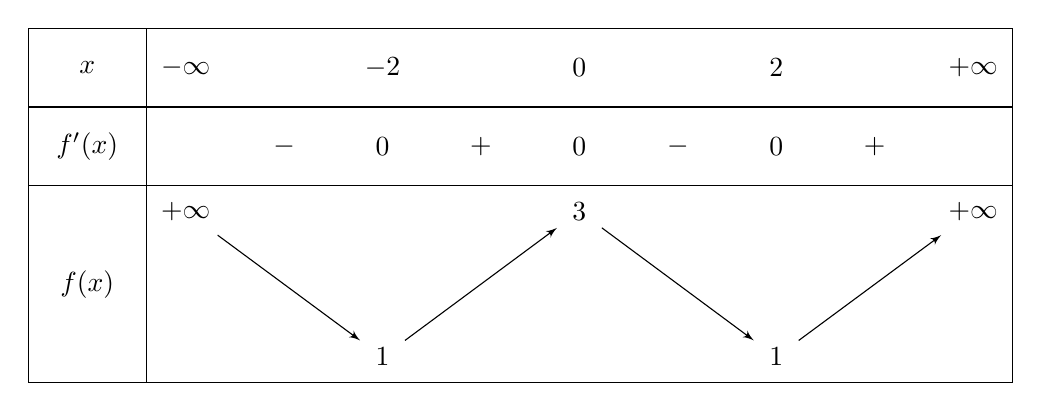
\begin{tikzpicture}
    \tkzTabInit[lgt=1.5, espcl=2.5]
    {$x$ /1, $f'(x)$ /1, $f(x)$ /2.5}
    {$-\infty$, $-2$, $0$, $2$, $+\infty$}
    \tkzTabLine{, -, 0, +, 0, -, 0, +, }
    \tkzTabVar{+/ $+\infty$ / , -/ $1$ / , +/ $3$ / , -/ $1$ / , +/ $+\infty$ /}
\end{tikzpicture}
\end{center}

}{
    \begin{tasks}(4)
        \task $(0;3)$
        \task $x = 0$
        \task $y = 3$
        \task $y = 1$
    \end{tasks}
}

% --- CÂU 81 ---
\questionLinesManual{0}{81}{Hàm số \( y = \sqrt{-x^2 + 2x} \) đồng biến trên khoảng nào?}{
    \begin{tasks}(4)
        \task $(0;1)$
        \task $(1;2)$
        \task $(-\infty;0)$
        \task $(2;+\infty)$
    \end{tasks}
}

% --- CÂU 82 ---
\questionLinesManual{0}{82}{Cho hàm số \( y = \dfrac{x^2 - 3x + 4}{x+1} \). Tiệm cận đứng của đồ thị hàm số là}{
    \begin{tasks}(4)
        \task $y = 1$
        \task $x = -1$
        \task $x = 1$
        \task $y = -1$
    \end{tasks}
}

% --- CÂU 83 ---
\questionLinesManual{0}{83}{Cho hàm số \( y = f(x) \) liên tục trên \( \mathbb{R} \), có bảng xét dấu đạo hàm như sau.

\begin{center}
\begin{tikzpicture}
    \tkzTabInit[lgt=1.5, espcl=2.5]
    {$x$ /1, $f'(x)$ /1}
    {$-\infty$, $-2$, $0$, $2$, $+\infty$}
    \tkzTabLine{, +, 0, -, d, -, 0, +, }
    
\end{tikzpicture}
\end{center}

Khẳng định nào dưới đây đúng?}{
    \begin{tasks}(2)
        \task Hàm số nghịch biến trên khoảng \( (-\infty; 0) \).
        \task Hàm số đồng biến trên khoảng \( (1; +\infty) \).
        \task Hàm số đồng biến trên khoảng \( (-\infty; -2) \).
        \task Hàm số nghịch biến trên khoảng \( (0; 4) \).
    \end{tasks}
}

% --- CÂU 84 ---
\questionLinesManual{0}{84}{Giá trị lớn nhất của hàm số \( y = x^3 - 3x + 2 \) trên đoạn \([0; 3]\) bằng}{
    \begin{tasks}(4)
        \task $2$
        \task $3$
        \task $20$
        \task $0$
    \end{tasks}
}

% --- CÂU 85 ---
\questionLinesManual{0}{85}{Cho hàm số \( y = f(x) \) có bảng biến thiên như hình vẽ sau:

\begin{center}
\begin{tikzpicture}
    \tkzTabInit[lgt=1.5, espcl=2.5]
    {$x$ /1, $f'(x)$ /1, $f(x)$ /2.5}
    {$-\infty$, $-1$, $1$, $3$, $+\infty$}
    \tkzTabLine{, -, d, +, d, -, 0, +, }
    \tkzTabVar{+/ $+\infty$ / , -D-/ $-\infty$ / $-2$, +D+/ $4$ / $1$ / , -/ $-5$, +/$0$ /}
\end{tikzpicture}
\end{center}

Tổng số đường tiệm cận đứng và tiệm cận ngang của đồ thị hàm số \( y = f(x) \) là}{
    \begin{tasks}(4)
        \task $3$
        \task $1$
        \task $4$
        \task $2$
    \end{tasks}
}

% --- CÂU 86 ---
\questionLinesManual{0}{86}{Cho hàm số bậc ba \( y = f(x) \) có đồ thị như hình vẽ sau

\begin{center}
\begin{tikzpicture}[>=latex, scale=0.8]
    % Vẽ hệ trục
    \draw[->] (-3.5,0) -- (3.5,0) node[below] {$x$};
    \draw[->] (0,-3.5) -- (0,3.5) node[right] {$y$};
    \node[below left] at (0,0) {$O$};
    
    % Đánh dấu các mốc
    \foreach \x in {-1,1} {
        \draw (\x,0.05) -- (\x,-0.05) node[below] {$\x$};
    }
    \foreach \y in {-2,2} {
        \draw (0.05,\y) -- (-0.05,\y) node[left] {$\y$};
    }
    
    % Vẽ đồ thị hàm bậc 3
    \draw[thick, samples=100, domain=-2.1:2.1] 
        plot (\x, {\x^3 - 3*\x});
    \draw[dashed] (-1,0) -- (-1,2) -- (0,2);
    \draw[dashed] (1,0) -- (1,-2) -- (0,-2);
    
\end{tikzpicture}
\end{center}

Giá trị cực đại của hàm số đã cho là}{
    \begin{tasks}(4)
        \task $1$
        \task $-1$
        \task $2$
        \task $-2$
    \end{tasks}
}

% --- CÂU 87 ---
\questionLinesManual{0}{87}{Phương trình đường tiệm cận xiên của đồ thị hàm số \( y = \dfrac{x^2 + x - 3}{x + 1} \) là}{
    \begin{tasks}(4)
        \task \( y = x + 1 \)
        \task \( y = x \)
        \task \( y = x - 3 \)
        \task \( y = 2x \)
    \end{tasks}
}

% --- CÂU 88 ---
\questionLinesManual{0}{88}{Đồ thị hàm số \( y = \dfrac{2x + 3}{x - 1} \) có tâm đối xứng là điểm}{
    \begin{tasks}(4)
        \task \( N(3; -1) \)
        \task \( P(1; 2) \)
        \task \( Q\left(1; -\dfrac{3}{2}\right) \)
        \task \( M(2; -1) \)
    \end{tasks}
}

% --- CÂU 89 ---
\questionLinesManual{0}{89}{Cho hàm số \( y = f(x) \) có bảng biến thiên như sau:

\begin{center}
\begin{tikzpicture}
    \tkzTabInit[lgt=1.5, espcl=2.5]
    {$x$ /1, $f'(x)$ /1, $f(x)$ /2.5}
    {$-\infty$, $-1$, $0$, $1$, $+\infty$}
    \tkzTabLine{,-,0, +, 0, -, 0, +}
    \tkzTabVar{+/ $+\infty$ / , -/ $-2$ / , +/ $3$ / , -/ $-2$ / , +/ $+\infty$ /}
\end{tikzpicture}
\end{center}

Hàm số đã cho nghịch biến trên khoảng nào dưới đây?}{
    \begin{tasks}(4)
        \task $(-1; 0)$
        \task $(-\infty; 0)$
        \task $(1; +\infty)$
        \task $(0; 1)$
    \end{tasks}
}

% --- CÂU 90 ---
\questionLinesManual{0}{90}{Cho hàm số \( f(x) \) có đồ thị như hình bên. Giá trị lớn nhất của hàm số \( f(x) \) trên đoạn \([-3; 2]\) đạt tại \( x \) bằng

\begin{center}
\begin{tikzpicture}[>=latex, scale=0.6]
    % Vẽ hệ trục
    \draw[->] (-3.5,0) -- (3.5,0) node[below] {$x$};
    \draw[->] (0,-2.5) -- (0,5) node[right] {$y$};
    \node[below left] at (0,0) {$O$};
    
    % Đánh dấu các mốc
    \foreach \x in {-3,3} {
        \draw (\x,0.1) -- (\x,-0.1) node[below] {$\x$};
    }
    \foreach \y in {-2,2,4} {
        \draw (0.1,\y) -- (-0.1,\y) node[above left] {$\y$};
    }
    
    % Vẽ đồ thị hàm số
    \draw[thick, samples=100, domain=-3.05:3.05] 
        plot (\x, {1/4*\x*\x*\x*\x-2*\x*\x+2});
    \draw[dashed] (-3,0) -- (-3,4) -- (3,4)-- (3,0);
    \draw[dashed] (-2,0) -- (-2,-2) -- (2,-2)-- (2,0);
\end{tikzpicture}
\end{center}

}{
    \begin{tasks}(4)
        \task $4$
        \task $2$
        \task $-3$
        \task $0$
    \end{tasks}
}

% --- CÂU 91 ---
\questionLinesManual{0}{91}{Tiệm cận đứng của đồ thị hàm số \( y = \dfrac{2x + 4}{x - 1} \) là}{
    \begin{tasks}(4)
        \task \( x = 1 \)
        \task \( x = -1 \)
        \task \( x = 2 \)
        \task \( x = -2 \)
    \end{tasks}
}

% --- CÂU 92 ---
\questionLinesManual{0}{92}{Hàm số nào dưới đây có đồ thị như đường cong trong hình bên?

\begin{center}
\begin{tikzpicture}[>=latex, scale=0.8]
    % Vẽ hệ trục
    \draw[->] (-3.5,0) -- (3.5,0) node[below] {$x$};
    \draw[->] (0,-3.5) -- (0,3.5) node[right] {$y$};
    \node[below right] at (0,0) {$O$};
    
    % Vẽ đồ thị hàm bậc 3
    \draw[thick, samples=100, domain=-2.05:2.2] 
        plot (\x, {\x^3 - 3*\x - 1});
\end{tikzpicture}
\end{center}

}{
    \begin{tasks}(4)
        \task \( y = \dfrac{x^2 - 2x + 3}{x - 1} \)
        \task \( y = \dfrac{x + 1}{x - 1} \)
        \task \( y = x^3 - 3x - 1 \)
        \task \( y = x^2 + x - 1 \)
    \end{tasks}
}

% --- CÂU 93 ---
\questionLinesManual{0}{93}{Hàm số nào dưới đây đơn điệu trên tập xác định của nó?}{
    \begin{tasks}(4)
        \task \( y = \sqrt{x^3 + x - 5} \)
        \task \( y = \dfrac{4x - 2}{x - 1} \)
        \task \( y = x^4 + x^3 + x + 11 \)
        \task \( y = \cot 2x \)
    \end{tasks}
}

% --- CÂU 94 ---
\questionLinesManual{0}{94}{Hình vẽ bên là đồ thị của hàm số \( y = \dfrac{ax + b}{cx + d} \). Đường tiệm cận đứng của đồ thị có phương trình là

\begin{center}
\begin{tikzpicture}[>=latex, scale=0.8]

    \draw[->] (-3.5,0) -- (5.5,0) node[below] {\small $x$};
    \draw[->] (0,-3.5) -- (0,5.5) node[right] {\small $y$};
    \node[below left] at (0,0) {\small $O$};
    % Vẽ đồ thị hàm số y = (x+1)/(x-1)
    \draw[thick, samples=100, domain=-3.5:0.65] 
        plot (\x, {(0.5*\x + 1)/(\x - 1)});
    \draw[thick, samples=100, domain=1.3:5.5] 
        plot (\x, {(0.5*\x + 1)/(\x - 1)});
    \node [below right] at (1,0) {\small$1$};
    \node [above left] at ( 0,0.5) {\small$\dfrac{1}{2}$};
    % Đường tiệm cận
    \draw[thick] (1,-3.5) -- (1,5.5);
    \draw[thick] (-3.5,0.5) -- (5.5,0.5);
    
\end{tikzpicture}
\end{center}

}{
    \begin{tasks}(4)
        \task \( x = 1 \)
        \task \( x = \dfrac{1}{2} \)
        \task \( y = 1 \)
        \task \( y = \dfrac{1}{2} \)
    \end{tasks}
}

% --- CÂU 95 ---
\questionLinesManual{0}{95}{Tìm giá trị lớn nhất của hàm số \( y = \dfrac{2x - 1}{x + 1} \) trên đoạn \([1; 2]\).}{
    \begin{tasks}(4)
        \task \( \max_{[1; 2]} y = \dfrac{1}{2} \)
        \task \( \max_{[1; 2]} y = -\dfrac{1}{2} \)
        \task \( \max_{[1; 2]} y = -\dfrac{1}{3} \)
        \task \( \max_{[1; 2]} y = 1 \)
    \end{tasks}
}

% --- CÂU 96 ---
\questionLinesManual{0}{96}{Tiệm cận xiên của đồ thị hàm số \( y = \dfrac{-x^2 - 2x + 5}{x + 2} \) là}{
    \begin{tasks}(4)
        \task \( y = -x \)
        \task \( y = -x + 1 \)
        \task \( y = x + 2 \)
        \task \( x = -2 \)
    \end{tasks}
}

% --- CÂU 97 ---
\questionLinesManual{0}{97}{Cho hàm số có đồ thị như hình vẽ bên. Phát biểu nào sau đây sai?

\begin{center}
\begin{tikzpicture}[>=latex, scale=0.8]
    % Vẽ hệ trục
    \draw[->] (-1.5,0) -- (4.5,0) node[below] {$x$};
    \draw[->] (0,-1.5) -- (0,5) node[right] {$y$};
    \node[below left] at (0,0) {$O$};
    
    % Đánh dấu các mốc
    \foreach \x in {1,2,3,-1} {
        \draw (\x,0.1) -- (\x,-0.1) node[below] {$\x$};
    }
    \foreach \y in {2,4} {
        \draw (0.1,\y) -- (-0.1,\y) node[left] {$\y$};
    }
    
    % Vẽ đồ thị hàm bậc 3
    \draw[thick, samples=100, domain=-1.1:3.1] 
       plot (\x, {-\x*\x*\x + 3*\x*\x});
    \draw[dashed] (-1,0) -- (-1,4) -- (2,4) --(2,0);
    \draw[dashed] (1,0) -- (1,2) -- (0,2);
\end{tikzpicture}
\end{center}

}{
    \begin{tasks}(2)
        \task Hàm số đồng biến trên khoảng \( (0;2) \).
        \task Hàm số nghịch biến trên khoảng \( (2;+\infty) \).
        \task Điểm cực đại của hàm số là 4.
        \task Điểm cực tiểu của đồ thị hàm số là \( (0;0) \).
    \end{tasks}
}

% --- CÂU 98 ---
\questionLinesManual{0}{98}{Cho hàm số \( y = f(x) \) có bảng biến thiên như hình vẽ bên. Mệnh đề nào dưới đây đúng?

\begin{center}
\begin{tikzpicture}
    \tkzTabInit[lgt=1.5, espcl=2.5]
    {$x$ /1, $y'$ /1, $y$ /2.5}
    {$-\infty$, $0$, $1$, $+\infty$}
    \tkzTabLine{, -, 0, +, d, -, }
    \tkzTabVar{+/ $+\infty$ / , -/ $4$ / , +/ $5$ / , -/ $-\infty$ /}
\end{tikzpicture}
\end{center}

}{
    \begin{tasks}(4)
        \task \( \min_{\mathbb{R}} y = 4 \)
        \task \( y_{CT} = 0 \)
        \task \( \max_{\mathbb{R}} y = 5 \)
        \task \( y_{CD} = 5 \)
    \end{tasks}
}


% --- CÂU 99 ---
\questionLinesManual{0}{99}{Tiệm cận đứng của đồ thị hàm số \( y = \dfrac{5}{x-1} \) là đường thẳng có phương trình}{
    \begin{tasks}(4)
        \task \( x = 5 \)
        \task \( y = 0 \)
        \task \( y = 1 \)
        \task \( x = 1 \)
    \end{tasks}
}

% --- CÂU 100 ---
\questionLinesManual{0}{100}{Số giao điểm của đồ thị hai hàm số \( y = x^2 - 3x - 1 \) và \( y = x^3 - 1 \) là}{
    \begin{tasks}(4)
        \task $1$
        \task $0$
        \task $3$
        \task $2$
    \end{tasks}
}


% --- CÂU 101 ---
\questionLinesManual{0}{101}{Cho hàm số \( y = f(x) \) xác định và liên tục trên khoảng \((-\infty; +\infty)\), có bảng biến thiên như hình sau:

\begin{center}
\begin{tikzpicture}
    \tkzTabInit[lgt=1.5, espcl=2.5]
    {$x$ /1, $y'$ /1, $y$ /2.5}
    {$-\infty$, $-1$, $1$, $+\infty$}
    \tkzTabLine{, +, 0, -, 0, +, }
    \tkzTabVar{-/ $-\infty$ / , +/ $2$ / , -/ $-1$ / , +/ $+\infty$ /}
\end{tikzpicture}
\end{center}

Mệnh đề nào sau đây đúng?}{
    \begin{tasks}(2)
        \task Hàm số nghịch biến trên khoảng \((-\infty; -1)\).
        \task Hàm số nghịch biến trên khoảng \((0; 2)\).
        \task Hàm số đồng biến trên khoảng \((1; +\infty)\).
        \task Hàm số đồng biến trên khoảng \((-1; +\infty)\).
    \end{tasks}
}

% --- CÂU 102 ---
\questionLinesManual{0}{102}{Đường cong trong hình dưới là đồ thị của hàm số nào?

\begin{center}
\begin{tikzpicture}[>=latex, scale=0.8]
    % Vẽ hệ trục
    \draw[->] (-2.5,0) -- (4.5,0) node[below] {$x$};
    \draw[->] (0,-1) -- (0,6) node[right] {$y$};
    \node[below left] at (0,0) {$O$};
    
    % Đánh dấu các mốc
    \foreach \x in {2} {
        \draw (\x,0.1) -- (\x,-0.1) node[below] {$\x$};
    }
    \foreach \y in {1,5} {
        \draw (0.1,\y) -- (-0.1,\y) node[left] {$\y$};
    }
    
    % Vẽ đồ thị hàm số y = -x^3 + 3x^2 - 4
    \draw[thick, samples=100, domain=-1.1:3.2] 
        plot (\x, {-\x*\x*\x + 3*\x*\x + 1});
    \draw[dashed] (2,0) -- (2,5) -- (0,5);
   
\end{tikzpicture}
\end{center}

}{
    \begin{tasks}(4)
        \task \( y = -x^3 + 3x^2 - 4 \)
        \task \( y = -x^3 + 3x^2 + 1 \)
        \task \( y = x^3 - 3x^2 + 1 \)
        \task \( y = -x^3 + 2x^2 - 1 \)
    \end{tasks}
}

% --- CÂU 103 ---
\questionLinesManual{0}{103}{Cho hàm số \( y = f(x) \) có bảng biến thiên như hình vẽ dưới đây:

\begin{center}
\begin{tikzpicture}
    \tkzTabInit[lgt=1.5, espcl=2.5]
    {$x$ /1, $y'$ /1, $y$ /2.5}
    {$-\infty$, $1$, $2$, $+\infty$}
    \tkzTabLine{, -, d, -, 0, +, }
    \tkzTabVar{+/ $-1$ / , -D+/ $-\infty$ / $+\infty$ , -/ $2$ / , +/ $+\infty$ /}
\end{tikzpicture}
\end{center}

Đồ thị hàm số \( y = f(x) \) có bao nhiêu đường tiệm cận?}{
    \begin{tasks}(4)
        \task $2$
        \task $3$
        \task $1$
        \task $4$
    \end{tasks}
}

% --- CÂU 104 ---
\questionLinesManual{0}{104}{Tích của giá trị nhỏ nhất và giá trị lớn nhất của hàm số \( y = x + \dfrac{4}{x} \) trên \([1; 3]\) bằng}{
    \begin{tasks}(4)
        \task $6$
        \task $\dfrac{52}{3}$
        \task $\dfrac{65}{3}$
        \task $20$
    \end{tasks}
}

% --- CÂU 105 ---
\questionLinesManual{0}{105}{Cho hàm số \( y = f(x) \) có đồ thị như hình vẽ dưới đây. Tiệm cận ngang của đồ thị hàm số là đường thẳng có phương trình

\begin{center}
\begin{tikzpicture}[>=latex, scale=1.4]
    % Vẽ hệ trục
    \draw[->] (-3.5,0) -- (3.5,0) node[below] {$x$};
    \draw[->] (0,-1.5) -- (0,3.5) node[right] {$y$};
    \node[above left] at (0,0) {$O$};
    
    % Đánh dấu các mốc
    \foreach \x in {-0.5,0.5} {
        \draw (\x,0.05) -- (\x,-0.05) node[below] {$\x$};
    }
    \foreach \y in {-1,1} {
        \draw (0.05,\y) -- (-0.05,\y) node[left] {$\y$};
    }
    
    % Tiệm cận đứng x = 1
    \draw[dashed] (-0.5,-1.5) -- (-0.5,3.5) ;
    
    % Vẽ đồ thị hàm số
    \draw[thick, samples=100, domain=-3.5:-0.9] 
        plot (\x, {(\x -0.5)/(\x +0.5)});
    \draw[thick, samples=100, domain=-0.1:3.5] 
         plot (\x, {(\x -0.5)/(\x +0.5)});
    
    % Tiệm cận ngang
    \draw[dashed] (-3.5,1) -- (3.5,1);
\end{tikzpicture}
\end{center}

}{
    \begin{tasks}(4)
        \task \( x = -\dfrac{1}{2} \)
        \task \( x = 1 \)
        \task \( y = -\dfrac{1}{2} \)
        \task \( y = 1 \)
    \end{tasks}
}

% --- CÂU 106 ---
\questionLinesManual{0}{106}{Cho hàm số \( y = f(x) \) liên tục trên \( \mathbb{R} \) và có bảng xét dấu đạo hàm như sau:

\begin{center}
\begin{tikzpicture}
    \tkzTabInit[lgt=1.5, espcl=2.5]
    {$x$ /1, $y'$ /1}
    {$-\infty$, $-3$, $0$, $2$, $+\infty$}
    \tkzTabLine{, +, 0, -, 0, +,0, - }
   
\end{tikzpicture}
\end{center}

Hàm số \( y = f(x) \) đồng biến trên khoảng nào trong các khoảng sau đây?}{
    \begin{tasks}(4)
        \task $(0;1)$
        \task $(-3;0)$
        \task $(2;+\infty)$
        \task $(-\infty;-1)$
    \end{tasks}
}

% --- CÂU 107 ---
\questionLinesManual{0}{107}{Cho đồ thị hàm số \( y = \dfrac{2x+1}{2-x} \) có đường tiệm cận ngang là đường thẳng có phương trình}{
    \begin{tasks}(4)
        \task \( y = -2 \)
        \task \( x = -2 \)
        \task \( y = 1 \)
        \task \( x = 2 \)
    \end{tasks}
}

% --- CÂU 108 ---
\questionLinesManual{0}{108}{Tiệm cận đứng của đồ thị hàm số \( y = \dfrac{2x-2}{x+1} \) là}{
    \begin{tasks}(4)
        \task \( x = -1 \)
        \task \( x = 1 \)
        \task \( x = -2 \)
        \task \( x = 2 \)
    \end{tasks}
}

% --- CÂU 109 ---
\questionLinesManual{0}{109}{Tìm hệ số \( b, c \) để hàm số \( y = \dfrac{2}{cx+b} \) có đồ thị như hình vẽ sau:

\begin{center}
\begin{tikzpicture}[>=latex, scale=0.8]
    % Vẽ hệ trục
    \draw[->] (-3.5,0) -- (5.5,0) node[below] {$x$};
    \draw[->] (0,-3.5) -- (0,3.5) node[right] {$y$};
    \node[below left] at (0,0) {$O$};
    
    % Đánh dấu các mốc
    \foreach \x in {1,2} {
        \draw (\x,0.1) -- (\x,-0.1) node[below] {$\x$};
    }
    \foreach \y in {-1} {
        \draw (0.1,\y) -- (-0.1,\y) node[left] {$\y$};
    }
    
    % Tiệm cận đứng x = 2
    \draw[dashed] (2,-3.5) -- (2,3.5) ;
    
    % Vẽ đồ thị hàm số y = 2/(1-x+2) = 2/(3-x)
    \draw[thick, samples=100, domain=-3.5:1.42] 
        plot (\x, {-2/(2 - \x)});
    \draw[thick, samples=100, domain=2.58:5.5] 
        plot (\x, {-2/(2 - \x)});
    
    % Tiệm cận ngang
    \draw[dashed] (-3.5,0) -- (3.5,0) ;
\end{tikzpicture}
\end{center}

}{
    \begin{tasks}(4)
        \task 
        \(\begin{cases} 
        b = 2 \\ 
        c = -1 
        \end{cases}\)
        \task 
        \(\begin{cases} 
        b = 1 \\ 
        c = -1 
        \end{cases}\)
        \task 
        \(\begin{cases} 
        b = 2 \\ 
        c = 1 
        \end{cases}\)
        \task 
        \(\begin{cases} 
        b = -2 \\ 
        c = 1 
        \end{cases}\)
    \end{tasks}
}

% --- CÂU 110 ---
\questionLinesManual{0}{110}{Cho hàm số \( y = f(x) \) có đồ thị như hình vẽ dưới đây. Hàm số đã cho đồng biến trên khoảng nào trong các khoảng sau đây?

\begin{center}
\begin{tikzpicture}[>=latex, scale=0.6]
    \draw[->] (-3.5,0) -- (4.5,0) node[below] {\small $x$};
    \draw[->] (0,-3.5) -- (0,5.5) node[right] {\small $y$};
    \node[below right] at (0,0) {\tiny $O$};
    
    % 3. Đánh dấu các mốc
    \foreach \x in {1,2} {
        \draw (\x,0.05) -- (\x,-0.05) node[below] {\tiny $\x$};
    }
    \foreach \val in {-1,3} {
        \draw (0.05,\val) -- (-0.05,\val) node[left] {\tiny $\val$};
    }
    
    % 4. Vẽ đồ thị hàm số y = (x^2 - x + 1)/(x - 1)
    \draw[thick, samples=100, domain=-3.5:0.76] 
        plot (\x, {(\x*\x - \x + 1)/(\x - 1)});
    \draw[thick, samples=100, domain=1.23:5.5] 
        plot (\x, {(\x*\x - \x + 1)/(\x - 1)});
    
    % 5. Đường tiệm cận
    \draw[dashed] (1,5.5) -- (1,-3.5) ;
    \draw[dashed] (-3.5,-3.5) -- (5.5,5.5) ;
\end{tikzpicture}
\end{center}

}{
    \begin{tasks}(4)
        \task $(-\infty; 1)$
        \task $(1; 2)$
        \task $(2; +\infty)$
        \task $(-1; 1)$
    \end{tasks}
}

% --- CÂU 111 ---
\questionLinesManual{0}{111}{Cho hàm số \( y = f(x) \) có bảng xét dấu đạo hàm như sau:

\begin{center}
\begin{tikzpicture}
    \tkzTabInit[lgt=1.5, espcl=2.5]
    {$x$ /1, $y'$ /1}
    {$-\infty$, $1$, $2$, $3$, $4$, $+\infty$}
    \tkzTabLine{, -, 0, +, 0, +, 0, -, 0, +,}
\end{tikzpicture}
\end{center}

Hàm số đã cho nghịch biến trên khoảng nào dưới đây?}{
    \begin{tasks}(4)
        \task $(-\infty; 2)$
        \task $(3; 4)$
        \task $(4; +\infty)$
        \task $(1; 3)$
    \end{tasks}
}

% --- CÂU 112 ---
\questionLinesManual{0}{112}{Cho hàm số \( y = f(x) \) liên tục trên \( \mathbb{R} \) và có bảng xét dấu của đạo hàm như sau:

\begin{center}
\begin{tikzpicture}
    \tkzTabInit[lgt=1.5, espcl=2.5]
    {$x$ /1, $y'$ /1}
    {$-\infty$, $-3$, $-2$, $3$, $5$, $+\infty$}
    \tkzTabLine{, -, 0, +, 0, -, 0, +, 0, -,}
\end{tikzpicture}
\end{center}

Số điểm cực trị của hàm số đã cho là}{
    \begin{tasks}(4)
        \task $3$
        \task $4$
        \task $2$
        \task $5$
    \end{tasks}
}

% --- CÂU 113 ---
\questionLinesManual{0}{113}{Hình vẽ sau đây là đồ thị của hàm số nào trong các hàm số dưới đây?

\begin{center}
\begin{tikzpicture}[>=latex, scale=0.8]
    % Vẽ hệ trục
    \draw[->] (-2.5,0) -- (2.5,0) node[below] {$x$};
    \draw[->] (0,-2.5) -- (0,3.5) node[right] {$y$};
    \node[below left] at (0,0) {$O$};
    
    % Đánh dấu các mốc
    \foreach \x in {-2,-1,1} {
        \draw (\x,0.05) -- (\x,-0.05) node[below] {$\x$};
    }
    \foreach \y in {1,2} {
        \draw (0.05,\y) -- (-0.05,\y) node[left] {$\y$};
    }
    
    % Vẽ đồ thị hàm bậc 3: y = x^3 - 2x + 1
    \draw[thick, samples=100, domain=-1.95:1.8] 
        plot (\x, {\x^3 - 2*\x + 1});
   
\end{tikzpicture}
\end{center}

}{
    \begin{tasks}(4)
        \task \( y = x^3 + 2x + 1 \)
        \task \( y = x^3 - 2x + 1 \)
        \task \( y = -x^3 + 2x + 1 \)
        \task \( y = x^3 - 2x^2 + 1 \)
    \end{tasks}
}

% --- CÂU 114 ---
\questionLinesManual{0}{114}{Cho hàm số \( y = f(x) \) có đồ thị như hình vẽ bên dưới. Hàm số đã cho đồng biến trên khoảng nào dưới đây?

\begin{center}
\begin{tikzpicture}[>=latex, scale=0.8]
    % Vẽ hệ trục
    \draw[->] (-2,0) -- (4,0) node[below] {$x$};
    \draw[->] (0,-2.5) -- (0,3) node[right] {$y$};
    \node[below left] at (0,0) {$O$};
    
    % Đánh dấu các mốc
    \foreach \x in {1,2} {
        \draw (\x,0.1) -- (\x,-0.1) node[below] {$\x$};
    }
    \foreach \y in {-2,2} {
        \draw (0.1,\y) -- (-0.1,\y) node[left] {$\y$};
    }
    
    % Vẽ đồ thị hàm bậc 3
    \draw[thick, samples=100, domain=-1.05:3.1] 
        plot (\x, {\x*\x*\x -3*\x*\x+2});
    \draw[dashed] (2,0) -- (2,-2) -- (0,-2);
\end{tikzpicture}
\end{center}

}{
    \begin{tasks}(4)
        \task $(0; 2)$
        \task $(0; +\infty)$
        \task $(2; +\infty)$
        \task $(-\infty; 2)$
    \end{tasks}
}
% --- CÂU 115 ---
\questionLinesManual{0}{115}{Đồ thị hàm số \( y = \dfrac{x+3}{x-1} \) có đường tiệm cận đứng là}{
    \begin{tasks}(4)
        \task \( y = 1 \)
        \task \( x = -3 \)
        \task \( x = 1 \)
        \task \( x = -1 \)
    \end{tasks}
}

% --- CÂU 116 ---
\questionLinesManual{0}{116}{Cho hàm số \( y = f(x) \) có đồ thị trên đoạn \([-2; 2]\) như hình vẽ. Gọi giá trị lớn nhất và giá trị nhỏ nhất của hàm số trên đoạn \([-2; 2]\) lần lượt là \( M \) và \( m \). Khi đó \( M - m \) bằng

\begin{center}
\begin{tikzpicture}[>=latex, scale=0.8]
    % 1. Hệ trục tọa độ Ox, Oy màu đen
    \draw[->, black, thick] (-3,0) -- (3,0) node[below] {\small $x$};
    \draw[->, black, thick] (0,-5) -- (0,2) node[right] {\small $y$};
    \node[below right] at (0,0) {\small $O$};
    
    % 2. Đồ thị hàm số màu đen chia làm 2 nhánh nối nhau tại điểm x = -1, y = 1
    % Nhánh trái: đoạn thẳng từ (-2, -4) lên cực đại tại (-1, 1)
    \draw[black, ultra thick] (-2,-4) -- (-1,1);
    \filldraw[black] (-2,-4) circle (1.2pt);
    \filldraw[black] (-1,1) circle (1.2pt);

    % Nhánh phải: đường cong từ (-1, 1) qua (0, -2) xuống cực tiểu rồi lên (2, -2)
    % Hàm mẫu parabol phù hợp cho nhánh này: y = x^2 - 2x - 2 trên miền [-1; 2]
    % Tại x = -1 -> y = 1
    % Tại x = 0  -> y = -2
    % Tại x = 1  -> y = -3 (Đỉnh cực tiểu)
    % Tại x = 2  -> y = -2
    \draw[black, ultra thick, samples=150, domain=-1:2] plot (\x, {\x*\x - 2*\x - 2});
    \filldraw[black] (2,-2) circle (1.2pt);

    % 3. Các đường nét đứt và nhãn tọa độ màu đen
    % Tại x = -2, y = -4
    \draw[dashed, black] (-2,0) -- (-2,-4) -- (0,-4);
    \node[above] at (-2,0) {\small $-2$};
    \node[right] at (0,-4) {\small $-4$};
    
    % Tại cực đại x = -1, y = 1
    \draw[dashed, black] (-1,0) -- (-1,1) -- (0,1);
    \node[right] at (0,1) {\small $1$};
    
    % Tại điểm giao Oy (x = 0, y = -2) và điểm mút (2, -2)
    \draw[dashed, black] (0,-2) -- (2,-2) -- (2,0);
    \node[left] at (0,-2) {\small $-2$};
    \node[above] at (2,0) {\small $2$};

\end{tikzpicture}
\end{center}

}{
    \begin{tasks}(4)
        \task $5$
        \task $-4$
        \task $0$
        \task $3$
    \end{tasks}
}

% --- CÂU 117 ---
\questionLinesManual{0}{117}{Cho hàm số \( y = \dfrac{ax + b}{cx + d} \) (\( ac \neq 0; ad - bc \neq 0 \)) có đồ thị như hình vẽ dưới đây. Trong các hệ số \( a, b, c, d \) có bao nhiêu số dương?

\begin{center}
\begin{tikzpicture}[>=latex, scale=0.6]
    % Vẽ hệ trục
    \draw[->] (-3.5,0) -- (5.5,0) node[below] {\tiny$x$};
    \draw[->] (0,-5.5) -- (0,3.5) node[right] {\tiny$y$};
    \node[below left] at (0,0) {\tiny$O$};
    
    % Đánh dấu các mốc
    \foreach \x in {1,2} {
        \draw (\x,0.1) -- (\x,-0.1) node[below left] {\tiny$\x$};
    }
    \foreach \y in {-2,-1} {
        \draw (0.1,\y) -- (-0.1,\y) node[below left] {\tiny$\y$};
    }
    
    % Vẽ đồ thị hàm số
    \draw[thick, samples=100, domain=-3.5:0.78] 
        plot (\x, {(-\x +2)/(\x - 1)});
    \draw[thick, samples=100, domain=1.22:5.5] 
        plot (\x, {(-\x + 2)/(\x - 1)});
    
    % Đường tiệm cận
    \draw[dashed] (1,-5.5) -- (1,3.5);
    \draw[dashed] (-3.5,-1) -- (5.5,-1);
\end{tikzpicture}
\end{center}

}{
    \begin{tasks}(4)
        \task $2$
        \task $1$
        \task $3$
        \task $0$
    \end{tasks}
}

% --- CÂU 118 ---
\questionLinesManual{0}{118}{Cho hàm số \( y = f(x) \) có bảng biến thiên như hình vẽ. Hàm số đã cho có bao nhiêu điểm cực trị.

\begin{center}
\begin{tikzpicture}
    \tkzTabInit[lgt=1.5, espcl=2.5]
    {$x$ /1, $y'$ /1, $y$ /2.5}
    {$-\infty$, $-1$, $1$, $+\infty$}
    \tkzTabLine{, +, 0, -, d, + }
    \tkzTabVar{-/ $-\infty$ / , +/ $0$ / , -/ $-5$ / , +/ $+\infty$ /}
\end{tikzpicture}
\end{center}

}{
    \begin{tasks}(4)
        \task $2$
        \task $3$
        \task $1$
        \task $0$
    \end{tasks}
}

% --- CÂU 119 ---
\questionLinesManual{0}{119}{Cho hàm số \( y = f(x) \) liên tục trên \([-3; 2]\) và có bảng biến thiên như hình dưới đây. Gọi \( M \) và \( m \) lần lượt là giá trị lớn nhất và giá trị nhỏ nhất của hàm số \( y = f(x) \) trên \([-1; 2]\). Giá trị của \( M + m \) bằng bao nhiêu.

\begin{center}
\begin{tikzpicture}
    \tkzTabInit[lgt=1.5, espcl=2.5]
    {$x$ /1, $f'(x)$ /1, $f(x)$ /2.5}
    {$-3$, $-1$, $0$, $1$, $2$}
    \tkzTabLine{, +, 0, -, 0, +, 0, -, }
    \tkzTabVar{-/ $-2$ / , +/ $3$ / , -/ $0$ / , +/ $2$ / , -/ $1$ /}
\end{tikzpicture}
\end{center}

}{
    \begin{tasks}(4)
        \task $2$
        \task $3$
        \task $4$
        \task $1$
    \end{tasks}
}

% --- CÂU 120 ---
\questionLinesManual{0}{120}{Cho hàm số \( y = f(x) \) có bảng biến thiên như sau.

\begin{center}
\begin{tikzpicture}
    \tkzTabInit[lgt=1.5, espcl=2.5]
    {$x$ /1, $y'$ /1, $y$ /2.5}
    {$-\infty$, $1$, $2$, $3$, $+\infty$}
    \tkzTabLine{, -, 0, +, d, +, 0, -, }
    \tkzTabVar{+/ $+\infty$ / , -/ $+\infty$ / , +D-/ $+\infty$ / $-\infty$, +/ $-4$ / , -/ $-\infty$ /}
\end{tikzpicture}
\end{center}

Hàm số \( y = f(x) \) đồng biến trên khoảng nào sau đây?}{
    \begin{tasks}(4)
        \task $(2; 4)$
        \task $(3; +\infty)$
        \task $(1; 2)$
        \task $(0; 1)$
    \end{tasks}
}

% --- CÂU 121 ---
\questionLinesManual{0}{121}{Cho hàm số \( f(x) \) liên tục trên đoạn \([0;3]\) và có đồ thị như hình vẽ bên. Gọi \( M \) và \( m \) lần lượt là giá trị lớn nhất và nhỏ nhất của hàm số đã cho trên đoạn \([0;3]\). Giá trị của \( M + m \) bằng

\begin{center}
\begin{tikzpicture}[>=latex, scale=1.2]
    % 1. Vẽ lưới ô vuông (grid) phía sau đồ thị
    \draw[color=gray!20, thin, step=0.5] (-0.8,-2.5) grid (3.5,3.5);

    % 2. Hệ trục tọa độ Ox, Oy màu đen
    \draw[->, black, thick] (-0.8, 0) -- (3.5, 0) node[below] {\small $x$};
    \draw[->, black, thick] (0, -2.5) -- (0, 3.5) node[right] {\small $y$};
    \node[below left] at (0,0) {\small $O$};
    
    % Các số chỉ mục trên trục hoành Ox
    \node[below] at (1, 0) {\small $1$};
    \node[below] at (2, 0) {\small $2$};
    \node[below] at (3, 0) {\small $3$};
    
    % Các số chỉ mục trên trục tung Oy
    \node[left] at (0, 1) {\small $1$};
    \node[left] at (0, 2) {\small $2$};
    \node[left] at (0, 3) {\small $3$};
    \node[left] at (0, -1) {\small $-1$};
    \node[left] at (0, -2) {\small $-2$};

    % 3. Đồ thị hàm số màu đen chia thành các nhánh
    % Nhánh 1: Đường cong phía bên trái trục Oy đi xuống gốc tọa độ O(0,0)
    \draw[black, ultra thick, samples=100, domain=-0.6:0] plot (\x, {4*\x*\x});

    % Nhánh 2: Đường cong từ O(0,0) xuống góc nhọn tại (1, -1)
    \draw[black, ultra thick, samples=100, domain=0:1] plot (\x, {-\x*\x});

    % Nhánh 3: Đường cong từ (1, -1) lên cực đại địa phương tại x=1.35 rồi xuống cực tiểu nhọn tại (2, -2)
    % Hàm mẫu parabol úp phù hợp: y = -4*(x-1.35)^2 - 0.5
    \draw[black, ultra thick, samples=100, domain=1:2] plot (\x, {-2*\x^2 + 5*\x - 4});

    % Nhánh 4: Đường cong từ cực tiểu (2, -2) đi lên qua các ô lưới đến x=3.2
    \draw[black, ultra thick, samples=100] (2,-2) -- (3,3);
\end{tikzpicture}
\end{center}

}{
    \begin{tasks}(4)
        \task $3$
        \task $5$
        \task $2$
        \task $1$
    \end{tasks}
}

% --- CÂU 122 ---
\questionLinesManual{0}{122}{Giá trị lớn nhất của hàm số \( y = \dfrac{2x - 5}{x - 1} \) trên đoạn \([2;5]\) là}{
    \begin{tasks}(4)
        \task $-1$
        \task $\dfrac{1}{2}$
        \task $\dfrac{5}{4}$
        \task $1$
    \end{tasks}
}

% --- CÂU 123 ---
\questionLinesManual{0}{123}{Giá trị nhỏ nhất của hàm số \( y = 4\sin 2x - 3 \) là}{
    \begin{tasks}(4)
        \task $1$
        \task $-11$
        \task $-7$
        \task $5$
    \end{tasks}
}

% --- CÂU 124 ---
\questionLinesManual{0}{124}{Cho hàm số \( y = f(x) \) liên tục trên \( \mathbb{R} \) và có bảng biến thiên như sau

\begin{center}
\begin{tikzpicture}
    \tkzTabInit[lgt=1.5, espcl=2.5]
    {$x$ /1, $f'(x)$ /1, $f(x)$ /2.5}
    {$-\infty$, $0$, $1$, $+\infty$}
    \tkzTabLine{, +, 0, -, 0, +, }
    \tkzTabVar{-/ $-\infty$ / , +/ $-2$ / , -/ $-3$ / , +/ $+\infty$ /}
\end{tikzpicture}
\end{center}

Hàm số đạt cực đại tại điểm}{
    \begin{tasks}(4)
        \task $x = 1$
        \task $x = -3$
        \task $x = -2$
        \task $x = 0$
    \end{tasks}
}

% --- CÂU 125 ---
\questionLinesManual{0}{125}{Cho đồ thị hàm số như hình vẽ bên dưới. Đường tiệm cận ngang của đồ thị hàm số là

\begin{center}
\begin{tikzpicture}[>=latex, scale=0.8]
    % Vẽ hệ trục
    \draw[->] (-3.5,0) -- (7,0) node[below] {$x$};
    \draw[->] (0,-3.5) -- (0,5.5) node[right] {$y$};
    \node[below left] at (0,0) {$O$};
    
    % Đánh dấu các mốc
    \foreach \x in {-2,-1,1,2,3,4,5,6} {
        \draw (\x,0.05) -- (\x,-0.05) node[below] {\tiny$\x$};
    }
    \foreach \y in {-3,-2,-1,1,2,3,4,5} {
        \draw (0.05,\y) -- (-0.05,\y) node[left] {\tiny$\y$};
    }
    
    % Vẽ đồ thị hàm số
    \draw[thick, samples=100, domain=-3.5:1.78] 
        plot (\x, {1 + 1/(\x - 2)});
    \draw[thick, samples=100, domain=2.22:7] 
        plot (\x, {1 + 1/(\x - 2)});
    
    % Tiệm cận ngang
    \draw[dashed] (-3.5,1) -- (7,1) ;
     \draw[dashed] (2,-3.5) -- (2,5.5) ;
\end{tikzpicture}
\end{center}

}{
    \begin{tasks}(4)
        \task \( x = 2 \)
        \task \( y = 2 \)
        \task \( x = 1 \)
        \task \( y = 1 \)
    \end{tasks}
}

% --- CÂU 126 ---
\questionLinesManual{0}{126}{Cho hàm số \( y = f(x) \) có đồ thị như bên dưới. Hàm số đã cho nghịch biến trên khoảng nào trong các khoảng sau đây?

\begin{center}
\begin{tikzpicture}[>=latex, scale=0.8]
    % 1. Hệ trục tọa độ
    \draw[->] (-3.5,0) -- (3.5,0) node[below] {\small $x$};
    \draw[->] (0,-3.5) -- (0,3.5) node[right] {\small $y$};
    \node[below right] at (0,0) {\small $O$};
    
    % 2. Đánh dấu các mốc
    \foreach \x in {-1,1,2} {
        \draw (\x,0.05) -- (\x,-0.05) node[below] {\small $\x$};
    }
    \foreach \val in {-2,2} {
        \draw (0.05,\val) -- (-0.05,\val) node[left] {\small $\val$};
    }
    
    % 3. Vẽ đồ thị hàm số
    \draw[thick, samples=100, domain=-3.3:-0.3] 
        plot (\x, {\x + 1/\x});
    \draw[thick, samples=100, domain=0.33:3.3] 
        plot (\x, {\x + 1/\x});
    \draw[thick, samples=100, domain=-3.5:3.5] 
        plot (\x, {\x });
        \draw[dashed] (1,0) -- (1,2)-- (0,2);
        \draw[dashed] (-1,0) -- (-1,-2) -- (0,-2);
\end{tikzpicture}
\end{center}

}{
    \begin{tasks}(4)
        \task $(0; 2)$
        \task $(-1; 1)$
        \task $(-1; 0)$
        \task $(1; 2)$
    \end{tasks}
}

% --- CÂU 127 ---
\questionLinesManual{0}{127}{Tiệm cận ngang của đồ thị hàm số \( y = \dfrac{2x - 5}{x + 2} \) là đường thẳng có phương trình}{
    \begin{tasks}(4)
        \task \( y = 2 \)
        \task \( y = -2 \)
        \task \( y = \dfrac{5}{2} \)
        \task \( y = \dfrac{2}{5} \)
    \end{tasks}
}

% --- CÂU 128 ---
\questionLinesManual{0}{128}{Cho hàm số \( f(x) \) có bảng biến thiên như hình vẽ. Giá trị cực tiểu của hàm số đã cho là

\begin{center}
\begin{tikzpicture}
    \tkzTabInit[lgt=1.5, espcl=2.5]
    {$x$ /1, $f'(x)$ /1, $f(x)$ /2.5}
    {$-\infty$, $-1$, $0$, $1$, $+\infty$}
    \tkzTabLine{, +, 0, -, 0, +, 0, -, }
    \tkzTabVar{-/ $-\infty$ / , +/ $2$ / , -/ $1$ / , +/ $2$ / , -/ $-\infty$ /}
\end{tikzpicture}
\end{center}

}{
    \begin{tasks}(4)
        \task $y = 2$
        \task $y = -1$
        \task $y = 0$
        \task $y = 1$
    \end{tasks}
}

% --- CÂU 129 ---
\questionLinesManual{0}{129}{Cho hàm số đa thức bậc bốn \( y = f(x) \) có đồ thị như hình vẽ. Hàm số đã cho đồng biến trên khoảng nào dưới đây?

\begin{center}
\begin{tikzpicture}[>=latex, scale=0.8]
    % Hệ trục tọa độ
    \draw[->] (-2.5,0) -- (2.5,0) node[below] {$x$};
    \draw[->] (0,-1.5) -- (0,3.5) node[right] {$y$};
    \node[above left] at (0,0) {$O$};
    
    % Vẽ đồ thị hàm bậc 4 trùng phương y = x^4 - 2x^2
    \draw[thick, color=black!80, samples=150, domain=-1.6:1.6] 
        plot (\x, {-\x*\x*\x*\x + 2*\x*\x + 1});
    
    % Đánh dấu các điểm
    \draw[dashed] (-1,0) -- (-1,2) -- (0,2);
    \draw[dashed] (1,0) -- (1,2) -- (0,2);
    \node[below] at (-1,0) {$-1$};
    \node[below] at (1,0) {$1$};

\end{tikzpicture}
\end{center}

}{
    \begin{tasks}(4)
        \task $(-1; +\infty)$
        \task $(-\infty; -1)$
        \task $(-1; 0)$
        \task $(-\infty; 1)$
    \end{tasks}
}

% --- CÂU 130 ---
\questionLinesManual{0}{130}{Đồ thị của hàm số nào dưới đây có dạng như đường cong trong hình vẽ?

\begin{center}
\begin{tikzpicture}[>=latex, scale=0.8]
    % Hệ trục tọa độ
    \draw[->] (-2.5,0) -- (2.5,0) node[below] {\small $x$};
    \draw[->] (0,-2) -- (0,3.5) node[right] {\small $y$};
    \node[below left] at (0,0) {\small $O$};
    
    % Đồ thị hàm bậc 3: y = -x^3 + 3x + 1
    \draw[thick, samples=100, domain=-2.1:2.1] 
        plot (\x, {\x*\x*\x - 3*\x + 1});
\end{tikzpicture}
\end{center}

}{
    \begin{tasks}(4)
        \task \( y = \dfrac{2x - 1}{x + 2} \)
        \task \( y = \dfrac{x^2 - 1}{2x - 1} \)
        \task \( y = -x^3 + 3x + 1 \)
        \task \( y = x^3 - 3x + 1 \)
    \end{tasks}
}

% --- CÂU 131 ---
\questionLinesManual{0}{131}{Đường tiệm cận ngang đồ thị hàm số \( y = \dfrac{3x - 1}{x - 2} \) là}{
    \begin{tasks}(4)
        \task \( y = 2 \)
        \task \( x = 3 \)
        \task \( y = 3 \)
        \task \( x = 2 \)
    \end{tasks}
}

% --- CÂU 132 ---
\questionLinesManual{0}{132}{Cho hàm số \( y = f(x) \) có đạo hàm \( f'(x) = (x - 1)(x - 2)^2(x - 3)^3 \). Số điểm cực trị của hàm số \( y = f(x) \) là}{
    \begin{tasks}(4)
        \task $2$
        \task $3$
        \task $1$
        \task $0$
    \end{tasks}
}

% --- CÂU 133 ---
\questionLinesManual{0}{133}{Cho hàm số \( y = f(x) \) liên tục trên \( \mathbb{R} \) và có bảng xét dấu đạo hàm như hình vẽ bên dưới. Hàm số đã cho có bao nhiêu điểm cực đại?

\begin{center}
\begin{tikzpicture}
    \tkzTabInit[lgt=1.5, espcl=2.5]
    {$x$ /1, $y'$ /1}
    {$-\infty$, $0$, $1$, $2$, $4$, $+\infty$}
    \tkzTabLine{, -, 0, +, d, -, 0, +,0,+}
\end{tikzpicture}
\end{center}

}{
    \begin{tasks}(4)
        \task $3$
        \task $2$
        \task $0$
        \task $1$
    \end{tasks}
}

% --- CÂU 134 ---
\questionLinesManual{0}{134}{Cho hàm số \( y = f(x) \) liên tục trên \([-1; +\infty)\) và có đồ thị như hình vẽ. Tìm giá trị lớn nhất của hàm số \( y = f(x) \) trên \([1; 4]\).

\begin{center}
\begin{tikzpicture}[>=latex, scale=0.8]
    % 1. Hệ trục tọa độ Ox, Oy màu đen
    \draw[->, black, thick] (-2,0) -- (7,0) node[below] {\small $x$};
    \draw[->, black, thick] (0,-3) -- (0,4) node[left] {\small $y$};
    \node[above right] at (0,0) {\small $O$};

    \foreach \x in {-1,1,3,6} {
        \draw (\x,0.05) -- (\x,-0.05) node[below] {$\x$};
    }
    \foreach \y in {-2,-1,3} {
        \draw (0.05,\y) -- (-0.05,\y) node[left] {$\y$};
    }
    \draw[black, ultra thick, samples=150, domain=-1:3] plot (\x, {(\x)*(\x-2)});
    
    % Nhánh 2: Đoạn thẳng dốc xuống từ cực đại nhọn (3, 2) đến điểm mút (4, -4)
    \draw[black, ultra thick] (3,3) -- (6,-2);

    \draw[dashed, black] (-1,0) -- (-1,3) -- (3,3) -- (3,0);
    \draw[dashed] (1,0) -- (1,-1) -- (0,-1);
    \draw[dashed] (6,0) -- (6,-2) -- (0,-2);
 

\end{tikzpicture}
\end{center}

}{
    \begin{tasks}(4)
        \task $0$
        \task $1$
        \task $4$
        \task $3$
    \end{tasks}
}

% --- CÂU 135 ---
\questionLinesManual{0}{135}{Biết rằng đồ thị hàm số \( y = \dfrac{ax + 1}{bx - 2} \) có tiệm cận đứng là \( x = 2 \) và tiệm cận ngang là \( y = 3 \). Hiệu \( a - 2b \) có giá trị là}{
    \begin{tasks}(4)
        \task $4$
        \task $0$
        \task $1$
        \task $5$
    \end{tasks}
}

% --- CÂU 136 ---
\questionLinesManual{0}{136}{Giá trị nhỏ nhất của hàm số \( f(x) = x^3 - 30x \) trên đoạn \([2; 19]\) bằng:}{
    \begin{tasks}(4)
        \task $-52$
        \task $20\sqrt{10}$
        \task $-63$
        \task $-20\sqrt{10}$
    \end{tasks}
}

% --- CÂU 137 ---
\questionLinesManual{0}{137}{Cho hàm số \( f(x) \) có bảng biến thiên như sau

\begin{center}
\begin{tikzpicture}
    \tkzTabInit[lgt=1.5, espcl=2.5]
    {$x$ /1, $f'(x)$ /1, $f(x)$ /2.5}
    {$-\infty$, $-2$, $3$, $+\infty$}
    \tkzTabLine{, -, 0, +, 0, -, }
    \tkzTabVar{+/ $+\infty$ / , -/ $-3$ / , +/ $2$ / , -/ $-\infty$ /}
\end{tikzpicture}
\end{center}

Giá trị cực đại của hàm số đã cho bằng}{
    \begin{tasks}(4)
        \task $2$
        \task $-2$
        \task $-3$
        \task $3$
    \end{tasks}
}

% --- CÂU 138 ---
\questionLinesManual{0}{138}{Cho hàm số \( y = f(x) \) có đồ thị như hình vẽ. Tổng của giá trị lớn nhất và giá trị nhỏ nhất của hàm số đã cho trên đoạn \([-2; 2]\) bằng

\begin{center}
\begin{tikzpicture}[>=latex, scale=0.8]
    % 1. Hệ trục tọa độ Ox, Oy màu đen
    \draw[->, black, thick] (-3,0) -- (3,0) node[below] {\small $x$};
    \draw[->, black, thick] (0,-6) -- (0,1.5) node[left] {\small $y$};
    \node[above left] at (0,0) {\small $O$};
    
    % 2. Đồ thị hàm số bậc ba màu đen
    % Hàm mẫu phù hợp: y = x^3 - 3x - 3
    % Tại x = -2 -> y = -5
    % Tại x = -1 -> y = -1 (Cực đại)
    % Tại x = 0  -> y = -3 (Giao điểm Oy)
    % Tại x = 1  -> y = -5 (Cực tiểu)
    % Tại x = 2  -> y = -1
    \draw[thick, samples=150, domain=-2.1:2.3] plot (\x, {\x*\x*\x - 3*\x - 3});

    % 3. Các đường nét đứt và nhãn tọa độ màu đen
    % Các mốc trên trục hoành
    \node[above] at (-2,0) {\small $-2$};
    \node[above] at (-1,0) {\small $-1$};
    \node[above] at (1,0) {\small $1$};
    \node[above left] at (2,0) {\small $2$};

    % Các mốc trên trục tung
    \node[below right] at (0,-1) {\small $-1$};
    \node[right] at (0,-3) {\small $-3$};
    \node[below right] at (0,-5) {\small $-5$};

    % Đường nét đứt tại cực đại y = -1 (nối từ x = -1 sang x = 2)
    \draw[dashed, black] (-1,0) -- (-1,-1) -- (2,-1) -- (2,0);
    
    % Đường nét đứt tại cực tiểu y = -5 (nối từ x = -2 sang x = 1)
    \draw[dashed, black] (-2,0) -- (-2,-5) -- (1,-5) -- (1,0);

\end{tikzpicture}
\end{center}

}{
    \begin{tasks}(4)
        \task $-1$
        \task $-6$
        \task $0$
        \task $-5$
    \end{tasks}
}

% --- CÂU 139 ---
\questionLinesManual{0}{139}{Cho hàm số \( y = f(x) \) có đạo hàm trên \( \mathbb{R} \) và có bảng xét dấu của \( f'(x) \) như sau:

\begin{center}
\begin{tikzpicture}
    \tkzTabInit[lgt=1.5, espcl=2.5]
    {$x$ /1, $f'(x)$ /1}
    {$-\infty$, $-3$, $1$, $2$, $+\infty$}
    \tkzTabLine{, -, 0, +, 0, +, 0, -,}
\end{tikzpicture}
\end{center}

Số điểm cực trị của hàm số \( y = f(x) \) là}{
    \begin{tasks}(4)
        \task $3$
        \task $1$
        \task $2$
        \task $0$
    \end{tasks}
}

% --- CÂU 140 ---
\questionLinesManual{0}{140}{Cho hàm số \( y = f(x) \) xác định trên \( \mathbb{R} \setminus \{-1\} \), liên tục trên mỗi khoảng xác định và có bảng biến thiên như hình sau:

\begin{center}
\begin{tikzpicture}
    \tkzTabInit[lgt=1.5, espcl=2.5]
    {$x$ /1, $y'$ /1, $y$ /2.5}
    {$-\infty$, $-1$, $1$, $+\infty$}
    \tkzTabLine{, +, d, +, 0, -, }
    \tkzTabVar{-/ $2$ / , +D-/ $4$ / $-\infty$, +/ $3$ / , -/ $0$ /}
\end{tikzpicture}
\end{center}

Hỏi đồ thị hàm số có tổng tất cả bao nhiêu đường tiệm cận đứng và tiệm cận ngang?}{
    \begin{tasks}(4)
        \task $0$
        \task $3$
        \task $1$
        \task $2$
    \end{tasks}
}

% --- CÂU 141 ---
\questionLinesManual{0}{141}{Tiệm cận đứng của đồ thị hàm số \( y = \dfrac{2x - 1}{x - 1} \) là đường thẳng có phương trình:}{
    \begin{tasks}(4)
        \task \( y = 1 \)
        \task \( x = 1 \)
        \task \( y = 2 \)
        \task \( x = 2 \)
    \end{tasks}
}

% --- CÂU 142 ---
\questionLinesManual{0}{142}{Tiệm cận xiên của đồ thị hàm số \( y = x + 1 - \dfrac{1}{x - 2} \) là đường thẳng có phương trình:}{
    \begin{tasks}(4)
        \task \( y = x \)
        \task \( x = 2 \)
        \task \( y = 1 \)
        \task \( y = x + 1 \)
    \end{tasks}
}

% --- CÂU 143 ---
\questionLinesManual{0}{143}{Cho hàm số \( y = f(x) \) có bảng biến thiên như sau:

\begin{center}
\begin{tikzpicture}
    \tkzTabInit[lgt=1.5, espcl=2.5]
    {$x$ /1, $y'$ /1, $y$ /2.5}
    {$-\infty$, $-1$, $3$, $+\infty$}
    \tkzTabLine{, +, 0, -, 0, +, }
    \tkzTabVar{-/ $-\infty$ / , +/ $6$ / , -/ $-26$ / , +/ $+\infty$ /}
\end{tikzpicture}
\end{center}

Hàm số đã cho nghịch biến trên khoảng nào dưới đây?}{
    \begin{tasks}(4)
        \task $(-26; 6)$
        \task $(-\infty; -1)$
        \task $(3; +\infty)$
        \task $(-1; 2)$
    \end{tasks}
}

% --- CÂU 144 ---
\questionLinesManual{0}{144}{Cho hàm số \( y = f(x) \) liên tục trên đoạn \([-2; 3]\) và có đồ thị trong hình bên. Giá trị lớn nhất của hàm số \( y = f(x) \) trên đoạn \([-2; 3]\) bằng bao nhiêu?

\begin{center}
\begin{tikzpicture}[>=latex, scale=1.2]
    % 1. Hệ trục tọa độ Ox, Oy màu đen
    \draw[->, black, thick] (-2.5, 0) -- (3.5, 0) node[below] {\small $x$};
    \draw[->, black, thick] (0, -3.5) -- (0, 2.5) node[right] {\small $y$};
    \node[below right] at (0,0) {\small $O$};
    
    % 2. Đồ thị hàm số bậc ba màu tím (Purple)
    % Hàm số mẫu chính xác đi qua các điểm: 
    % Cực đại (-1, 3), Cực tiểu (1, -1), Cắt Oy tại (0, 1), f(2) = 3, f(-2) = -1
    % Công thức: y = x^3 - 3x + 1
    \draw[ultra thick, samples=150, domain=-2:2] plot (\x, {-\x*\x*\x + 3*\x - 1});

    % 3. Các đường nét đứt và nhãn tọa độ màu đen
    % Tại x = -2, y = -1
    \draw[dashed, black] (-2,0) -- (-2,1) -- (1,1);
    \node[below left] at (-2,0) {\small $-2$};
    \draw[ultra thick] (2,-3) -- (3,2);
    \draw[dashed] (3,0) -- (3,2) -- (0,2);
    % Tại x = -1, y = 3 (Cực đại)
    \draw[dashed, black] (-1,0) -- (-1,-3) -- (2,-3);
    \node[above] at (-1,0) {\small $-1$};
    
    % Tại giao điểm Oy (x = 0, y = 1)
    \node[right] at (0,1) {\small $1$};
    
    % Tại x = 1, y = -1 (Cực tiểu)
    \draw[dashed, black] (1,0) -- (1,1);
    \node[below] at (1,0) {\small $1$};
    \node[below right] at (0,-1) {\small $-1$};
    
    % Tại x = 2, y = 3
    \draw[dashed, black] (2,0) -- (2,-3);
    \node[above] at (2,0) {\small $2$};
    \node[above right] at (0,-3) {\small $-3$};
    \node[below] at (3,0) {\small $3$};
    \node[left] at (0,2) {\small $2$};
    
\end{tikzpicture}
\end{center}

}{
    \begin{tasks}(4)
        \task $1$
        \task $3$
        \task $-3$
        \task $2$
    \end{tasks}
}

% --- CÂU 145 ---
\questionLinesManual{0}{145}{Cho hàm số \( y = f(x) \) có bảng biến thiên như sau:

\begin{center}
\begin{tikzpicture}
    \tkzTabInit[lgt=1.5, espcl=2.5]
    {$x$ /1, $y'$ /1, $y$ /2.5}
    {$-\infty$, $-3$, $6$, $+\infty$}
    \tkzTabLine{, +, 0, -, 0, +, }
    \tkzTabVar{-/ $-1$ / , +/ $5$ / , -/ $-1$ / , +/ $+\infty$ /}
\end{tikzpicture}
\end{center}

Hàm số đã cho đồng biến trên khoảng nào sau đây?}{
    \begin{tasks}(4)
        \task $(-3; 6)$
        \task $(6; +\infty)$
        \task $(-1; +\infty)$
        \task $(-\infty; 5)$
    \end{tasks}
}

% --- CÂU 146 ---
\questionLinesManual{0}{146}{Đường cong trong hình vẽ bên là đồ thị của hàm số nào sau đây?

\begin{center}
\begin{tikzpicture}[>=latex, scale=0.8]
    % 2. Vẽ hệ trục tọa độ
    \draw[->] (-3.5,0) -- (5,0) node[below] {\small$x$};
    \draw[->] (0,-3.5) -- (0,5) node[right] {\small $y$};
    \node[below left] at (0,0) {\small $O$};
    % 4. Vẽ đồ thị hàm số y = (2x-1)/(x-1)
    \draw[thick, samples=100, domain=-3.5:0.55] 
        plot (\x, {(\x + 1)/(\x - 1)});
    \draw[thick, samples=100, domain=1.5:5] 
        plot (\x, {(\x + 1)/(\x - 1)});
    
    % 5. Đường tiệm cận
    \draw[thick] (1,-3.5) -- (1,5) ;
    \draw[thick] (-3.5,1) -- (5,1) ;
    \node [below right] at (1,0) {\small$1$};
    \node [below left] at (0,1) {\small $1$};
    
\end{tikzpicture}
\end{center}

}{
    \begin{tasks}(4)
        \task \( y = \dfrac{2x + 3}{x - 1} \)
        \task \( y = \dfrac{x + 1}{x - 1} \)
        \task \( y = \dfrac{x - 1}{x + 1} \)
        \task \( y = \dfrac{x + 1}{3x - 3} \)
    \end{tasks}
}

% --- CÂU 147 ---
\questionLinesManual{0}{147}{Cho hàm số \( y = ax^3 + bx^2 + cx + d \) (\( a \neq 0 \)) có đồ thị như hình vẽ bên dưới. Điểm cực tiểu của hàm số đã cho là

\begin{center}
\begin{tikzpicture}[>=latex, scale=1.0]
    % 1. Vẽ hệ trục tọa độ
    \draw[->, black, thick] (-2.5, 0) -- (2.5, 0) node[below] {\small $x$};
    \draw[->, black, thick] (0, -2) -- (0, 4.5) node[right] {\small $y$};
    \node[below left] at (0,0) {\small $O$};
    
    % 2. Vẽ đồ thị hàm số y = x^3 - 3x + 1
    \draw[ultra thick, samples=150, domain=-2.1:2.1] 
        plot (\x, {\x*\x*\x - 3*\x + 1});
    
    % 3. Đánh dấu các điểm đặc biệt
    % Điểm cực đại (-1, 3)
    \draw[dashed, black] (-1,0) -- (-1,3) -- (0,3);
    \node[below] at (-1,0) {\small $-1$};
    \node[left] at (0,3) {\small $3$};
   
   
    
    % Điểm cực tiểu (1, -1)
    \draw[dashed, black] (1,0) -- (1,-1) -- (0,-1);
    \node[below] at (1,0) {\small $1$};
    \node[left] at (0,-1) {\small $-1$};

\end{tikzpicture}
\end{center}
}{%
    \begin{tasks}(4)
        \task \( y = 3 \)
        \task \( y = -1 \)
        \task \( x = 1 \)
        \task \( x = -1 \)
    \end{tasks}
}

% --- CÂU 148 ---
\questionLinesManual{0}{148}{Đường tiệm cận đứng của đồ thị hàm số  
\[y = \frac{2x + 3}{x - 2}\]
có phương trình là}{%
    \begin{tasks}(4)
        \task \( y = 2 \)
        \task \( x = 2 \)
        \task \( y = -\frac{3}{2} \)
        \task \( x = -\frac{3}{2} \)
    \end{tasks}
}

% --- CÂU 149 ---
\questionLinesManual{0}{149}{Hàm số  
\(y = x^3 - 3x + 2026\)
nghịch biến trên khoảng nào dưới đây?}{%
    \begin{tasks}(4)
        \task \((1; +\infty)\)
        \task \((-\infty; 1)\)
        \task \((-2; 2)\)
        \task \((-1; 1)\)
    \end{tasks}
}

% --- CÂU 150 ---
\questionLinesManual{0}{150}{Đường tiệm cận xiên của đồ thị hàm số  
\(y = \frac{-5x^2 + 3x + 1}{x - 1}\)
có phương trình là:}{%
    \begin{tasks}(4)
        \task \( y = 5x + 2 \)
        \task \( y = -5x + 2 \)
        \task \( y = -5 - 2x \)
        \task \( y = -5x - 2 \)
    \end{tasks}
}

% --- CÂU 151 ---
\questionLinesManual{0}{151}{Cho hàm số  
\(f(x) = \frac{ax^2 + 2x - 5}{x^2 - 3x + 2}\)
(với \( a \) là hằng số). Biết rằng \( f(x) \) liên tục tại \( x = 1 \). Giá trị của \( f(1) \) bằng:}{%
    \begin{tasks}(4)
        \task \(-6\)
        \task \(-8\)
        \task \(2\)
        \task \(3\)
    \end{tasks}
}

% --- CÂU 152 ---
\questionLinesManual{0}{152}{Cho hàm số \( y = f(x) \). Đồ thị hàm số \( f'(x) \) là đồ thị một hàm số bậc ba như hình vẽ

\begin{center}
\begin{tikzpicture}[>=latex, scale=0.8]
    % Hệ trục tọa độ
    \draw[->] (-3,0) -- (4,0) node[below] {\small $x$};
    \draw[->] (0,-5) -- (0,1.5) node[right] {\small $y$};
    \node[below left] at (0,0) {\small $O$};
    
    % Đồ thị hàm bậc 3: y = -x^3 + 3x^2 - 4
    \draw[thick, samples=100, domain=-1.1:3.1] 
        plot (\x, {-\x*\x*\x + 3*\x*\x - 4});
    
    % Đánh dấu điểm cực trị
    \draw[dashed] (0,0) -- (0,-4);
    \draw[dashed] (2,0) -- (2,0);
    \node[below left] at (-1,0) {\small $-1$};
    \node[above] at (2,0) {\small $2$};
    \node[left] at (0,-4) {\small $-4$};
\end{tikzpicture}
\end{center}
Số điểm cực tiểu của hàm số \( y = f(x) \) là}{%
    \begin{tasks}(4)
        \task 3
        \task 1
        \task 2
        \task 0
    \end{tasks}
}

% --- CÂU 153 ---
\questionLinesManual{0}{153}{Cho hàm số \( y = f(x) \) xác định và liên tục trên \( \mathbb{R} \setminus \{-1\} \), có bảng biến thiên như sau:

\begin{center}
\begin{tikzpicture}
    \tkzTabInit[lgt=1.5, espcl=2.5]
    {$x$ /1, $y'$ /1, $y$ /2.5}
    {$-\infty$, $-1$, $+\infty$}
    \tkzTabLine{, +, d, +, }
    \tkzTabVar{-/ $-2$ / , +D-/ $+\infty$ /$-\infty$ , +/ $-2$ /}
    
\end{tikzpicture}
\end{center}

Khẳng định nào sau đây là đúng?}{%
    \begin{tasks}(1)
        \task Đồ thị hàm số có tiệm cận đứng \( y = -1 \) và tiệm cận ngang \( x = -2 \).
        \task Đồ thị hàm số có duy nhất một tiệm cận.
        \task Đồ thị hàm số có ba tiệm cận.
        \task Đồ thị hàm số có tiệm cận đứng \( x = -1 \) và tiệm cận ngang \( y = -2 \).
    \end{tasks}
}

% --- CÂU 154 ---
\questionLinesManual{0}{154}{Hàm số \( y = f(x) = x^3 - 3x^2 - 9x + 7 \) có cực đại là}{%
    \begin{tasks}(4)
        \task \(-1\)
        \task \(12\)
        \task \(3\)
        \task \(-20\)
    \end{tasks}
}

% --- CÂU 155 ---
\questionLinesManual{0}{155}{Đường tiệm cận ngang của đồ thị hàm số \( y = 1 + \dfrac{2x+1}{x+2} \) có phương trình là}{%
    \begin{tasks}(4)
        \task \(y = 3\)
        \task \(x = -1\)
        \task \(y = 2\)
        \task \(x = -2\)
    \end{tasks}
}

% --- CÂU 156 ---
\questionLinesManual{0}{156}{Cho hàm số \( y = f(x) \) có bảng biến thiên như sau:

\begin{center}
\begin{tikzpicture}
    \tkzTabInit[lgt=1.5, espcl=2.5]
    {$x$ /1, $f'(x)$ /1, $f(x)$ /2.5}
    {$-\infty$, $-2$, $0$, $2$, $+\infty$}
    \tkzTabLine{, +, 0, -, 0, +, 0, -, }
    \tkzTabVar{-/ $-\infty$ / , +/ $3$ / , -/ $-1$ / , +/ $3$ / , -/ $-\infty$ /}
\end{tikzpicture}
\end{center}

Khẳng định nào sau đây sai?}{%
    \begin{tasks}(2)
        \task Hàm số có giá trị cực tiểu bằng \(-1\).
        \task Hàm số có giá trị cực đại bằng \(-1\).
        \task Hàm số có 2 điểm cực đại.
        \task Hàm số có 3 điểm cực trị.
    \end{tasks}
}

% --- CÂU 157 ---
\questionLinesManual{0}{157}{Cho hàm số \( y = f(x) = \dfrac{ax^2 + bx + c}{mx + n} \) có đồ thị như hình vẽ dưới đây. Đường tiệm cận xiên của đồ thị hàm số đã cho có phương trình là

\begin{center}
\begin{tikzpicture}[>=latex, scale=0.6]
    % 1. Hệ trục tọa độ
    \draw[->] (-4.5,0) -- (4.5,0) node[below] {\small $x$};
    \draw[->] (0,-1.5) -- (0,10) node[right] {\small $y$};
    \node[below right] at (0,0) {\small $O$};
    
    % 2. Đánh dấu các mốc
    \foreach \x in {1} {
        \draw (\x,0.05) -- (\x,-0.05) node[below] {$\x$};
    }
    \foreach \val in {3} {
        \draw (0.05,\val) -- (-0.05,\val) node[left] {$\val$};
    }
    
    % 3. Vẽ đồ thị hàm số y = (x^2 + x - 1)/(x - 1)
    \draw[thick, samples=100, domain=-4.5:0.81] 
        plot (\x, {(\x*\x - \x + 1)/(\x - 1)+3});
    \draw[thick, samples=100, domain=1.17:5.8] 
        plot (\x, {(\x*\x - \x +1)/(\x - 1)+3});
    \draw[dashed, samples=100, domain=-4.5:5.8] 
        plot (\x, {(\x+3});
    % 4. Đường tiệm cận
    \draw[dashed] (1,-1.5) -- (1,10) ;
    \node [right] at (1,4) { $I(1,4)$};
\end{tikzpicture}
\end{center}

Đường tiệm cận xiên của đồ thị hàm số đã cho có phương trình là}{%
    \begin{tasks}(4)
        \task \( y = x - 2 \)
        \task \( y = 3x + 1 \)
        \task \( y = x + 3 \)
        \task \( y = x - 1 \)
    \end{tasks}
}


% --- CÂU 158 ---
\questionLinesManual{0}{158}{Cho hàm số \( f(x) \) có bảng biến thiên như sau:

\begin{center}
\begin{tikzpicture}
    \tkzTabInit[lgt=1.5, espcl=2.5]
    {$x$ /1, $f'(x)$ /1, $f(x)$ /2.5}
    {$-\infty$, $-1$, $2$, $+\infty$}
    \tkzTabLine{, +, 0, -, 0, +, }
    \tkzTabVar{-/ $-\infty$ / , +/ $1$ / , -/ $-2$ / , +/ $+\infty$ /}
\end{tikzpicture}
\end{center}

Hàm số đã cho đạt cực đại tại}{%
    \begin{tasks}(4)
        \task \( x = 1 \)
        \task \( x = -2 \)
        \task \( x = 2 \)
        \task \( x = -1 \)
    \end{tasks}
}

% --- CÂU 159 ---
\questionLinesManual{0}{159}{Cho hàm số bậc bốn có đồ thị như hình vẽ dưới đây:

\begin{center}
\begin{tikzpicture}[>=latex, scale=1.0]
    % 1. Vẽ hệ trục tọa độ
    \draw[->, black, thick] (-3, 0) -- (3.5, 0) node[below] {\small $x$};
    \draw[->, black, thick] (0, -3) -- (0, 3.5) node[right] {\small $y$};
    \node[below left] at (0,0) {\small $O$};
    \foreach \x in {-2,2} {
        \draw (\x,0.05) -- (\x,-0.05) node[below] {$\x$};
    }
    \foreach \val in {-1,3} {
        \draw (0.05,\val) -- (-0.05,\val) node[left] {$\val$};
    }
    % 2. Vẽ đồ thị hàm số bậc bốn y = x^4 - 2x^2 - 1
    % Hàm số có: cực đại tại x = 0 (y = -1), cực tiểu tại x = ±1 (y = -2)
    \draw[ultra thick, samples=150, domain=-3:3] 
        plot (\x, {-1/4*\x*\x*\x*\x + 2*\x*\x - 1});
    \draw[dashed] (-2,0)-- (-2,3) -- (2,3) -- (2,0);
    
\end{tikzpicture}
\end{center}

Điểm cực tiểu của đồ thị hàm số đã cho là}{%
    \begin{tasks}(4)
        \task \( x = 2 \)
        \task \( A(0; -1) \)
        \task \( x = 0 \)
        \task \( x = -1 \)
    \end{tasks}
}

% --- CÂU 160 ---
\questionLinesManual{0}{160}{Cho hàm số bậc ba \( y = ax^3 + bx^2 + cx + d \) (\( a, b, c, d \in \mathbb{R} \)) có đồ thị như hình bên. Mệnh đề nào dưới đây đúng?

\begin{center}
\begin{tikzpicture}[>=latex, scale=1.0]
    % 1. Vẽ hệ trục tọa độ
    \draw[->, black, thick] (-3.5, 0) -- (1.5, 0) node[below] {\small $x$};
    \draw[->, black, thick] (0, -1.5) -- (0, 3) node[right] {\small $y$};
    \node[below left] at (0,0) {\small $O$};
    
    % 2. Vẽ đồ thị hàm số bậc ba y = x^3 - 3x + 1 (a > 0, d = 1 > 0)
    \draw[ultra thick, samples=150, domain=-2.6:0.8] 
        plot (\x, {-\x*\x*\x - 3*\x*\x -1.2*\x + 2});
    
\end{tikzpicture}
\end{center}

Mệnh đề nào dưới đây đúng?}{%
    \begin{tasks}(2)
        \task \( a < 0, d > 0 \)
        \task \( a > 0, d > 0 \)
        \task \( a > 0, d < 0 \)
        \task \( a < 0, d < 0 \)
    \end{tasks}
}

% --- CÂU 161 ---
\questionLinesManual{0}{161}{Cho hàm số \( y = f(x) \) có đạo hàm  
\( f'(x) = (x+1)(2x-5)^2 \)  
với mọi \( x \in \mathbb{R} \). Hàm số đã cho nghịch biến trên khoảng nào?}{%
    \begin{tasks}(4)
        \task \((-1; \frac{5}{2})\)
        \task \((-\infty; -1)\)
        \task \((-3; 1)\)
        \task \((-1; +\infty)\)
    \end{tasks}
}

% --- CÂU 162 ---
\questionLinesManual{0}{162}{Cho hàm số \( f(x) \) có đạo hàm  
\( f'(x) = x(x-1)(x-2)^2, \forall x \in \mathbb{R} \).  
Số điểm cực trị của hàm số đã cho là}{%
    \begin{tasks}(4)
        \task 1
        \task 5
        \task 2
        \task 3
    \end{tasks}
}

% --- CÂU 163 ---
\questionLinesManual{0}{163}{Cho hàm số \( y = f(x) \) có đạo hàm \( f'(x) = x(x+2)(x+3), \forall x \in \mathbb{R} \) và \( f(1) + f(-2) = f(3) + f(0) \). Giá trị nhỏ nhất, giá trị lớn nhất của hàm số \( y = f(x) \) trên đoạn \([-2; 3]\) lần lượt là}{%
    \begin{tasks}(2)
        \task \( f(0) \) và \( f(-2) \)
        \task \( f(3) \) và \( f(0) \)
        \task \( f(0) \) và \( f(3) \)
        \task \( f(-2) \) và \( f(0) \)
    \end{tasks}
}

\questionLinesManual{0}{164}{Đồ thị hàm số nào dưới đây có dạng như đường cong hình bên?

\begin{center}
\begin{tikzpicture}[>=latex, scale=1.0]
    % 1. Vẽ hệ trục tọa độ
    \draw[->, black, thick] (-2.5, 0) -- (2.5, 0) node[below] {\small $x$};
    \draw[->, black, thick] (0, -3.5) -- (0, 1.5) node[right] {\small $y$};
    \node[below left] at (0,0) {\small $O$};
    
    % 2. Vẽ đồ thị hàm số bậc ba y = x^3 - x - 2
    % Hàm số có cực đại tại x = -1/√3 ≈ -0.577, cực tiểu tại x = 1/√3 ≈ 0.577
    \draw[ultra thick, samples=150, domain=-1.4:1.7] 
        plot (\x, {\x*\x*\x - \x - 2});

    
\end{tikzpicture}
\end{center}
}{%
    \begin{tasks}(4)
        \task \( y = -x^3 + 3x - 1 \)
        \task \( y = x^3 - x + 2 \)
        \task \( y = x^3 - x - 2 \)
        \task \( y = x^4 - 2x^2 - 2 \)
    \end{tasks}
}

% --- CÂU 165 ---
\questionLinesManual{0}{165}{Một chất điểm chuyển động thẳng được xác định bởi phương trình \( s = t^3 - 3t^2 + 5t + 2 \), trong đó \( t \) tính bằng giây và \( s \) tính bằng mét. Gia tốc của chuyển động khi \( t = 3 \) là}{%
    \begin{tasks}(4)
        \task \( 17m/s^2 \)
        \task \( 12m/s^2 \)
        \task \( 24m/s^2 \)
        \task \( 14m/s^2 \)
    \end{tasks}
}

% --- CÂU 166 ---
\questionLinesManual{0}{166}{Cho hàm số \( y = \dfrac{-4x^2 + 8x - 7}{2x - 1} \) có đồ thị là \( (C) \). Gọi \( A, B \) là hai điểm cực trị của \( (C) \), khoảng cách giữa hai điểm \( A, B \) là:}{%
    \begin{tasks}(4)
        \task 68
        \task \( 2\sqrt{17} \)
        \task \( \sqrt{17} \)
        \task 17
    \end{tasks}
}

% --- CÂU 167 ---
\questionLinesManual{0}{167}{Một nhà máy cần sản xuất một loại sản phẩm cung cấp cho thị trường trong nước. Biết rằng chi phí để sản xuất \( x \) sản phẩm trong một ngày bao gồm  
(1) Chi phí cho công việc hành chính chung là 2500 (nghìn đồng)  

(2) Các loại chi phí khác là  
\(\frac{25x^2}{10000}\) 
(nghìn đồng)  

(3) Chi phí sản xuất là \( 4x \) (nghìn đồng)  

Lợi nhuận thu được trên mỗi một sản phẩm được tính bằng giá bán mỗi sản phẩm trừ đi tổng chi phí của mỗi một sản phẩm. Giả sử giá bán mỗi sản phẩm không thay đổi, để lợi nhuận thu được trên mỗi một sản phẩm là lớn nhất, trong một ngày nhà máy cần sản xuất số lượng sản phẩm là}{%
    \begin{tasks}(4)
        \task 1000000
        \task 1612
        \task 1000
        \task 1613
    \end{tasks}
}

% --- CÂU 168 ---
\questionLinesManual{0}{168}{Cho hàm số  
\(y = \frac{7 - 4x}{2x - 1}\)  
có đồ thị \((H)\), điểm \(M \in (H)\). Tổng khoảng cách từ điểm \(M\) đến hai đường tiệm cận của \((H)\) nhỏ nhất là.}{%
    \begin{tasks}(4)
        \task 2
        \task \(2\sqrt{5}\)
        \task \(2 + \sqrt{5}\)
        \task \(\sqrt{10}\)
    \end{tasks}
}

% --- CÂU 169 ---
\questionLinesManual{0}{169}{Cho hàm số  
\(y = 2x^3 + (m + 1)x^2 - 12x + 1\)  
(m là tham số), tập hợp các giá trị \(m\) để đường thẳng đi qua hai điểm cực trị của đồ thị hàm số vuông góc với đường thẳng \(x - 9y = 0\).}{%
    \begin{tasks}(4)
        \task \(\{-2; 4\}\)
        \task \(\{-4; 2\}\)
        \task \(\{2\}\)
        \task \(\{-4\}\)
    \end{tasks}
}

% --- CÂU 170 ---
\questionLinesManual{0}{170}{Gọi \(m, M\) lần lượt là giá trị nhỏ nhất và giá trị lớn nhất của hàm số  
\(f(x) = \dfrac{1}{2}x - \sqrt{x + 1}\) 
trên đoạn \([0; 3]\). Tính tổng \(S = 2m + 3M\).}{%
    \begin{tasks}(4)
        \task \(S = -\dfrac{7}{2}\)
        \task \(S = -\dfrac{3}{2}\)
        \task \(S = -3\)
        \task \(S = 4\)
    \end{tasks}
}

% --- CÂU 171 ---
\questionLinesManual{0}{171}{Cho hàm số \( y = f(x) \) có đạo hàm  
\( f'(x) = x(x+2)(x+3), \forall x \in \mathbb{R} \) và \( f(1) + f(-2) = f(3) + f(0) \). Giá trị nhỏ nhất, giá trị lớn nhất của hàm số \( y = f(x) \) trên đoạn \([-2; 3]\) lần lượt là.}{%
    \begin{tasks}(2)
        \task \( f(0) \) và \( f(3) \)
        \task \( f(3) \) và \( f(0) \)
        \task \( f(-2) \) và \( f(0) \)
        \task \( f(0) \) và \( f(-2) \)
    \end{tasks}
}

% --- CÂU 172 ---
\questionLinesManual{0}{172}{Cho hàm số \( y = f(x) \) có đạo hàm là \( f'(x) = (x-1)(x-2)^2(x+3), \forall x \in \mathbb{R} \).  
Số điểm cực trị của hàm số đã cho là}{%
    \begin{tasks}(4)
        \task 2
        \task 3
        \task 1
        \task 0
    \end{tasks}
}

% --- CÂU 173 ---
\questionLinesManual{0}{173}{Giá trị lớn nhất của hàm số  
\(f(x) = \dfrac{2x+3}{x-1}\) 
trên đoạn \([2; 5]\) bằng}{%
    \begin{tasks}(4)
        \task \( \dfrac{13}{4} \)
        \task 5
        \task 7
        \task 2
    \end{tasks}
}

% --- CÂU 174 ---
\questionLinesManual{0}{174}{Cho hàm số \( f(x) \) có bảng biến thiên như sau:

\begin{center}
\begin{tikzpicture}
    \tkzTabInit[lgt=1.5, espcl=2.5]
    {$x$ /1, $f'(x)$ /1, $f(x)$ /2.5}
    {$-\infty$, $-2$,$2$, $+\infty$}
    \tkzTabLine{, -, 0, +, 0, - }
    \tkzTabVar{+/ $+\infty$ / , -/ $-1$ / , +/ $3$ / , -/ $-\infty$ /}
\end{tikzpicture}
\end{center}

Giá trị cực đại của hàm số đã cho bằng}{%
    \begin{tasks}(4)
        \task 3
        \task -2
        \task -1
        \task 2
    \end{tasks}
}


% --- CÂU 175 ---
\questionLinesManual{0}{175}{Cho hàm số  
\( f(x) = ax^3 + bx^2 + cx + d \)  
có đồ thị như hình vẽ và \( a, b, c, d \) là các số thực. Khẳng định nào sau đây là đúng?

\begin{center}
\begin{tikzpicture}[>=latex, scale=1.0]
    % 1. Vẽ hệ trục tọa độ
    \draw[->, black, thick] (-4, 0) -- (4, 0) node[below] {\small $x$};
    \draw[->, black, thick] (0, -3) -- (0, 4) node[right] {\small $y$};
    \node[below left] at (0,0) {\small $O$};
    
    % 2. Vẽ đồ thị hàm số bậc ba y = x^3 - 3x + 1 (a > 0, d = 1 > 0)
    \draw[ultra thick, samples=150, domain=-2.05:2.15] 
        plot (\x, {\x*\x*\x - 3*\x });
    
    \foreach \x in {-3,-2,-1,1,3,2} {
        \draw (\x,0.05) -- (\x,-0.05);
    }
    \foreach \val in {-2,-1,1,2,3} {
        \draw (0.05,\val) -- (-0.05,\val);
    }
    
    
\end{tikzpicture}
\end{center}

Khẳng định nào sau đây là đúng?}{%
    \begin{tasks}(2)
        \task \( a + d < 0 \)
        \task \( ad < 0 \)
        \task \( a + d > 0 \)
        \task \( ad > 0 \)
    \end{tasks}
}

% --- CÂU 176 ---
\questionLinesManual{0}{176}{Cho hàm số \( y = f(x) \) liên tục trên \( \mathbb{R} \setminus \{1\} \) và có bảng xét dấu của đạo hàm \( f'(x) \) như sau:

\begin{center}
\begin{tikzpicture}
    \tkzTabInit[lgt=1.5, espcl=2.5]
    {$x$ /1, $f'(x)$ /1}
    {$-\infty$, $-2$, $1$, $2$, $3$, $+\infty$}
    \tkzTabLine{, +, 0, -, d, +, 0, -, d, +, }
\end{tikzpicture}
\end{center}

Số điểm cực trị của hàm số \( y = f(x) \) là}{%
    \begin{tasks}(4)
        \task 1
        \task 2
        \task 4
        \task 3
    \end{tasks}
}

% --- CÂU 177 ---
\questionLinesManual{0}{177}{Đường tiệm cận ngang của đồ thị hàm số \( y = \dfrac{2x+1}{x+1} \) là}{%
    \begin{tasks}(4)
        \task \( y = 2 \)
        \task \( x = -1 \)
        \task \( y = -1 \)
        \task \( x = 2 \)
    \end{tasks}
}

% --- CÂU 178 ---
\questionLinesManual{0}{178}{Cho hàm số \( y = f(x) \) có bảng biến thiên như sau:

\begin{center}
\begin{tikzpicture}
    \tkzTabInit[lgt=1.5, espcl=2.5]
    {$x$ /1, $f'(x)$ /1, $f(x)$ /2.5}
    {$-\infty$, $-2$, $-1$, $0$, $+\infty$}
    \tkzTabLine{, -, 0, +, d, +, 0, -, }
    \tkzTabVar{+/ $+\infty$ /,-/$4$ , +D-/ $+\infty$ /$-\infty$ ,  +/ $2$ / , -/ $-\infty$ /}
\end{tikzpicture}
\end{center}

Hàm số đã cho đồng biến trên khoảng nào dưới đây?}{%
    \begin{tasks}(4)
        \task \((-2; 0)\)
        \task \((4; +\infty)\)
        \task \((-\infty; 0)\)
        \task \((-2; -1)\)
    \end{tasks}
}

% --- CÂU 179 ---
\questionLinesManual{0}{179}{Cho hàm số \( y = f(x) \) xác định trên \(\mathbb{R}\) và có bảng biến thiên như sau:

\begin{center}
\begin{tikzpicture}
    \tkzTabInit[lgt=1.5, espcl=2.5]
    {$x$ /1, $y'$ /1, $y$ /2.5}
    {$-\infty$, $-7$, $-4$, $+\infty$}
    \tkzTabLine{, -, 0, +, 0, -, }
    \tkzTabVar{+/ $+\infty$ / , -/ $-6$ / , +/ $-3$ / , -/ $-\infty$ /}
\end{tikzpicture}
\end{center}

Điểm cực đại của hàm số \( y = f(x) \) là}{%
    \begin{tasks}(4)
        \task \(x = -7\)
        \task \(x = -6\)
        \task \(x = -3\)
        \task \(x = -4\)
    \end{tasks}
}

% --- CÂU 180 ---
\questionLinesManual{0}{180}{Cho hàm số \( y = \left( \dfrac{3}{5} \right)^{x^2 - 2x + 3} \). Trong các khẳng định sau khẳng định nào đúng?}{%
    \begin{tasks}(2)
        \task Hàm số đồng biến trên \( \mathbb{R} \).
        \task Hàm số nghịch biến trên \( \mathbb{R} \).
        \task Hàm số đồng biến trên khoảng \( (-\infty; 1) \).
        \task Hàm số đồng biến trên khoảng \( (1; +\infty) \).
    \end{tasks}
}

% --- CÂU 181 ---
\questionLinesManual{0}{181}{Đồ thị của hàm số nào dưới đây có dạng như đường cong trong hình bên?

\begin{center}
\begin{tikzpicture}[>=latex, scale=1.0]
    % 1. Vẽ hệ trục tọa độ
    \draw[->, black, thick] (-2.5, 0) -- (2.5, 0) node[below] {\small $x$};
    \draw[->, black, thick] (0, -2.5) -- (0, 2.5) node[right] {\small $y$};
    \node[below left] at (0,0) {\small $O$};
    
    % 2. Vẽ đồ thị hàm số y = x^3 - 3x (hàm bậc ba)
    \draw[ultra thick, samples=150, domain=-2.05:2.05] 
        plot (\x, {\x*\x*\x - 3*\x});

    
\end{tikzpicture}
\end{center}
}{%
    \begin{tasks}(2)
        \task \( y = x^3 - 3x \)
        \task \( y = -x^3 + 3x \)
        \task \( y = x^4 - 2x^2 \)
        \task \( y = -x^4 + 2x^2 \)
    \end{tasks}
}

% --- CÂU 182 ---
\questionLinesManual{0}{182}{Cho hàm số \( y = f(x) \) có bảng biến thiên như sau. Số đường tiệm cận ngang của đồ thị hàm số \( y = f(x) \) là

\begin{center}
\begin{tikzpicture}
    \tkzTabInit[lgt=1.5, espcl=2.5]
    {$x$ /1, $y'$ /1, $y$ /2.5}
    {$-\infty$, $-1$, $1$, $+\infty$}
    \tkzTabLine{, -, 0, +, d, +, }
    \tkzTabVar{+/ $1$ / , -/ $-\sqrt{2}$ / ,  +D-/ $+\infty$ / $-\infty$,+/$-1$}
\end{tikzpicture}
\end{center}

Số đường tiệm cận ngang của đồ thị hàm số \( y = f(x) \) là}{%
    \begin{tasks}(4)
        \task 1
        \task 4
        \task 2
        \task 3
    \end{tasks}
}

% --- CÂU 183 ---
\questionLinesManual{0}{183}{Cho hàm số  
\( y = f(x) \)
có đồ thị là đường cong trong hình bên dưới.  

\begin{center}
\begin{tikzpicture}[>=latex, scale=0.8]
    % 1. Hệ trục tọa độ
    \draw[->] (-4.5,0) -- (4.5,0) node[below] {\small $x$};
    \draw[->] (0,-1.5) -- (0,7.5) node[right] {\small $y$};
    \node[below right] at (0,0) {\small $O$};
    
    % 2. Đánh dấu các mốc
    \foreach \x in {-3,-2,-1,1,2,3} {
        \draw (\x,0.05) -- (\x,-0.05) node[below] {\tiny $\x$};
    }
    \foreach \val in {-1,1,2,3,4,5,6} {
        \draw (0.05,\val) -- (-0.05,\val) node[left] {\tiny $\val$};
    }
    
    % 3. Vẽ đồ thị hàm số y = (x^2 + x - 1)/(x - 1)
    \draw[thick, samples=100, domain=-4.5:0.81] 
        plot (\x, {(\x*\x - \x + 1)/(\x - 1)+3});
    \draw[thick, samples=100, domain=1.29:4.3] 
        plot (\x, {(\x*\x - \x +1)/(\x - 1)+3});
    \draw[thick, samples=100, domain=-4.5:4.5] 
        plot (\x, {(\x+3});
    % 4. Đường tiệm cận
    \draw[dashed] (1,-1.5) -- (1,7.5) ;
    \draw[dashed] (2,0) -- (2,6) -- (0,6);
\end{tikzpicture}
\end{center}

Trong các khẳng định sau, khẳng định nào đúng?}{%
    \begin{tasks}(2)
        \task Hàm số đạt cực tiểu tại \( x = 0 \).
        \task Hàm số đạt cực tiểu tại \( x = 2 \).
        \task Hàm số đạt cực đại tại \( x = 2 \).
        \task Hàm số đạt cực đại tại \( x = 6 \).
    \end{tasks}
}

% --- CÂU 184 ---
\questionLinesManual{0}{184}{Cho hàm số  
\( y = f(x) \)
có đồ thị như hình bên. Tâm đối xứng của đồ thị hàm số có tọa độ là

\begin{center}
\begin{tikzpicture}[>=latex, scale=0.8]
    % 1. Hệ trục tọa độ
    \draw[->] (-4.5,0) -- (4.5,0) node[below] {\small $x$};
    \draw[->] (0,-2.5) -- (0,6.5) node[right] {\small $y$};
    \node[below right] at (0,0) {\small $O$};
    
    % 2. Đánh dấu các mốc
    \foreach \x in {-2,-1} {
        \draw (\x,0.05) -- (\x,-0.05) node[above left] {\small $\x$};
    }
    \foreach \val in {1,2,5} {
        \draw (0.05,\val) -- (-0.05,\val) node[left] {\small $\val$};
    }
    \draw[dashed] (-2,0) -- (-2,5) -- (0,5);
    % 3. Vẽ đồ thị hàm số y = (x^2 + x - 1)/(x - 1)
    \draw[thick, samples=100, domain=-4.5:-1.29] 
        plot (\x, {-\x+2 - 1/(\x+1)});
    \draw[thick, samples=100, domain=-0.81:4.3] 
        plot (\x, {-\x+2 - 1/(\x+1)});
    \draw[thick, samples=100, domain=-4.5:4.5] 
        plot (\x, {(-\x+2)});
    % 4. Đường tiệm cận
    \draw[thick] (-1,-2.5) -- (-1,6.5) ;
    \fill (0,2) circle (1.5pt);
    \fill (0,1) circle (1.5pt);
    \fill (-2,0) circle (1.5pt);
    \fill (-1,0) circle (1.5pt);
    \fill (0,5) circle (1.5pt);
\end{tikzpicture}
\end{center}

Tâm đối xứng của đồ thị hàm số có tọa độ là}{%
    \begin{tasks}(4)
        \task \((-2; 5)\)
        \task \((-1; 3)\)
        \task \((0; 1)\)
        \task \((-2; 3)\)
    \end{tasks}
}

% --- CÂU 185 ---
\questionLinesManual{0}{185}{Cho hàm số bậc ba  
\( y = f(x) = ax^3 + bx^2 + cx + d \)
có đồ thị như hình vẽ bên. Khẳng định nào sau đây là đúng?

\begin{center}
\begin{tikzpicture}[>=latex, scale=1.0]
    % 1. Vẽ hệ trục tọa độ
    \draw[->, black, thick] (-2.5, 0) -- (3.5, 0) node[below] {\small $x$};
    \draw[->, black, thick] (0, -2.5) -- (0, 3.5) node[right] {\small $y$};
    \node[below left] at (0,0) {\small $O$};
    
    % 2. Vẽ đồ thị hàm số bậc ba y = x^3 - 3x^2 + 1 (a > 0, d = 1 > 0)
    \draw[ultra thick, samples=150, domain=-2.4:2.2] 
        plot (\x, {(\x+2)*(\x-1)*(\x-1)*0.5});
\end{tikzpicture}
\end{center}

Khẳng định nào sau đây là đúng?}{%
    \begin{tasks}(4)
        \task \( a > 0, b > 0, c < 0 \)
        \task \( a > 0, d < 0 \)
        \task \( a > 0, d > 0 \)
        \task \( a > 0, c > 0 \)
    \end{tasks}
}

% --- CÂU 186 ---
\questionLinesManual{0}{186}{Cho hàm số \( y = f(x) = \dfrac{ax^2 + bx + c}{dx + e} \) có bảng biến thiên như sau:

\begin{center}
\begin{tikzpicture}
    \tkzTabInit[lgt=1.5, espcl=2.5]
    {$x$ /1, $f'(x)$ /1, $f(x)$ /2.5}
    {$-\infty$, $-3$, $-1$, $1$, $+\infty$}
    \tkzTabLine{, +, 0, -, d, -, 0, +, }
    \tkzTabVar{-/ $-\infty$ ,+/ $-7$ / , -D+/ $-\infty$ / $+\infty$ /  , -/ $1$ /, +/ $+\infty$ /}
\end{tikzpicture}
\end{center}

Tiệm cận đứng của đồ thị hàm số \( y = f(x) \) là?}{%
    \begin{tasks}(4)
        \task \( x = -3 \)
        \task \( x = -7 \)
        \task \( x = 1 \)
        \task \( x = -1 \)
    \end{tasks}
}

% --- CÂU 187 ---
\questionLinesManual{0}{187}{Đường tiệm cận ngang của đồ thị hàm số \( y = \dfrac{3x - 2}{x + 1} \) là:}{%
    \begin{tasks}(4)
        \task \( y = 3 \)
        \task \( y = 1 \)
        \task \( x = -1 \)
        \task \( y = -2 \)
    \end{tasks}
}

% --- CÂU 188 ---
\questionLinesManual{0}{188}{Hàm số \( y = x^3 - 3x \) nghịch biến trên khoảng nào?}{%
    \begin{tasks}(4)
        \task \((-\infty; -1)\)
        \task \((0; +\infty)\)
        \task \((-\infty; +\infty)\)
        \task \((-1; 1)\)
    \end{tasks}
}

% --- CÂU 189 ---
\questionLinesManual{0}{189}{Giá trị lớn nhất của hàm số  
\( f(x) = x^4 - 2x^2 + 5 \) trên đoạn \([-2; 2]\) là}{%
    \begin{tasks}(4)
        \task \(\max_{[-2;2]} f(x) = 13\)
        \task \(\max_{[-2;2]} f(x) = 14\)
        \task \(\max_{[-2;2]} f(x) = -4\)
        \task \(\max_{[-2;2]} f(x) = 23\)
    \end{tasks}
}

% --- CÂU 190 ---
\questionLinesManual{0}{190}{Tiệm cận ngang của đồ thị hàm số  
\( y = \dfrac{4x+1}{x-1} \) 
là}{%
    \begin{tasks}(4)
        \task \(y = 2\)
        \task \(x = 1\)
        \task \(y = 4\)
        \task \(x = 4\)
    \end{tasks}
}

% --- CÂU 191 ---
\questionLinesManual{0}{191}{Cho hàm số \(y = f(x)\) có bảng xét dấu đạo hàm như sau:

\begin{center}
\begin{tikzpicture}
    \tkzTabInit[lgt=1.5, espcl=2.5]
    {$x$ /1, $f'(x)$ /1}
    {$-\infty$, $-1$, $0$, $2$, $+\infty$}
    \tkzTabLine{, +, 0, -, d, -, 0, +, }
\end{tikzpicture}
\end{center}

Hàm số đã cho đồng biến trên khoảng nào dưới đây?}{%
    \begin{tasks}(4)
        \task \((-\infty; 0)\)
        \task \((2; +\infty)\)
        \task \((0; +\infty)\)
        \task \((-1; 2)\)
    \end{tasks}
}

% --- CÂU 192 ---
\questionLinesManual{0}{192}{Cho hàm số \( y = x^3 - 3x^2 + 2 \). Gọi \( M, m \) lần lượt là giá trị lớn nhất và giá trị nhỏ nhất của hàm số trên đoạn \([-2; 2]\). Khi đó \( M - m \) bằng}{%
    \begin{tasks}(4)
        \task 4
        \task 16
        \task 20
        \task 2
    \end{tasks}
}

% --- CÂU 193 ---
\questionLinesManual{0}{193}{Đồ thị hàm số \( y = \dfrac{2x - 1}{x + 2} \) có tiệm cận ngang là}{%
    \begin{tasks}(4)
        \task \( y = -\dfrac{1}{2} \)
        \task \( y = \dfrac{1}{2} \)
        \task \( y = 2 \)
        \task \( y = -2 \)
    \end{tasks}
}

% --- CÂU 194 ---
\questionLinesManual{0}{194}{Cho hàm số \( y = f(x) \) liên tục trên \( \mathbb{R} \) và có bảng xét dấu của \( f'(x) \) như sau. Số điểm cực đại của hàm số \( y = f(x) \) là

\begin{center}
\begin{tikzpicture}
    \tkzTabInit[lgt=1.5, espcl=2.5]
    {$x$ /1, $f'(x)$ /1}
    {$-\infty$, $-1$, $0$, $1$, $2$, $+\infty$}
    \tkzTabLine{, +, 0, -, 0, +, d, -, 0, -, }
\end{tikzpicture}
\end{center}
}{%
    \begin{tasks}(4)
        \task 1
        \task 2
        \task 3
        \task 4
    \end{tasks}
}

% --- CÂU 195 ---
\questionLinesManual{0}{195}{Hàm số nào dưới đây có đồ thị là đường cong trong hình bên?

\begin{center}
\begin{tikzpicture}[>=latex, scale=1.0]
    % 1. Vẽ hệ trục tọa độ
    \draw[->, black, thick] (-5.5, 0) -- (3.5, 0) node[below] {\small $x$};
    \draw[->, black, thick] (0, -5) -- (0, 3.5) node[right] {\small $y$};
    \node[below left] at (0,0) {\small $O$};
    % 2. Đánh dấu các mốc
    \foreach \x in {-1} {
        \draw (\x,0.05) -- (\x,-0.05) node[above left] {\small $\x$};
    }
    \foreach \val in {-2,1} {
        \draw (0.05,\val) -- (-0.05,\val) node[left] {\small $\val$};
    }
    % 2. Vẽ đồ thị hàm số y = (x-1)/(x+1) 
    % Tiệm cận đứng x = -1, tiệm cận ngang y = 1
    \draw[ultra thick, samples=100, domain=-5.5:-2] 
        plot (\x, {(-2*\x + 1)/(\x + 1)});
    \draw[ultra thick, samples=100, domain=-0.45:3.5] 
        plot (\x, {(-2*\x + 1)/(\x + 1)});
    
    % 3. Vẽ đường tiệm cận
    \draw[dashed] (-1,-5) -- (-1,3.5);
    \draw[dashed] (-5.5,-2) -- (3.5,-2);
    
    
    
\end{tikzpicture}
\end{center}
}{%
    \begin{tasks}(4)
        \task \( y = \dfrac{-2x-1}{x+1} \)
        \task \( y = \dfrac{x-1}{x+1} \)
        \task \( y = \dfrac{-2x+1}{x+1} \)
        \task \( y = \dfrac{x+1}{x-1} \)
    \end{tasks}
}

% --- CÂU 196 ---
\questionLinesManual{0}{196}{Cho hàm số  
\(y = ax + b - \dfrac{1}{cx + 2}\)
có đồ thị như hình vẽ bên dưới. Tính giá trị biểu thức  
\(T = 2a + 8b - c.\)

\begin{center}
\begin{tikzpicture}[>=latex, scale=0.8]
    % 1. Hệ trục tọa độ
    \draw[->] (-5,0) -- (3.5,0) node[below] {\small $x$};
    \draw[->] (0,-3.5) -- (0,5) node[right] {\small $y$};
    \node[below right] at (0,0) {\small $O$};
    
    
    % 3. Vẽ đồ thị hàm số
    \draw[thick, samples=100, domain=-4.5:-2.16] 
        plot (\x, {\x+1 - 1/(\x + 2)});
    \draw[thick, samples=100, domain=-1.65:3.5] 
        plot (\x, {\x+1 - 1/(\x + 2)});
    \draw[thick, samples=100, domain=-4.5:3.5] 
        plot (\x, {\x+1 });
    % 4. Đường tiệm cận
    \draw[dashed] (-2,-3.5) -- (-2,5);
    \node [below] at (-2,0) {\small $-2$};
    \node [below] at (-1,0) {\small $-1$};
    \node [left] at (0,1) {\small $1$};
\end{tikzpicture}
\end{center}
}{%
    \begin{tasks}(4)
        \task 8
        \task 9
        \task 11
        \task 10
    \end{tasks}
}

% --- CÂU 197 ---
\questionLinesManual{0}{197}{Tìm số tiệm cận của đồ thị hàm số  
\(y = \dfrac{x^2 - 7x + 6}{x^2 - 1}.\)  
Số tiệm cận của đồ thị hàm số là}{%
    \begin{tasks}(4)
        \task 3
        \task 2
        \task 1
        \task 0
    \end{tasks}
}

% --- CÂU 198 ---
\questionLinesManual{0}{198}{Cho hàm số  
\(y = \dfrac{3x + 7}{x + 1}.\) 
Giá trị lớn nhất của hàm số đã cho trên đoạn \([0; 3]\) bằng}{%
    \begin{tasks}(4)
        \task 4
        \task 3
        \task 7
        \task 0
    \end{tasks}
}

% --- CÂU 199 ---
\questionLinesManual{0}{199}{Đường tiệm cận đứng của đồ thị hàm số \( y = \dfrac{2x - 1}{x + 1} \) có phương trình là}{%
    \begin{tasks}(4)
        \task \( x = 1 \)
        \task \( x = -1 \)
        \task \( y = 1 \)
        \task \( y = 2 \)
    \end{tasks}
}

% --- CÂU 200 ---
\questionLinesManual{0}{200}{Cho hàm số \( y = f(x) \) có bảng biến thiên trên đoạn \([0;3]\) như sau. Giá trị nhỏ nhất của hàm số \( y = f(x) \) trên đoạn \([0;3]\) là

\begin{center}
\begin{tikzpicture}
    \tkzTabInit[lgt=1.5, espcl=2.5]
    {$x$ /1, $f'(x)$ /1, $f(x)$ /2.5}
    {$0$, $1$, $3$}
    \tkzTabLine{, -, 0, +, }
    \tkzTabVar{+/ $-3$ / , -/ $-4$ / , +/ $0$ /}
\end{tikzpicture}
\end{center}
}{%
    \begin{tasks}(4)
        \task -4
        \task 1
        \task 4
        \task 0
    \end{tasks}
}

\end{document}
